\documentclass[final,3p,times]{elsarticle}

\usepackage{graphicx}
\usepackage{booktabs}
\usepackage{longtable}
\usepackage{array}
\usepackage{amsmath,amssymb}
\usepackage{siunitx}
\usepackage{hyperref}
\hypersetup{hidelinks}
\usepackage{caption}
\usepackage{enumitem}
\usepackage{xcolor}
\usepackage{url}
\usepackage{placeins}
\usepackage{float}
\usepackage{lineno}
\usepackage{tikz}
\usetikzlibrary{arrows.meta,calc,positioning,shapes.geometric,fit,backgrounds}

\journal{Solar Energy}
\bibliographystyle{elsarticle-num}
\biboptions{sort&compress}
\setlength{\emergencystretch}{2em}
\captionsetup{font=small,labelfont=bf,labelsep=period}
\renewcommand{\topfraction}{0.88}
\renewcommand{\bottomfraction}{0.78}
\renewcommand{\textfraction}{0.08}
\renewcommand{\floatpagefraction}{0.78}
\setcounter{topnumber}{3}
\setcounter{bottomnumber}{2}
\setcounter{totalnumber}{5}
\setlength{\textfloatsep}{10pt plus 2pt minus 2pt}
\setlength{\floatsep}{9pt plus 2pt minus 2pt}
\setlength{\intextsep}{9pt plus 2pt minus 2pt}
\definecolor{DHFBlue}{HTML}{2563EB}
\definecolor{DHFOrange}{HTML}{F97316}
\definecolor{DHFPurple}{HTML}{7C3AED}
\definecolor{DHFInk}{HTML}{0F172A}
\definecolor{DHFMuted}{HTML}{475569}
\definecolor{DHFLine}{HTML}{CBD5E1}
\definecolor{DHFFill}{HTML}{F8FAFC}

\begin{document}

\begin{frontmatter}

\title{A Receiver-Flux-Aware Reproducible Layout--Aiming Benchmark for the Dunhuang 100 MW Solar Tower}

\author[aff1]{Changlong Li}
\author[aff1]{Zengye Su}
\author[aff1]{Yudan Nie}
\author[aff1]{Sheng Liang}
\address[aff1]{Guangzhou College of Commerce, Guangzhou, China}

\begin{abstract}
Plant-scale heliostat studies need benchmark cases in which optical gain, receiver-flux risk, and reproducibility are evaluated under common assumptions. This paper develops a receiver-flux-aware layout--aiming benchmark for the Shouhang Dunhuang 100 MW molten-salt solar tower by preserving the available 11,915-heliostat coordinate pool and anchoring every candidate to public plant parameters. A terrain-screened sector/petal deformation workflow screened 1,841 conservative full-field candidates, and PySAM/SolarPILOT, relative AFD-style flux metrics, reduced PySolTrace direct tracing, and paired statistics were used as a staged evidence ladder. The main result is a trade-off rather than a single winning redesign: the optical-upper candidate improves mean SolarPILOT optical efficiency by 3.15\%, but also increases peak-to-active-mean receiver-flux concentration by 4.68\% and the active p99 hotspot-area proxy by 0.38 percentage points. Same-condition controls and a same-anchor pressure test show that stronger local baselines explain part of the response, with the best hybrid approximation giving +1.74\% SolarPILOT optical efficiency and -4.44\% aiming-proxy receiver concentration. A fast annual proxy preserves the optical ranking signal across 2020--2025 NASA POWER weather years and five interpolation choices, while receiver-grid and flux-day sampling gates preserve the default-flux role labels. A joint layout--aiming screening layer then evaluates 489 full-field candidates with 23 aiming strategies per candidate; its reduced direct promotion audit supports the receiver-boundary joint candidate ($\Delta R=-4.06\%$, 95\% CI $[-6.99,-0.94]\%$), but no row clears the stricter -1\% practical-threshold criterion for final engineering superiority. The resulting package is therefore a reproducible full-field numerical benchmark and direct-promotion queue for future layout--aiming co-design studies, not a certified commercial redesign or bankable annual-yield estimate for the operating Dunhuang plant.
\end{abstract}

\begin{keyword}
heliostat field \sep solar tower \sep layout--aiming benchmark \sep receiver flux \sep aiming strategy \sep SolarPILOT
\end{keyword}

\end{frontmatter}

\section{Nomenclature}
\noindent\textbf{Abbreviations.}
CSP, concentrating solar power; DNI, direct normal irradiance; SPT, solar power tower; SAM, NREL System Advisor Model; SolarPILOT, NREL Solar Power Tower Integrated Layout and Optimization Tool; CoPylot, Python API for SolarPILOT; TS-FPDA, terrain-screened full-field petal deformation workflow.

\noindent\textbf{Symbols and manuscript-specific terms.}
$\eta_{opt}$ denotes the mean optical efficiency reported by the SolarPILOT optical-efficiency table. $R_{flux}$ denotes the peak-to-active-mean receiver-flux ratio used as the default-aiming flux-risk metric. $z_m$ is the public-terrain-relative elevation assigned to each heliostat coordinate. The AFD-style proxy is a relative allowable-flux-density-style screening metric based on high-percentile receiver loading and hotspot-area exceedance; it is not an absolute receiver thermal limit. A strong-baseline approximation denotes a literature-inspired same-anchor pressure-test family and is not a complete reproduction of a named external optimizer.

\section{Introduction}
Commercial solar tower fields are engineered optical systems, not simple point clouds. Heliostat placement interacts with receiver dimensions, terrain, optical errors, canting, cleaning access, land boundaries, aiming strategies, and receiver thermal limits. A useful layout perturbation must therefore remain field-complete, plant-realistic, receiver-aware, and reproducible enough for independent numerical checking.

The paper is written around an audited plant-scale case rather than a generic synthetic field. Table~\ref{tab:plant-audit} lists the public parameters used to keep the benchmark physically anchored. Together, the field size, receiver dimensions, tower height, thermal storage, and reported DNI define the operating scale that a credible Dunhuang layout benchmark must respect.

\begin{table}[t]
\centering
\caption{Public Dunhuang plant parameters used to anchor the benchmark. Values are treated as plant-realism constraints rather than as freely tunable optimization variables.}
\label{tab:plant-audit}
\small
\begin{tabular}{p{0.34\textwidth}p{0.24\textwidth}p{0.32\textwidth}}
\toprule
Parameter & Value used in manuscript & Role in the rebuild \\
\midrule
Reported heliostat count & 11,935 & Commercial-scale plant anchor from the public plant report. \\
Available audited coordinate count & 11,915 & Actual non-origin coordinate pool used in all layouts; the 20-record gap is disclosed. \\
Heliostat reflective area & 115.72 m\textsuperscript{2} & Used to prevent mirror-deletion narratives from masquerading as field optimization. \\
Total reflective area & 1.381 million m\textsuperscript{2} & Establishes full-field thermal-input scale. \\
Field area & 7.2 km\textsuperscript{2} & Checks that the exported envelope remains Dunhuang-scale. \\
Tower height & 260 m & Defines central receiver geometry and cosine/blocking context. \\
Receiver center optical height & 229.3 m & Used in optical proxy and SolarPILOT parameter audit. \\
Cylindrical receiver size & 15.13 m diameter by 18.6 m height & Used to interpret flux concentration and receiver-map resolution. \\
Thermal storage & 11 h & Reminds the reader that layout changes cannot be interpreted without plant-scale dispatch context. \\
Corrected annual DNI & 1883 kWh m\textsuperscript{-2} y\textsuperscript{-1} & Anchors the NASA POWER weather input via uniform DNI scaling. \\
Design annual generation & 351.6 GWh & Used only as a plant-scale sanity reference for the fast annual proxy; not used as measured validation. \\
Natural site slope & about 0.8\% & Baseline realism check for public-terrain screening. \\
\bottomrule
\end{tabular}
\end{table}

The same audit also sets the evidentiary boundary. The available Dunhuang coordinate pool is used to construct a reproducible full-field numerical benchmark; representative deformations are checked under common default SolarPILOT aiming; and selected layout--aiming pairs are examined with reduced PySolTrace direct-aimpoint tests. These results support benchmarking and screening claims, not an as-built survey, a full annual custom-aimpoint validation, or a certified commercial retrofit.

\section{Research Gap and Contributions}
This matters for Dunhuang because the plant is a large surround-field system rather than a small north-field demonstration case.

The Shouhang Dunhuang 100 MW molten-salt solar tower has enough public information to serve as a useful benchmark. The published plant report gives 11,935 heliostats, 115.72 m\textsuperscript{2} per heliostat, a total reflective area of approximately 1.381 million m\textsuperscript{2}, a 7.2 km\textsuperscript{2} field, a receiver-center height of 229.3 m, a 260 m tower, a cylindrical receiver 15.13 m in diameter and 18.6 m high, 11 h of storage, corrected TMY DNI of 1883 kWh m\textsuperscript{-2} y\textsuperscript{-1}, and a natural site slope of approximately 0.8\% \cite{huang2024dunhuang}. These numbers give the case much stronger physical meaning than a generic SAM export. They also create obligations: a benchmark must disclose the coordinate count, explain the missing records, avoid synthetic field completion, and keep receiver-flux evidence visible.

Descriptor-only comparisons of a baseline field and a mirror-reduced field are not sufficient for a credible plant-scale layout study. A commercial 100 MW plant cannot be ``improved'' by deleting thousands of heliostats unless the receiver, tower, dispatch, land, and economics are redesigned together. The present paper therefore treats the problem as a plant-anchored benchmark and numerical-verification workflow. The candidate-generation layer preserves the full available coordinate pool and applies bounded sector/petal deformations to search realistic full-field variants. The verification package then tests whether optical gains are accompanied by receiver-flux penalties.

The central premise follows current research. SolarPILOT remains a standard tool for solar tower field characterization \cite{wagner2018solarpilot,nrel2025solarpilotdocs}, while CoPylot exposes SolarPILOT functionality through a Python API for detailed aimpoint studies \cite{hamilton2022copilot}. Round-robin receiver-flux comparisons with SolTrace, Solstice, and TieSOL show that commercial-scale flux maps require explicit treatment of heliostat geometry, aiming, canting, and focusing \cite{mitchell2025roundrobin}. Recent aiming research includes deterministic experimental verification, flux feedback, closed-loop control, reinforcement learning, neural surrogates, cloud-aware model-predictive control, differentiable rasterization, and differentiable Monte Carlo ray tracing \cite{sanchez2024experimental,acosta2021fluxfeedback,oberkirsch2023closedloop,cruz2022rl,carballo2025rl,alcantara2025nn,wu2026mlmpc,zheng2025diffneg,lin2025dmcrt}. This context motivates a Dunhuang benchmark that couples full-field layout generation with receiver-flux-aware numerical checking instead of treating the coordinate set as an isolated geometry artifact.

This paper makes five contributions. First, it audits the source Dunhuang coordinate package and discloses that the available non-origin coordinate pool contains 11,915 heliostats, 20 fewer than the reported plant count. Second, it defines a terrain-screened full-field sector/petal candidate-generation workflow that preserves that coordinate pool while filtering geometry and public-terrain outliers. Third, it constructs a candidate-queue formulation that separates proxy screening, SolarPILOT default-aiming numerical checking, and reduced PySolTrace direct-aimpoint checks. Fourth, it adds a joint layout--aiming screening layer in which deformation parameters and receiver-aiming strategies are selected together, followed by a reduced direct promotion audit and formal paired statistics for the joint representatives. Fifth, it packages layouts, scripts, tables, figures, and checksums so that later studies can repeat or enlarge the layout--aiming verification campaign.

Table~\ref{tab:nearest-work-positioning} states this positioning against the closest literature streams. It is included to make the novelty claim deliberately narrow: the paper does not claim the first petal field, the first terrain tool, or the first aiming method. It contributes a public plant-anchored benchmark that links those streams under one reproducible layout--aiming evidence ladder.

\begin{table}[t]
\centering
\caption{Nearest-work positioning matrix. The table defines the manuscript's contribution boundary rather than ranking prior work.}
\label{tab:nearest-work-positioning}
\small
\begin{tabular}{p{0.26\textwidth}p{0.30\textwidth}p{0.34\textwidth}}
\toprule
Closest stream & Central emphasis & Gap addressed here \\
\midrule
SolarPILOT/CoPylot tool papers \cite{wagner2018solarpilot,hamilton2022copilot} & Optical-engine workflow and Python/SAM tool access. & Tool papers do not by themselves provide a Dunhuang-scale layout--aiming benchmark with disclosed coordinate provenance. \\
Round-robin receiver-flux verification \cite{mitchell2025roundrobin} & Cross-code receiver-flux sensitivity and verification practice. & Portable full-field cases and checksum-style packages are still needed for independent comparisons. \\
Classical and robust layout optimization \cite{collado2009surrounding,noone2019quick,li2022robust} & Field geometry, blocking/cosine trade-offs, robust objective design. & These studies usually do not combine a public commercial coordinate anchor with a receiver-risk queue. \\
Recent petal, hybrid, and terrain layout studies \cite{tang2025petal,ghazanfari2025hefaal,yu2026slopedterrain} & Search-family design, uneven-terrain feasibility, and terrain-aware candidate generation. & They motivate the deformation family, but petal deformation alone is not treated here as sufficient novelty. \\
Modern aiming, learning, and differentiable-flux methods \cite{sanchez2024experimental,schiricke2025fluxprediction,lin2025dmcrt,zheng2025diffneg} & Flux control, data-driven receiver prediction, and gradient-aware optical models. & These methods need realistic large-field benchmarks to test transfer beyond small or synthetic fields. \\
This manuscript & Public Dunhuang field anchoring, bounded full-field variants, terrain gates, receiver-flux queueing, and auditable reduced direct checks. & Provides a reproducible layout--aiming benchmark and claim-boundary template rather than a final plant redesign. \\
\bottomrule
\end{tabular}
\end{table}

\section{Engineering Validity of the Full-Field Surround Layout}
Before defining the benchmark workflow, the field morphology must be checked against solar-tower practice. A full ring or ellipse-like surround field is plausible for this case, provided that it is not presented as a surveyed redesign. Large central-receiver plants frequently use surround or near-surround fields when the tower and receiver are sized for high thermal input. The field may be north-biased in the northern hemisphere because cosine efficiency is more favorable for northern heliostats, but high-power plants can still require extensive east, west, and south sectors to supply the receiver across the day and year. A 100 MW molten-salt tower with more than one million square metres of mirror area should therefore resemble a large annular or elliptical surround field rather than a collapsed local cluster.

The current layout is more credible than the deleted-mirror alternative for four reasons. First, every representative candidate preserves the available 11,915 heliostats. Second, sector coverage and annular coverage remain complete in the exported representative set. Third, the field envelope remains visually close to the Dunhuang-scale surround field, with only bounded deformation rather than structural collapse. Fourth, receiver-flux risk is evaluated alongside optical efficiency, so the candidate-generation workflow is not rewarded for unrealistic local densification near the tower.

This morphology check does not turn the layout into a final plant design. The source coordinate pool still lacks 20 reported heliostats. SRTM90m terrain is not a civil survey. PySAM/SolarPILOT imports the x/y coordinates used here, but the current bridge does not pass custom terrain-relative z values or custom aimpoints into SolarPILOT. The reduced SolTrace layer tests direct aimpoints only on stratified field samples and representative solar conditions. These limitations set the interpretation of the workflow: it is a candidate-generation and numerical-checking benchmark, not an industrial redesign recommendation.

Figure~\ref{fig:layout-realism} separates site context from geometry audit. The upper photograph is a real aerial photograph of the Dunhuang heliostat field taken by co-author Zengye Su using a DJI Mavic 3 Pro drone, and it is shown at its original full-frame aspect ratio. For LaTeX compatibility, the source WebP is also exported as a PNG with no crop, annotation, colour adjustment, or resampling; the original WebP is retained in the figure package. The photograph is used only as qualitative site context, not as a quantitative coordinate, DNI, or performance measurement. The enlarged locator panel identifies the site within China with Taiwan, Hainan, Hong Kong, Macau, and a South China Sea island inset retained for map completeness. The geometry panel overlays the audited baseline coordinate pool and representative full-field candidates under common axis limits. The red triangle marks the tower, while the outline markers are diagnostic samples of representative deformations. This figure is intentionally contextual: the quantitative geometry-explainability audit appears later in Fig.~\ref{fig:geometry-advantage}, where radial redistribution, nearest-neighbour spacing, movement directions, and constrained advantage roles are reported.

\begin{figure}[!t]
\centering
\makebox[0.94\textwidth][l]{\small\bfseries (a) Author-owned aerial field context}\\[-0.1em]
\includegraphics[width=0.94\textwidth]{figures/fig1_author_aerial_fullframe.png}\\[0.35em]
\makebox[0.94\textwidth][l]{\small\bfseries (b) China-wide locator and (c) full-field coordinate audit}\\[-0.1em]
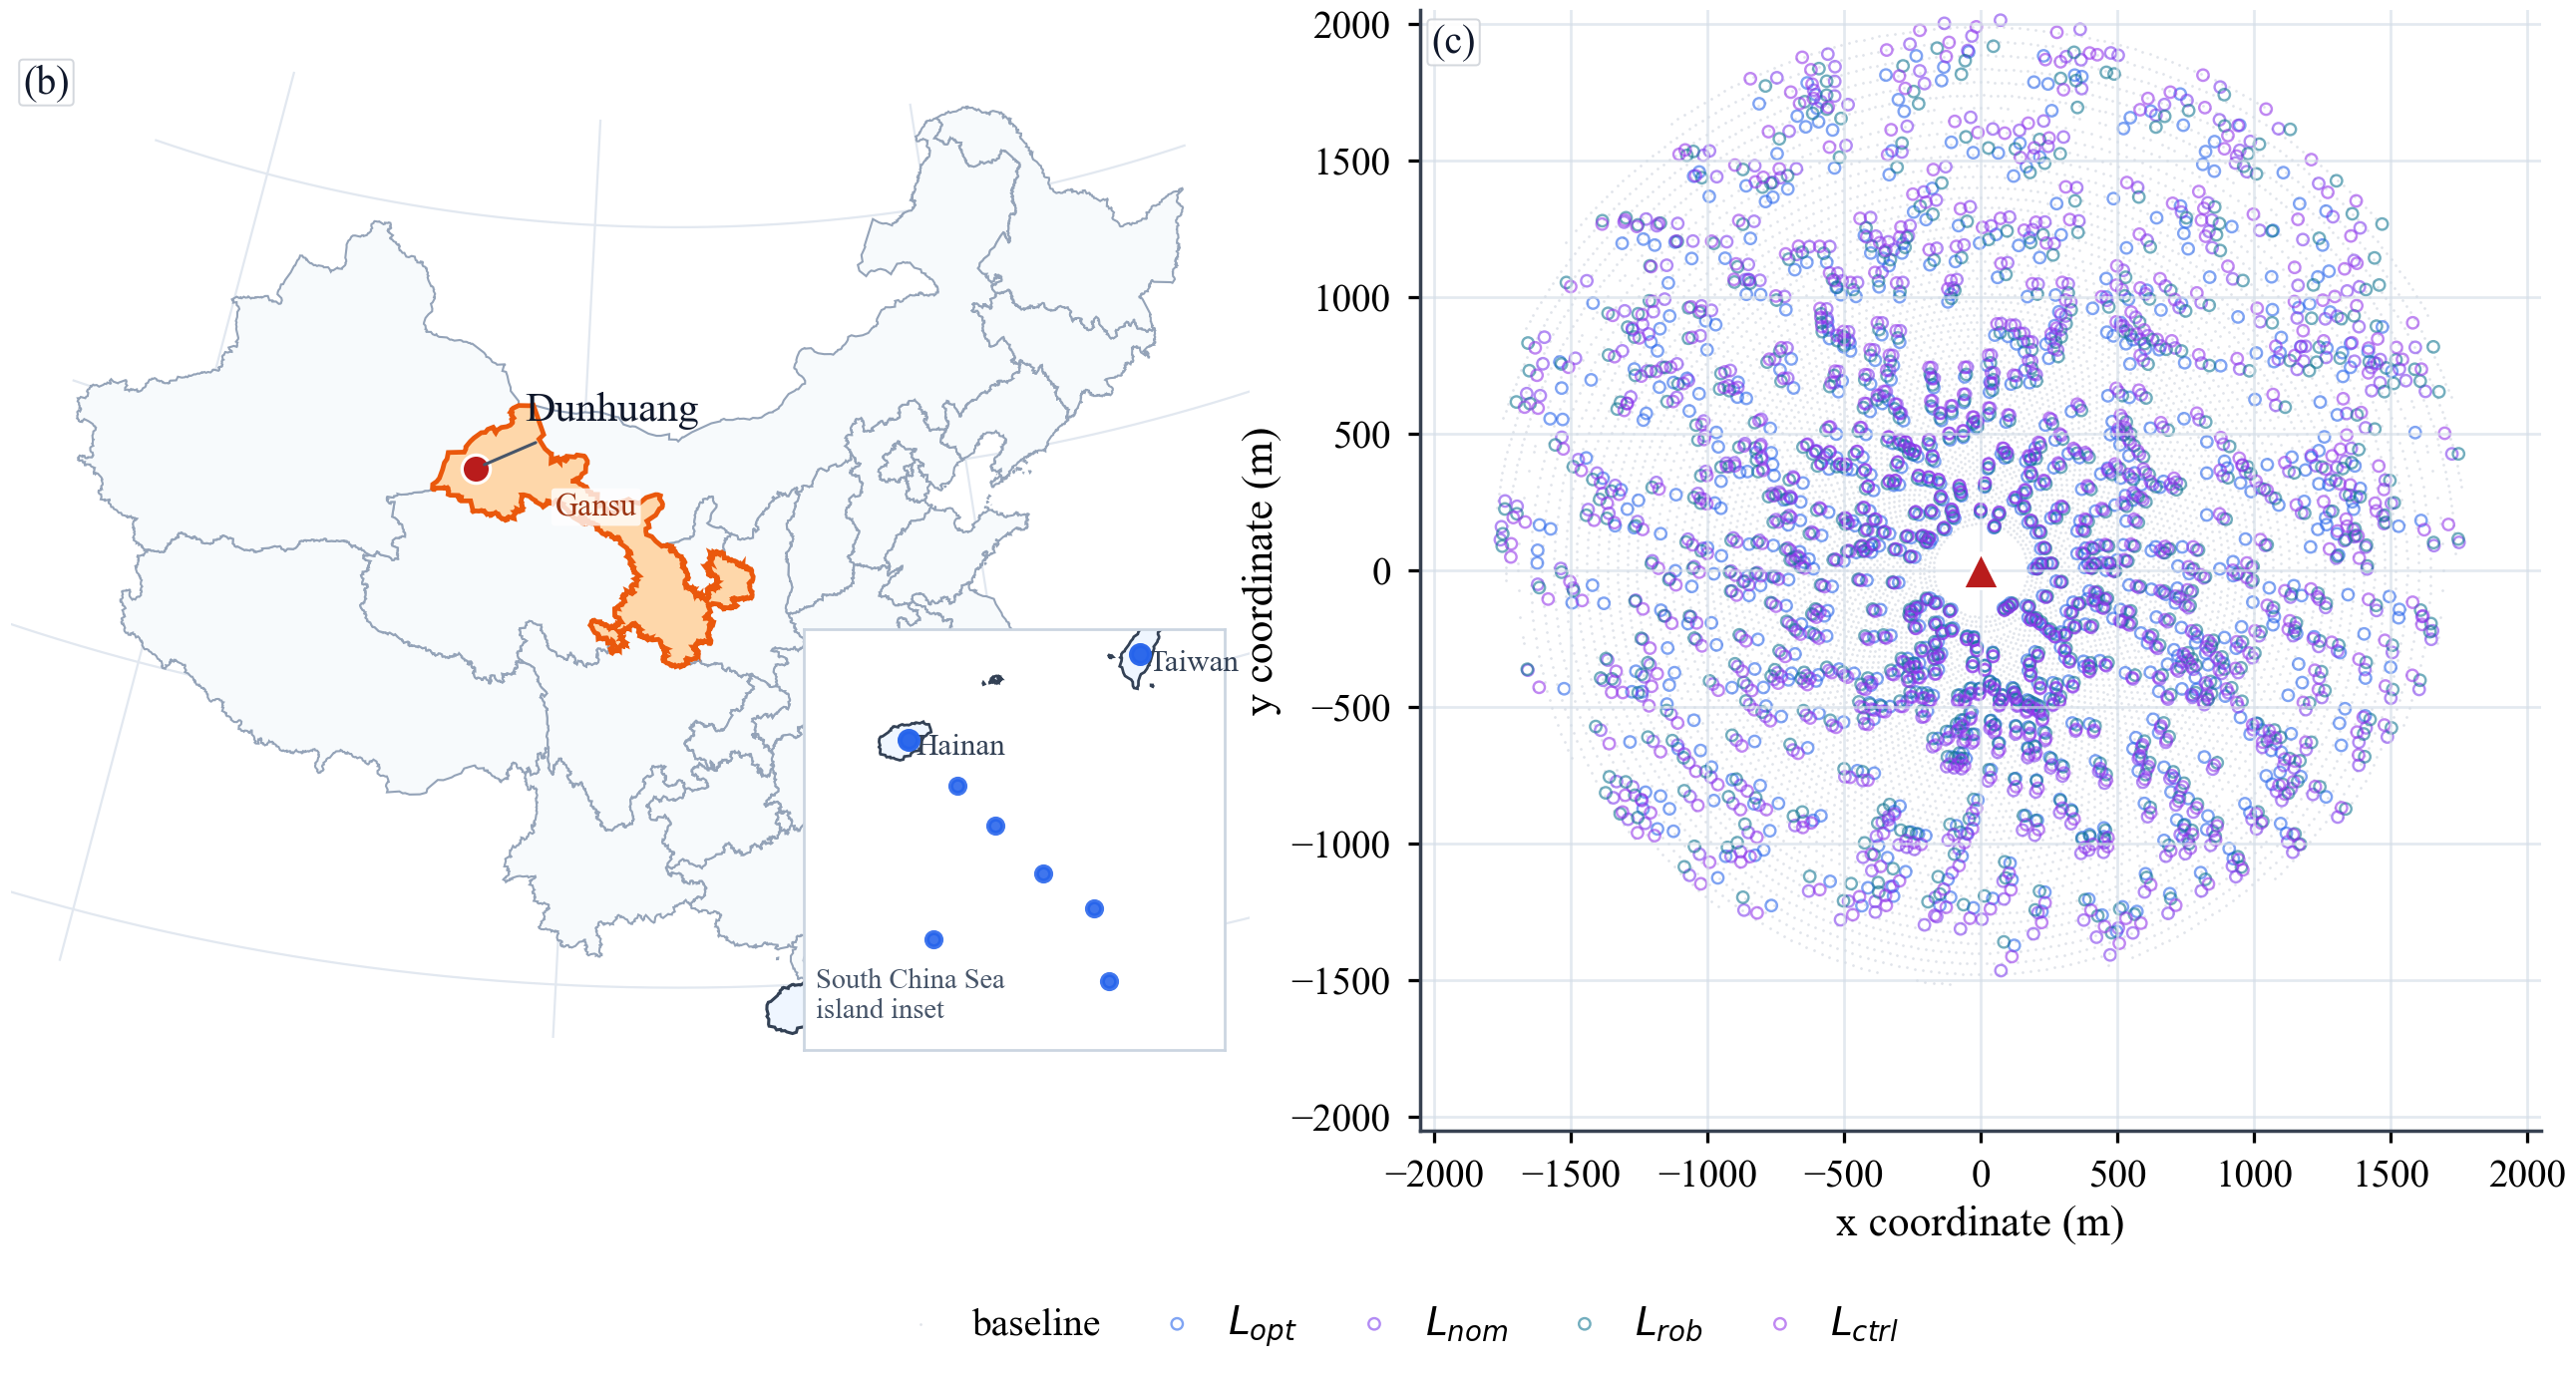
\includegraphics[width=0.94\textwidth]{figures/fig1_locator_geometry_audit.png}
\caption{Field context and full-field geometry audit. Panel (a) is a real Dunhuang heliostat-field aerial photograph taken by co-author Zengye Su using a DJI Mavic 3 Pro drone and is used as qualitative site context only. Panel (b) gives a China-wide projected locator with Gansu highlighted, the Dunhuang site marked, and the Taiwan, Hainan, Hong Kong/Macau-region, and South China Sea island context retained for map completeness. Panel (c) overlays the available 11,915-coordinate heliostat pool and diagnostic samples from representative full-field candidates.}
\label{fig:layout-realism}
\end{figure}
\FloatBarrier

\section{Related Work and Research Gap}
\subsection{Solar tower field modeling and verification tools}
Solar tower modeling tools have evolved from zonal analytical methods toward individual-heliostat and ray-tracing workflows. SolarPILOT applies a Hermite image approach at the individual heliostat level and is integrated with SAM \cite{wagner2018solarpilot,nrel2025pysam}. CoPylot extends the workflow by enabling Python-based interaction with SolarPILOT and custom aimpoint use cases \cite{hamilton2022copilot}. Sunshape and slope-error verification studies show why tool-level optical assumptions matter \cite{wang2020sunshape}. The recent SolTrace--Solstice--TieSOL round-robin study further shows that commercial-scale receiver-flux verification depends on heliostat geometry, focus, canting, and aimpoints, not merely on field coordinates \cite{mitchell2025roundrobin}.

\subsection{Aiming strategy and receiver-flux control}
Receiver aiming has a long line of work. Early optimized aiming for THEMIS, uniform flux strategies, multi-objective cavity-receiver aiming, multi-focal cavity receivers, external receiver aiming, and ant-colony aimpoint optimization established that flux distribution and spillage must be optimized together \cite{salome2013themis,besarati2014uniform,wang2017nsga,yu2014multifocal,astolfi2017external,belhomme2014ant}. Molten-salt receiver work introduced allowable flux-density constraints and translated thermal safety into aiming input \cite{sanchez2017towards,sanchez2017allowable,sanchez2020allowable}. A recent review of heliostat aiming strategies confirms that the field is now judged by the joint treatment of optical gain, receiver uniformity, dynamic operation, and verification realism rather than by one static flux map \cite{li2026aimingreview}. More recent work uses GPU acceleration, flux feedback, closed-loop management, dynamic aiming, model-predictive control under clouds, machine-learning MPC, and real-time swarm methods \cite{oberkirsch2021gpu,acosta2021fluxfeedback,oberkirsch2023closedloop,richter2021dynamic,zhu2023mpc,wu2026mlmpc,zhu2024swarm}.

\subsection{Learning, differentiable optics, and data-driven receiver models}
Learning-based and differentiable methods are now changing the expectations for heliostat aiming papers. Reinforcement-learning aiming has been studied both as real-time strategy optimization and as performance-improving operational control \cite{cruz2022rl,carballo2025rl}. Neural surrogates learn heliostat-to-receiver flux interactions and support tractable optimization \cite{alcantara2025nn}. Differentiable rasterization, differentiable ray tracing for canting, and differentiable Monte Carlo ray tracing turn flux formation into a gradient-aware optimization problem \cite{zheng2025diffneg,grange2025canting,lin2025dmcrt}. Data-driven receiver-level flux prediction further suggests that operational calibration data may complement physics-based ray tracing \cite{schiricke2025fluxprediction}. These methods need realistic full-field test cases; they are not well served by small synthetic fields or mirror-deletion layouts.

\subsection{Layout generation and terrain-screened field design}
Classical field layout studies include preliminary surround-field design, regular field generation, thermochemical-field optimization, quick design of commercial regular fields, load-following layout optimization, no-blocking layouts, multi-objective plant enhancement, robust solar tower optimization under uncertainty, and heliostat-shape-aware field design \cite{collado2009surrounding,collado2012campo,noone2011thermochemical,noone2019quick,ghirardi2021loadfollowing,derbal2023noblocking,guo2020multiobjective,li2022robust,chen2020shapes}. Recent studies add optical-thermal-mechanical coupling, deformable petal hybrid layouts, uneven-terrain layout tooling, sloped-terrain spatiotemporal optimization, collision-analysis-based field design, fast preliminary design tools, and fast annual-energy estimation through heliostat grouping and solar-position sampling \cite{yang2024otm,tang2025petal,ghazanfari2025hefaal,yu2026slopedterrain,adam2026heliosliders,biencinto2025hefesto,liu2026fastannual}. This literature justifies sector/petal deformation as a search family, but it also makes it difficult to claim novelty from petal deformation alone. The research gap for the present manuscript is therefore more specific: a plant-anchored, full-field, terrain-audited, receiver-flux-aware candidate-generation benchmark for a public 100 MW surround field.

The same literature also motivated an explicit strong-baseline pressure test in the revised experiment. The pressure test does not claim to reproduce HelioSliders, HeFAAL, modified artificial-bee-colony, or other named optimizers; doing so would require their full original objective functions, constraints, and implementation details. Instead, it constructs four same-anchor approximation families that capture the type of design freedom emphasized by recent work: low-frequency pattern-free sector/ring deformations, slider-like ringwise azimuthal shifts, terrain-relief-aware redistribution, and hybrid petal/slider pressure layouts. All candidates preserve the 11,915 heliostats and pass through the same SolarPILOT default-aiming and aiming-proxy pipeline. This makes the comparison useful as a pressure test while keeping the method claim conservative.

\subsection{Plant realism, heliostat technology, and benchmark need}
The broader CSP context also matters. Heliostat development roadmaps and HelioCon reports emphasize cost reduction, optical quality, calibration, and field performance as system-level challenges \cite{pfahl2017progress,zhu2022roadmap,zhu2023heliocon,zhu2024helioconannual}. Gen3 CSP and solar-fuel work indicate that receiver thermal input and flux control remain central to high-temperature solar tower applications \cite{turchi2021gen3,zoller2022solarfuels}. New heliostat concepts and wind-induced slope-error studies remind us that layout interacts with structural and terrain effects \cite{freeman2025tiltroll,li2026windslope}. The Dunhuang plant report provides the public anchor for this benchmark \cite{huang2024dunhuang}, while NASA POWER and SRTM provide reproducible but imperfect public weather and terrain layers \cite{nasa2023power,usgs2015srtm}.

\begin{table}[t]
\centering
\caption{Literature map used to position the manuscript.}
\label{tab:lit-map}
\small
\begin{tabular}{p{0.28\textwidth}p{0.62\textwidth}}
\toprule
Theme & Representative references \\
\midrule
Solar tower tools and verification & \cite{wagner2018solarpilot,hamilton2022copilot,mitchell2025roundrobin,wang2020sunshape,nrel2025solarpilotdocs,nrel2025pysam} \\
Receiver aiming and flux control & \cite{li2026aimingreview,salome2013themis,besarati2014uniform,wang2017nsga,yu2014multifocal,astolfi2017external,belhomme2014ant,sanchez2017towards,sanchez2017allowable,sanchez2020allowable} \\
Online, robust, and data-driven aiming & \cite{acosta2021fluxfeedback,oberkirsch2021gpu,oberkirsch2023closedloop,cruz2022rl,richter2021dynamic,zhu2023mpc,wu2026mlmpc,zhu2024swarm,kuhnke2020robust,sanchez2024experimental,carballo2025rl,lin2025dmcrt,zheng2025diffneg,alcantara2025nn,schiricke2025fluxprediction,grange2025canting} \\
Field layout and candidate generation & \cite{collado2009surrounding,collado2012campo,noone2011thermochemical,noone2019quick,ghirardi2021loadfollowing,derbal2023noblocking,guo2020multiobjective,li2022robust,chen2020shapes,tang2025petal,biencinto2025hefesto,ghazanfari2025hefaal,yu2026slopedterrain,adam2026heliosliders,yang2024otm,liu2026fastannual} \\
Plant realism and technology context & \cite{huang2024dunhuang,pfahl2017progress,zhu2022roadmap,zhu2023heliocon,zhu2024helioconannual,zoller2022solarfuels,turchi2021gen3,nasa2023power,usgs2015srtm,freeman2025tiltroll,li2026windslope} \\
\bottomrule
\end{tabular}
\end{table}

\section{Problem Definition}
The design task is to generate full-field Dunhuang-scale candidate layouts that remain physically plausible while revealing whether small geometric changes can improve optical performance without worsening receiver-flux concentration. Let the baseline coordinate set be $\mathcal{H} = \{(x_i,y_i,z_i)\}_{i=1}^N$ with $N=11915$. The coordinate pool is derived from the MIT-licensed author-curated Dunhuang benchmark archive \cite{zaihu2025dunhuangdataset}, specifically the baseline \path{layout_A.csv} file, after removing an origin placeholder and retaining all non-origin coordinate records. It is not claimed to be the official as-built survey of the operating plant. The public plant report gives $11935$ heliostats \cite{huang2024dunhuang}; the missing 20 coordinates are disclosed, not synthetically completed. The missing fraction is 0.17\%, and all candidate comparisons, imported coordinate files, and percentage changes are therefore normalized to the same available $N=11915$ pool. A random-omission geometry audit, reported in the supplementary package, removes 20 heliostats from the available field over 2000 seeded replicates; the 95th-percentile absolute change in mean field radius is 0.33 m and sector/annular coverage remains complete. This supports the stability of the available coordinate pool for geometry benchmarking, while preserving the boundary that the unavailable records are not reconstructed. SRTM90m terrain is then interpolated to the coordinates and stored as tower-relative $z_m$ for public-terrain screening. Each candidate is a transformation $T_\theta(\mathcal{H})$ parameterized by a vector $\theta$ containing bounded radial, azimuthal, scale, twist, and petal terms.

The algorithm has three design constraints. Field-completeness requires $|T_\theta(\mathcal{H})|=N$. Geometry realism requires complete sector and annular coverage, stable nearest-neighbor spacing, bounded axis ratio, and a field envelope visually consistent with the reference surround field. Public-terrain screening requires that the transformed field remain within conservative SRTM90m elevation-range and p95-slope bounds. Receiver safety requires that candidate ranking consider a receiver-flux-risk metric rather than optical efficiency alone.

The objective is a candidate-queue problem rather than a single scalar optimum:
\begin{equation}
\Theta_F=\{\theta\in\Theta:\;T_\theta(\mathcal{H})\ \mathrm{passes\ count,\ geometry,\ spacing,\ extent,\ and\ terrain\ gates}\},
\end{equation}
\begin{equation}
Q=\operatorname{queue}\left(\Theta_F;\; f_1(\theta), f_2(\theta), f_3(\theta)\right),
\quad
f_1=\Delta \eta_{opt},\quad
f_2=-\Delta R_{flux},\quad
f_3=-\Delta R_{aim}.
\end{equation}
Here $\Delta \eta_{opt}$ is the SolarPILOT mean optical-efficiency change, $\Delta R_{flux}$ is the default-aiming peak-to-active-mean receiver-flux change, and $\Delta R_{aim}$ is the screening-level proxy peak-to-mean change under searched staggered aiming. The queue operator denotes representative selection over candidate roles rather than a unique Pareto optimum. Each reported role is tied to the evidence layer that supports it: proxy-only, SolarPILOT default-aiming numerical verification, or reduced PySolTrace direct-aimpoint check.

\begin{table}[t]
\centering
\caption{How the revised problem definition differs from a descriptor-only layout comparison.}
\label{tab:reframe}
\small
\begin{tabular}{p{0.25\textwidth}p{0.29\textwidth}p{0.34\textwidth}}
\toprule
Dimension & Descriptor-only comparison & Revised benchmark logic \\
\midrule
Primary object & Two exported layouts & A plant-scale candidate-generation and verification pipeline \\
Field scale & One baseline and one mirror-reduced case & All representatives preserve the available 11,915-coordinate field \\
Novelty claim & Dataset reuse value & Public plant anchor, receiver-flux evidence ladder, and reproducible candidate queue \\
Physical realism & Weak because mirror deletion changes plant scale & Stronger because count, envelope, coverage, terrain, and receiver metrics are audited \\
Verification & Annual SAM comparison only & PySAM/SolarPILOT layout verification plus custom-aimpoint queue \\
Claim risk & Looks like default software output & Becomes an auditable, bounded engineering method with clear next-stage verification \\
\bottomrule
\end{tabular}
\end{table}

The formulation treats layout and aiming as coupled plant-scale decisions. A layout that slightly improves cosine efficiency may concentrate more heliostats onto a receiver zone under default aiming, while a layout that looks safer in receiver flux may lose field efficiency. The practical output is therefore a queue of candidates and evidence about why each candidate is interesting, not a single coordinate file declared optimal.

\section{Terrain-Screened Full-Field Candidate Generation}
\subsection{Inputs and constraints}
The TS-FPDA input consists of the baseline coordinates, audited plant parameters, a public terrain grid, a weather file, and bounds on deformation parameters. In this paper TS-FPDA is used as a conservative candidate-generation workflow, not as a claim of global field optimality. The field transformation preserves heliostat identity and count. This is essential because mirror deletion changes the plant scale and confounds optical, economic, and receiver comparisons.

\subsection{Coordinate transformation family}
The candidate transformation combines bounded global scaling, radial scaling, radial wave perturbation, angular twist, azimuthal wave perturbation, north-south bias, and petal deformation. A candidate point $(x_i,y_i)$ is first converted to tower-centred polar coordinates $(r_i,\phi_i)$, with $\rho_i=r_i/r_{\max}$. The implementation uses $\phi_i=\arctan2(x_i,y_i)$ so that north-south bias is applied consistently with the plant coordinate convention. For a petal order $k_p>0$, define $p_i=\cos[k_p(\phi_i-\psi_p)]$; otherwise $p_i=0$. The transformed point is:
\begin{align}
r_i' &= r_i\{1+s_r+a_r\cos(2\phi_i)\rho_i+a_p p_i\rho_i^{1.4}+b_n\cos(\phi_i)\rho_i\},\\
\phi_i' &= \phi_i+\omega \rho_i^{1.25}+a_\phi\sin(2\phi_i)\rho_i+\omega_p\sin[k_p(\phi_i-\psi_p)]\rho_i^{1.15},\\
x_i' &= s_x r_i' \sin(\phi_i'),\\
y_i' &= s_y r_i' \cos(\phi_i').
\end{align}
The coefficient bounds are listed in Table~\ref{tab:param-envelope}. Petal deformation is therefore introduced through low-order sector modulation rather than arbitrary random displacement. The deformation family is intentionally conservative; novelty comes from the full-field verification workflow, not from extreme geometry.

\subsection{Algorithm listing}
Table~\ref{alg:tfpda} gives the reproducible version of the workflow. The implementation uses the same logic but stores intermediate tables so that every exported layout can be traced back to its parameter vector, proxy metrics, verification settings, and checksum. This audit trail is essential because modest layout improvements are credible only when the method is transparent enough to reproduce.

\begin{longtable}{p{0.08\textwidth}p{0.82\textwidth}}
\caption{TS-FPDA: terrain-screened full-field candidate-generation workflow.}
\label{alg:tfpda}\\
\toprule
Step & Operation \\
\midrule
1 & Load the raw layout file, remove tower-origin placeholders, and define the invariant coordinate set $\mathcal{H}$ with $N=11915$. \\
2 & Interpolate public SRTM90m elevation to each heliostat location and convert absolute elevation to tower-relative terrain height $z_m$. \\
3 & Sample a bounded deformation vector $\theta=(s_x,s_y,s_r,a_r,\omega,a_\phi,a_p,k_p,\psi_p,\omega_p,b_n)$. \\
4 & Transform every heliostat using the radial, azimuthal, twist, and petal equations while preserving heliostat identity and count. \\
5 & Run hard feasibility gates: heliostat count, finite coordinates, sector coverage, annular coverage, field extent, axis ratio, spacing, terrain range, and p95 slope. \\
6 & Compute proxy optical contribution, cost-normalized screening score, flux-risk index, and layout-quality score for every feasible candidate. \\
7 & Select representatives by role: baseline control, maximum proxy energy, cost-normalized screening case, minimum proxy flux risk, balanced, and extra balanced candidates. \\
8 & Export layout CSV files, candidate tables, figures, and manifest hashes before higher-fidelity numerical checking. \\
9 & Import selected layouts into PySAM/SolarPILOT using the same plant parameters and default-aiming settings. \\
10 & Report optical-efficiency and receiver-flux changes, then use the aiming proxy and reduced SolTrace tests to prioritize full-field or annual custom-aimpoint verification. \\
\bottomrule
\end{longtable}

\subsection{Parameter envelope}
Table~\ref{tab:param-envelope} summarizes the parameter envelope. These are not universal design limits; they are local-search limits chosen to keep the generated candidates near the audited Dunhuang field. A larger search envelope could find stronger apparent gains, but it would also increase the risk of creating a field that no longer resembles the public plant.

\begin{table}[t]
\centering
\caption{Deformation parameters and their manuscript role. Numeric values are interpreted as conservative local-search amplitudes around the audited field.}
\label{tab:param-envelope}
\small
\begin{tabular}{p{0.23\textwidth}p{0.29\textwidth}p{0.36\textwidth}}
\toprule
Parameter family & Typical range or role & Rationale \\
\midrule
Global x/y scale, $s_x,s_y$ & Deterministic grid: 0.97, 0.99, 1.01, 1.03; random range: 0.965--1.035 & Allows mild anisotropic expansion or compression while keeping the field elliptical. \\
Radial redistribution, $s_r,a_r$ & $s_r=-0.025$--0.025; $a_r=-0.018$--0.018 with $\cos(2\phi)\rho$ & Allows inward/outward and sector-dependent ring changes without changing heliostat count. \\
Azimuthal deformation, $\omega,a_\phi$ & $\omega=-0.035$--0.035 rad; $a_\phi=-0.020$--0.020 rad & Represents smooth twist and stagger-like movement rather than random point displacement. \\
Petal family, $a_p,k_p,\psi_p,\omega_p$ & $k_p\in\{0,4,6,8\}$; $a_p=-0.026$--0.026; bounded phase and petal-twist terms & Connects to recent petal and hybrid layout ideas while avoiding decorative overfitting. \\
North bias, $b_n$ & Random range: -0.012--0.012 multiplied by $\cos(\phi)\rho$ & Allows the northern-hemisphere cosine-bias effect to appear without converting the field into a north-only design. \\
Terrain assignment & SRTM-derived tower-relative elevation & Adds reproducible terrain screening while remaining honest about resolution limits. \\
\bottomrule
\end{tabular}
\end{table}
\FloatBarrier

\subsection{Feasibility filters}
Each candidate is filtered by count, coverage, spacing, axis ratio, terrain range, terrain slope, and publishable-geometry flags. The sector coverage and annular coverage constraints prevent field collapse. The nearest-neighbor constraint discourages unrealistic local crowding. The axis-ratio constraint keeps the field envelope elliptical rather than fragmented.

\begin{table}[t]
\centering
\caption{Candidate-screening gates used to keep the field complete and engineering-plausible.}
\label{tab:gates}
\small
\begin{tabular}{p{0.22\textwidth}p{0.28\textwidth}p{0.38\textwidth}}
\toprule
Gate & Failure mode caught & Engineering rationale \\
\midrule
Count preservation & Deleted or duplicated heliostats & Prevents the study from changing commercial plant scale. \\
Origin filtering & Tower placeholder treated as heliostat & Protects spacing and extent statistics. \\
Sector coverage & Missing azimuthal sectors & Prevents collapse into a partial field. \\
Annular coverage & Missing radial bands & Keeps inner, middle, and outer field structure. \\
Nearest-neighbor spacing & Local crowding after deformation & Approximates access and collision realism before detailed road modeling. \\
Extent and axis ratio & Unphysical elongation or fragmentation & Keeps the field near a surround/ellipse envelope. \\
Terrain range and p95 slope & Movement into terrain outliers & Ensures screened candidates remain close to the public site slope. \\
SolarPILOT importability & Coordinates rejected or simulation instability & Ensures selected representatives can be independently checked. \\
\bottomrule
\end{tabular}
\end{table}

The gates also provide an engineering interpretation of the visual layout preview. A complete annular or ellipse-like field is not suspicious for this plant; it is the expected outcome after the candidate-generation gates forbid mirror deletion and sector loss. What would be suspicious is a candidate with large holes, radial collapse, disconnected islands, or an unexplained reduction in heliostat count. The current candidates are kept conservative so that the search stays inside a credible local design neighbourhood.

\subsection{Benchmark settings and traceability}
Earlier versions of the workflow left too many numerical defaults embedded only in scripts. For the journal manuscript, the detailed parameter registry is moved to the reproducibility package, and the main text keeps only the settings needed to interpret the results. The benchmark uses the public Dunhuang location at 40.063$^\circ$N, 94.426$^\circ$E, a NASA POWER-derived SAM weather file, the audited 11,915-coordinate pool, the public tower/receiver/heliostat dimensions in Table~\ref{tab:plant-audit}, 1,841 screened full-field candidates, geometry gates over 36 sectors and 12 annuli, a 48-sector by 8-annulus aiming proxy, common PySAM/SolarPILOT default-aiming checks with 24 by 24 receiver maps and eight flux days, and reduced PySolTrace audits over 27 paired solar conditions. These settings are fixed in \path{reproducibility_config/}, \path{code/configs/server_full.json}, and the checksum manifest, so the paper can describe the workflow without reproducing a directory listing.

\subsection{Proxy screening}
Proxy annual optical contribution, a cost-normalized screening score, and flux-risk metrics are used only for candidate triage. The optical proxy estimates relative field contribution under a simplified solar-position and loss model. The cost-normalized score is not an LCOE model: it does not include tower redesign, receiver redesign, O\&M, storage dispatch, financing, or discounted annual energy. It is retained only to keep the representative queue from ignoring plant-scale cost intuition while all candidate layouts preserve the same heliostat count. The flux-risk proxy identifies angular concentration patterns that may become receiver hot spots under aiming.

For a candidate $\theta$, the screening layer uses normalized terms
\begin{equation}
S_E(\theta)=E_{proxy}(\theta)/E_{proxy}(0),\quad
S_C(\theta)=C_{proxy}(\theta)/C_{proxy}(0),\quad
S_F(\theta)=R_{proxy}(\theta)/R_{proxy}(0),
\end{equation}
where $E_{proxy}$ is the simplified optical-contribution proxy, $C_{proxy}$ is the cost-normalized screening score, and $R_{proxy}$ is the receiver peak-to-active-mean proxy. The score $S_C$ is not an economic-superiority metric; it is used only to choose a diverse representative queue for later numerical checking.

\subsection{Representative selection}
Representatives are selected to cover the candidate frontier: baseline, maximum proxy energy, cost-normalized screening case, minimum proxy flux risk, balanced layouts, and additional balanced candidates. This selection prevents the paper from depending on one cherry-picked result. It also creates controls for reduced and enlarged custom-aimpoint checks.

\subsection{Implementation traceability}
The implementation is written so that tables, figures, and quantitative claims are generated from the same audited run directory. Candidate generation, proxy screening, SolarPILOT numerical checking, reduced PySolTrace direct checks, figure generation, and checksum construction are all represented by separate scripts in the released package. The main text does not reproduce a file-by-file script inventory; instead, the package manifest links each claim family to its source tables and checksums. This structure reduces the risk that manuscript text, figures, and verification tables drift apart during revision.

The runtime design separates fast screening from slower verification. The deformation layer can screen hundreds of conservative candidates, while SolarPILOT is reserved for representative layouts. This division is a practical compromise: the proxy cannot establish final optimality, but ray-tracing every small local deformation is also inefficient. The result is a reproducible screening-to-checking funnel, a common pattern in engineering optimization studies.

Viewed as a benchmark system, the workflow has a deliberate closed loop. Candidate generation proposes bounded full-field perturbations; feasibility gates reject geometrically or terrain-wise implausible variants; proxy metrics choose a small and diverse screening queue; SolarPILOT exposes whether optical gains create default receiver-flux penalties; and reduced direct ray tracing tests whether aimpoint redistribution can change the receiver-risk ranking. When a verification layer contradicts an earlier proxy, the mismatch is used to refine the evidence boundary and the next screening queue. This is the main reason the paper is framed as a benchmark and workflow contribution rather than as a one-shot optimization study. The retained audit groups are the coordinate audit, candidate-generation tables, aiming-proxy screen, SolarPILOT default-aiming outputs, reduced direct checks, figure-generation scripts, and checksum manifests; file-level names and SHA-256 hashes are provided in the supplementary manifest.

\subsection{Computational workload and audit scale}
The workload tied to the current claims is reported as audit context rather than as a cross-machine performance benchmark. The screened full-field search produced 1,841 conservative candidates, the joint layout--aiming layer evaluated 489 publishable candidates with 23 aiming strategies per candidate, the high-resolution SolarPILOT bridge checked five representative layouts with 86 receiver-flux maps per layout, and the first all-phase reduced PySolTrace matrix traced 1,485 layout--strategy--condition cases. In that all-phase matrix, the recorded runtime averaged 6.24 s per case, with a maximum of 11.05 s and a total recorded case runtime of 154.46 min. Later baseline-control, hold-out, joint-promotion, high-sample, independent-seed, and 240k-ray follow-up audits enlarge the evidence base, but their detailed row counts and runtime tables are kept in the supplementary package. This presentation keeps the article focused on the scientific evidence while preserving reproducibility for reviewers.

\section{Receiver-Aiming Proxy}
The proxy divides heliostats into azimuthal sectors and radial annuli. Each group contributes a Gaussian-like spot on an unwrapped cylindrical receiver map. The contribution is weighted by optical contribution and adjusted by the selected aimpoint rule. Three strategy families are evaluated: equator aiming, five-point aiming, and nine-level staggered aiming. The metrics are intercept fraction, spillage proxy, peak-to-active-mean concentration, and active-zone coefficient of variation.

The proxy has two purposes. First, it checks whether layout changes alter the receiver distribution in a way that default SolarPILOT aiming cannot reveal. Second, it identifies the most informative layouts for direct custom-aimpoint testing. It is not used as a final claim. For a high-fidelity layout--aiming co-design claim, the proxy must be followed by direct ray-tracing or SolarPILOT/CoPylot verification.

\subsection{Proxy metrics}
The receiver proxy reports four metrics. The intercept proxy estimates the fraction of reflected power falling inside the active receiver map. The spillage proxy records the complementary lost fraction. The peak-to-active-mean ratio measures concentration relative to the illuminated receiver zone, which is more informative than comparing a peak value with the mean of an entire map containing inactive cells. The active-zone coefficient of variation measures distribution uniformity. A candidate is considered interesting only if it improves at least one receiver-risk metric without destroying intercept.

\begin{table}[t]
\centering
\caption{Receiver-aiming proxy metrics and how they are used.}
\label{tab:proxy-metrics}
\small
\begin{tabular}{p{0.25\textwidth}p{0.29\textwidth}p{0.34\textwidth}}
\toprule
Metric & Interpretation & Manuscript use \\
\midrule
Intercept fraction proxy & Fraction of proxy energy on the active receiver map & Rejects aiming strategies that reduce peak flux by simply spilling energy. \\
Spillage proxy & Proxy energy outside receiver bounds & Flags unsafe or inefficient aiming distributions. \\
Peak-to-active-mean ratio & Maximum flux divided by active-zone mean & Primary hot-spot risk metric for candidate queueing. \\
Active-zone coefficient of variation & Spatial uniformity of illuminated map & Secondary receiver-uniformity metric. \\
Best strategy label & Strategy family, spread, and phase identifier & Makes the custom-aimpoint candidate reproducible. \\
\bottomrule
\end{tabular}
\end{table}

The proxy is intentionally positioned below the SolarPILOT numerical-checking layer. It is useful because it can scan aiming families quickly, but it omits detailed heliostat images, canting, sunshape, slope error, and receiver geometry handled by higher-fidelity tools. The paper therefore uses proxy results as a triage system. The manuscript separates claims checked by SolarPILOT from claims promoted to reduced direct ray tracing, and keeps both below full-field annual certification.

\section{Joint Layout--Aiming Screening Layer}
The strict-review strengthening exposed a limitation in the first workflow: layout generation and aiming selection were mostly sequential. The deformation algorithm generated full-field candidates, and the aiming proxy then searched strategies for a small representative queue. That structure is useful for auditing, but it is not yet a complete layout--aiming optimization system. A joint screening layer was therefore added after the baseline-control audits. It preserves the same 11,915-heliostat coordinate pool and the same geometry gates, but evaluates layout deformation parameters and receiver-aiming strategies inside one loop.

For each candidate $\theta$, the joint layer computes the same geometry, terrain, and optical-proxy descriptors as TS-FPDA, then searches a fixed aiming set $\mathcal{A}$ containing visible-equator, five-point, S9 staggered phases, and balanced spread strategies. The best strategy is selected by the screening objective
\begin{equation}
a^*(\theta)=\arg\min_{a\in\mathcal{A}}\left[
R_{aim}(\theta,a)+0.75\,CV_{active}(\theta,a)+7.0\,S_{spill}(\theta,a)
\right],
\end{equation}
where $R_{aim}$ is the proxy peak-to-active-mean receiver ratio, $CV_{active}$ is the active-zone coefficient of variation, and $S_{spill}$ is the proxy spillage fraction. Candidate ranking then uses a scalarized loss
\begin{equation}
\mathcal{L}_{joint}(\theta)=100\left(\frac{R_{aim}(\theta,a^*)}{R_{aim}(0,a_0^*)}-1\right)
-55\left(\frac{E_{proxy}(\theta)}{E_{proxy}(0)}-1\right)
\Pi_{spill}+\Pi_{geom},
\end{equation}
where $\Pi_{spill}$ and $\Pi_{geom}$ penalize extra spillage, reduced layout quality, crowding, and terrain outliers. The coefficients intentionally favour receiver-risk reduction only when geometry remains publishable and optical loss is small. They are not universal design weights; they define a reproducible screening queue for this Dunhuang benchmark.

The search is seeded from the earlier full-field candidate table and from additional bounded random deformations, followed by elite mutation over four generations. The manuscript-facing run evaluates 489 candidates, tests 23 aiming strategies for each candidate, and exports all candidate rows, Pareto rows, representative layouts, convergence plots, and layout overlays. This joint layer is still below direct ray tracing in the evidence ladder. Its purpose is to produce more coherent layout--aiming hypotheses for SolarPILOT, CoPylot, SolTrace, or Solstice checks, not to certify annual plant operation.

\section{PySAM/SolarPILOT Numerical Verification}
Representative layouts are imported into PySAM/SolarPILOT through \path{helio_positions_in}. The numerical check uses audited heliostat, tower, receiver, and cost parameters and a SAM-compatible NASA POWER weather file. The high-resolution run evaluates five layouts in total---the baseline plus four representative deformations---with \path{flux-days = 8}, \path{flux-bins = 24}, and 86 flux maps per layout. Terrain-relative $z_m$ and custom aimpoint coordinates are not represented in the current PySAM bridge, so this layer is a default-aiming layout-level check.

This protocol is intended for reproducible benchmark development rather than final industrial design certification. Its value comes from making the verification layer explicit: imported layouts are tested under the same SolarPILOT settings, while terrain-relative elevation and custom aimpoints remain outside the current PySAM bridge.

A second, reduced direct-check layer is added for custom aiming. PySolTrace was built from the NREL SolTrace source with the native \path{coretrace_api.so} backend and used to trace stratified samples of the full field. The implementation verifies that the heliostat reflector stage precedes the receiver absorber stage, so rays are reflected by the sampled field before being binned on the receiver. The cylindrical receiver is approximated by flat absorber panels with the public 15.13 m diameter and 18.6 m height. The enlarged all-phase matrix uses 6,000 sampled heliostats per layout, 60,000 requested first-stage ray hits per case, 27 solar conditions, visible-equator aiming, five-point aiming, and all nine S9 staggered phases on an 18-panel receiver approximation. Receiver intercept ratios in this all-phase matrix range from approximately 0.639 to 0.748, providing a simple stage-order sanity check. A separate high-sample confirmation matrix then repeats the same 27 solar conditions for five verification-relevant strategies using 9,000 sampled heliostats, 180,000 requested first-stage ray hits, 24 receiver panels, and a 24 by 72 receiver grid. An independent-seed replicate repeats the high-sample scale with a fresh stratified sample. A final V12 follow-up keeps the same five layouts, five verification-relevant strategies, and 27 solar conditions, but increases the requested first-stage ray hits to 240,000 per case. Across the consolidated reduced direct-check layers, receiver intercept ratios span approximately 0.636--0.748. These layers are reported as reduced direct checks because they use sampled heliostats and representative solar conditions rather than a full-field annual ray-tracing campaign.

A schematic summary of this funnel is shown in Fig.~\ref{fig:workflow}. The diagram separates the input audits, bounded full-field candidate generation, candidate queueing, and three verification layers. This distinction matters because the manuscript's strongest claim is not that one deformation is universally optimal, but that the evidence layers can reorder the candidate queue in a reproducible way.

\begin{figure}[t]
\centering
\resizebox{0.98\textwidth}{!}{%
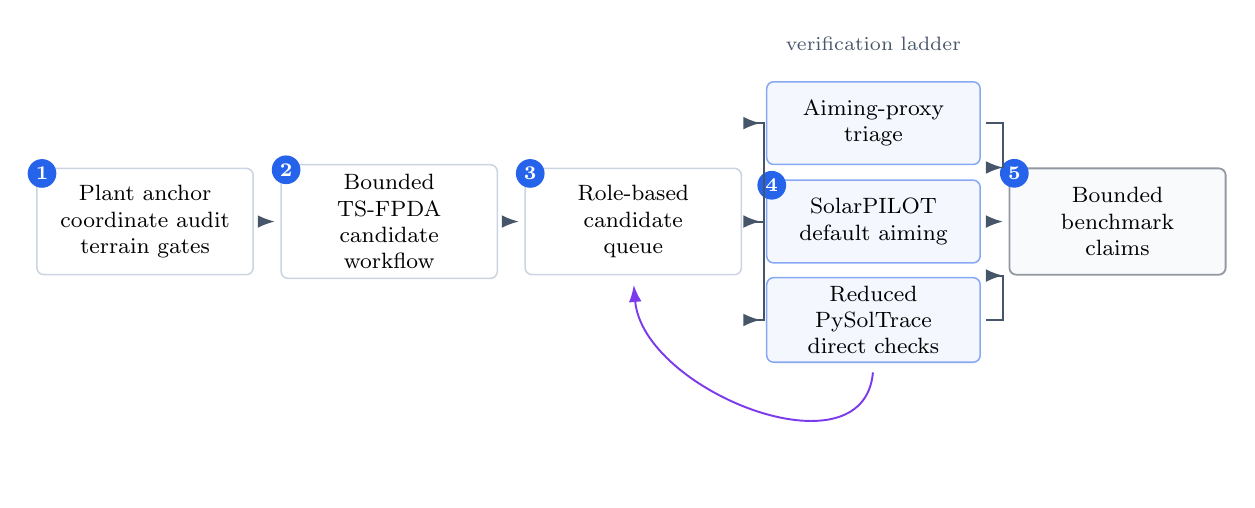
\begin{tikzpicture}[
  font=\rmfamily\footnotesize,
  stage/.style={rectangle,rounded corners=2.5pt,draw=DHFLine,line width=0.55pt,fill=white,text width=25mm,minimum height=13.5mm,align=center,inner sep=3.5pt},
  verify/.style={rectangle,rounded corners=2.5pt,draw=DHFBlue!55,line width=0.55pt,fill=DHFBlue!5,text width=25mm,minimum height=10.5mm,align=center,inner sep=3pt},
  final/.style={rectangle,rounded corners=2.5pt,draw=DHFInk!45,line width=0.65pt,fill=DHFFill,text width=25mm,minimum height=13.5mm,align=center,inner sep=3.5pt},
  dot/.style={circle,draw=none,fill=DHFBlue,text=white,font=\bfseries\scriptsize,inner sep=1.4pt},
  flow/.style={-Latex,line width=0.70pt,draw=DHFMuted,shorten >=2pt,shorten <=2pt},
  feedback/.style={-Latex,line width=0.70pt,draw=DHFPurple,shorten >=2pt,shorten <=2pt}
]
\node[stage] (audit) at (0,0) {Plant anchor\\coordinate audit\\terrain gates};
\node[stage] (gen) at (3.10,0) {Bounded\\TS-FPDA\\candidate workflow};
\node[stage] (queue) at (6.20,0) {Role-based\\candidate\\queue};
\node[verify] (proxy) at (9.25,1.25) {Aiming-proxy\\triage};
\node[verify] (solar) at (9.25,0) {SolarPILOT\\default aiming};
\node[verify] (trace) at (9.25,-1.25) {Reduced\\PySolTrace\\direct checks};
\node[final] (claim) at (12.35,0) {Bounded\\benchmark\\claims};

\foreach \n/\p in {1/audit,2/gen,3/queue,4/solar,5/claim} {
  \node[dot,anchor=north west] at ($(\p.north west)+(-0.06,0.06)$) {\n};
}

\draw[flow] (audit.east) -- (gen.west);
\draw[flow] (gen.east) -- (queue.west);
\draw[flow] (queue.east) -- ++(0.28,0) |- (proxy.west);
\draw[flow] (queue.east) -- (solar.west);
\draw[flow] (queue.east) -- ++(0.28,0) |- (trace.west);
\draw[flow] (proxy.east) -- ++(0.28,0) |- (claim.north west);
\draw[flow] (solar.east) -- (claim.west);
\draw[flow] (trace.east) -- ++(0.28,0) |- (claim.south west);
\draw[feedback] ($(trace.south)+(0,-0.5mm)$) to[out=-95,in=-85,looseness=1.12]
  ($(queue.south)+(0,-0.5mm)$);

\node[font=\scriptsize,text=DHFMuted,anchor=south] at (9.25,2.05) {verification ladder};
\end{tikzpicture}%
}
\caption{Benchmark and numerical-checking workflow as a native TikZ vector schematic. Public plant anchors, coordinate auditing, and terrain/geometry gates feed the bounded TS-FPDA candidate-generation workflow. The candidate queue is then checked through fast aiming-proxy triage, SolarPILOT default-aiming numerical verification, and reduced PySolTrace direct-aimpoint checks before the claim boundary is set. The feedback arrow records that later evidence can reorder the queue, so the output is a reproducible benchmark and screening queue rather than a final commercial redesign.}
\label{fig:workflow}
\end{figure}

\section{Results}
The results are organized as a benchmark-system narrative rather than as a sequence of isolated outputs. The first layer asks whether the workflow can generate plant-scale alternatives without changing the commercial field size or damaging the surround-field envelope. A new same-condition control layer then asks whether the reported behaviour can be explained by simple global transformations alone. The next layer asks whether the apparently better optical candidates remain acceptable when receiver-flux concentration is made visible. The aiming layer uses a fast proxy to form a screening queue, and the reduced direct-ray layer tests where that queue is stable or unstable. This staged interpretation separates controls, screening evidence, numerical checks, and future verification needs.

\subsection{Full-field screening}
The streamed server run evaluated 1,841 conservative full-field candidates and exported eight representatives. All representatives preserve 11,915 heliostats. Terrain elevation ranges remain approximately 33.3--35.2 m for the key high-resolution verification set, and p95 terrain slope remains approximately 1.275--1.280\%. The proxy energy spread is intentionally narrow because no candidate is allowed to delete mirrors or radically distort the field.

The narrow proxy spread is expected for a conservative full-field search. In a mirror-reduced comparison, a field can appear different because the plant scale has changed. In the present run, all candidates stay inside the same full-field design space, so a 1--3\% optical change is interpreted as local-design sensitivity around a real 100 MW surround field. The result is not a global re-optimization of tower height, receiver size, storage, dispatch, roads, or land boundaries.

\begin{table}[t]
\centering
\caption{Representative roles used to prevent cherry-picking.}
\label{tab:representative-roles}
\small
\begin{tabular}{p{0.28\textwidth}p{0.60\textwidth}}
\toprule
Representative role & Selection logic and interpretation \\
\midrule
Baseline control & Audited available full field; establishes the common count, envelope, terrain, and SolarPILOT reference. \\
Maximum proxy energy & Best screening-level optical proxy; tests whether an optical-looking candidate remains useful after numerical checking. \\
Cost-normalized screen & Best cost-normalized screening score; keeps plant-scale cost intuition visible without making an LCOE claim. \\
Minimum flux risk & Lowest screening flux-risk index; tests whether receiver-risk relief comes at an optical-efficiency cost. \\
Balanced & Compromise among energy, cost, flux, and geometry; represents the most publishable candidate class. \\
Balanced extra & Additional non-dominated or near-balanced candidates; checks whether the interpretation depends on one selected point. \\
\bottomrule
\end{tabular}
\end{table}

\subsection{Same-condition baseline controls}
A useful control question is whether the proposed representatives only reproduce simple radial scaling or field stretching. To test that possibility, six low-complexity controls were added and checked under the same public terrain layer, the same 11,915-heliostat coordinate pool, the same PySAM/SolarPILOT default-aiming bridge, and the same aiming-proxy search as the TS-FPDA representatives. The controls are uniform radial compaction, uniform radial expansion, simple anisotropic ellipse scaling, a smooth north/south bias, a two-lobe radial wave, and a pure azimuthal stagger. They are not literature reimplementations and should not be presented as state-of-the-art baselines. Their purpose is narrower: they test whether a simple one- or two-parameter geometric effect is already enough to explain the observed trade-off.

Table~\ref{tab:baseline-controls} and Fig.~\ref{fig:baseline-controls} show that the answer is mixed in a useful way. The simple controls are not trivial. Radial compaction gives a +0.89\% SolarPILOT optical-efficiency gain, but it also raises the default peak-to-active-mean flux ratio by +1.07\%. Radial expansion has the opposite sign, reducing the default flux ratio by -1.04\% but losing -0.89\% optical efficiency. The best simple aiming-proxy control, the two-lobe radial wave, reduces the proxy peak-to-mean ratio by -2.38\% with essentially neutral SolarPILOT optical change. These controls therefore explain part of the field-geometry sensitivity and prevent the manuscript from claiming that every positive signal comes uniquely from TS-FPDA.

At the same time, the controls do not remove the value of the representative queue. The optical-upper TS-FPDA layout $L_{opt}$ still gives the largest SolarPILOT optical gain (+3.15\%), but with the largest default flux-ratio penalty (+4.68\%). The nominal and receiver-risk representatives give larger aiming-proxy reductions than all simple controls: $L_{nom}$ gives -6.22\%, $L_{opt}$ gives -5.48\%, and $L_{rob}$ gives -5.34\%. The correct interpretation is therefore bounded. The workflow is not a globally superior optimizer, but the role-based queue is more informative than a set of simple radial, ellipse, north-bias, wave, and stagger controls under the same numerical assumptions.

\begin{table}[t]
\centering
\caption{Same-condition low-complexity baseline controls and TS-FPDA representatives. All layouts preserve the available 11,915-heliostat coordinate pool. Optical and default-flux changes are from PySAM/SolarPILOT; aiming changes are from the proxy search and remain screening-level evidence.}
\label{tab:baseline-controls}
\scriptsize
\begin{tabular*}{\textwidth}{@{\extracolsep{\fill}}llrrrp{0.28\textwidth}@{}}
\toprule
Layout & Type & $\Delta\eta_{opt}$ (\%) & $\Delta R_{flux}$ (\%) & $\Delta R_{aim}$ (\%) & Interpretation \\
\midrule
$C_{\mathrm{rad}-}$ & radial compact & +0.89 & +1.07 & -0.11 & Optical gain from simple compaction, but default flux worsens. \\
$C_{\mathrm{rad}+}$ & radial expand & -0.89 & -1.04 & +0.10 & Flux relief from simple expansion, but optical efficiency falls. \\
$C_{\mathrm{ell}}$ & ellipse scale & +0.02 & +0.48 & +2.31 & Simple anisotropic scaling is not a receiver-risk improvement. \\
$C_{\mathrm{nb}}$ & north bias & -0.09 & -0.07 & -0.23 & Nearly neutral control. \\
$C_{\mathrm{wave}}$ & radial wave & -0.01 & +0.15 & -2.38 & Strongest simple aiming-proxy control. \\
$C_{\mathrm{stag}}$ & azimuth stagger & -0.03 & +0.27 & -1.38 & Modest proxy improvement with no optical gain. \\
\midrule
$L_{opt}$ & TS-FPDA & +3.15 & +4.68 & -5.48 & Optical upper case; useful stress test, not receiver-safe optimum. \\
$L_{nom}$ & TS-FPDA & +0.24 & +1.40 & -6.22 & Strongest nominal aiming-proxy reduction. \\
$L_{rob}$ & TS-FPDA & +0.71 & +2.38 & -5.34 & Receiver-risk representative from the screening queue. \\
$L_{ctrl}$ & TS-FPDA & +0.51 & +0.90 & -3.33 & Conservative default-flux-control representative. \\
\bottomrule
\end{tabular*}
\end{table}

\begin{figure}[t]
\centering
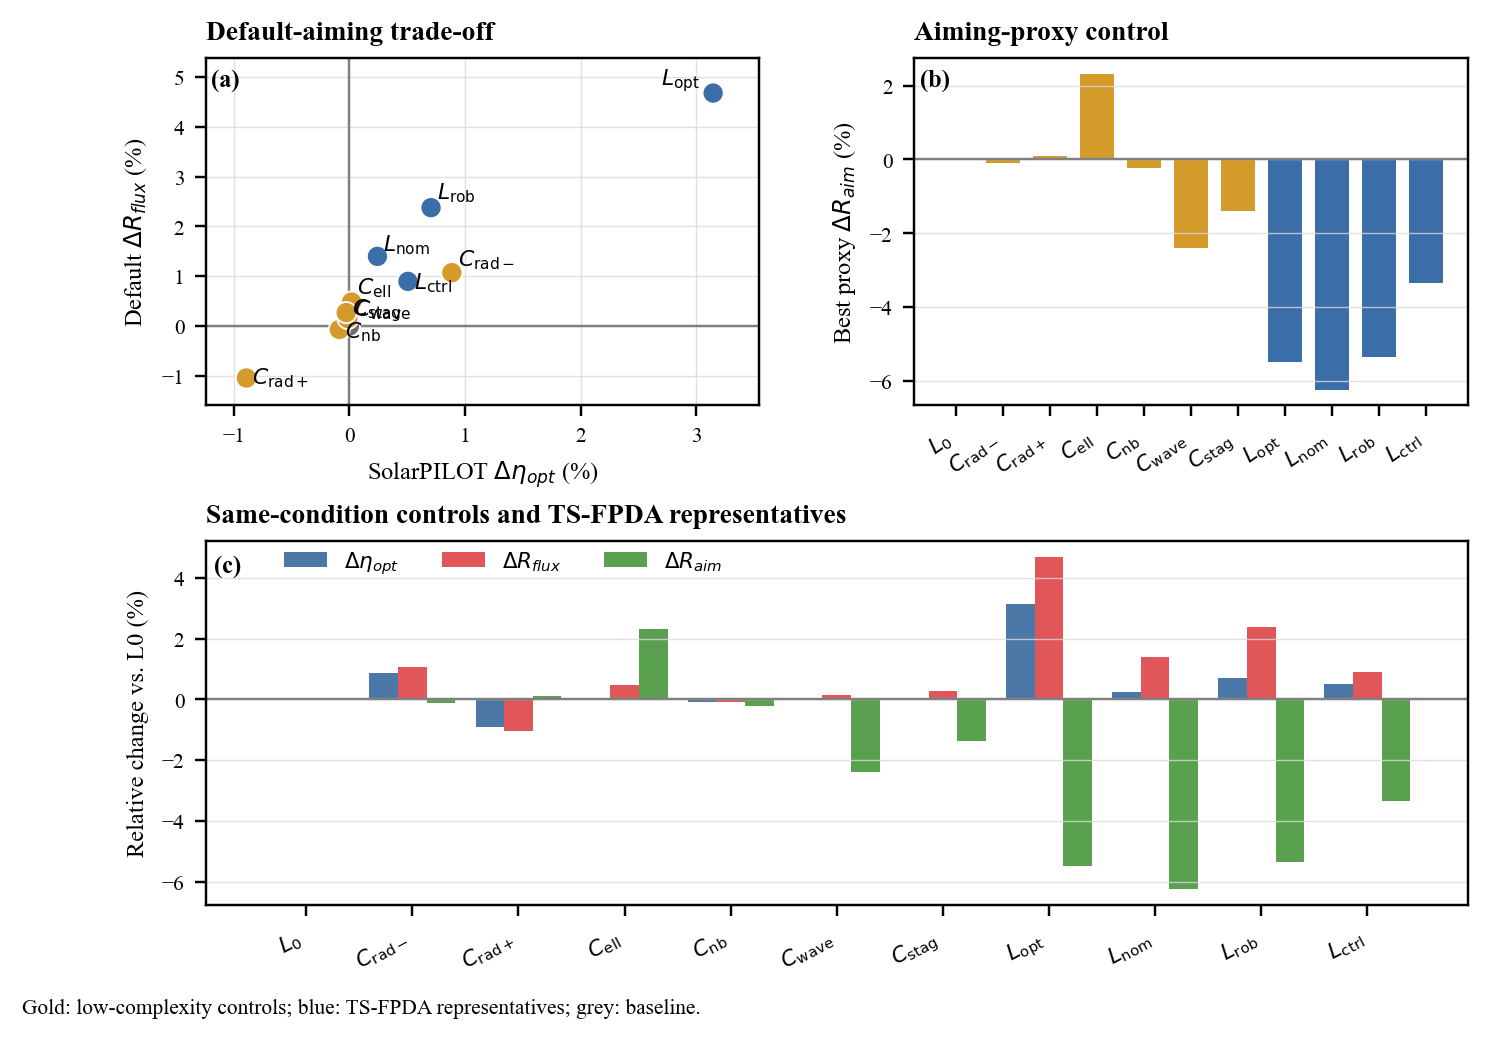
\includegraphics[width=0.92\textwidth]{figures/fig_baseline_controls_summary.png}
\caption{Same-condition baseline-control comparison. Gold marks low-complexity controls, blue marks TS-FPDA representatives, and grey marks the baseline. Panel (a) shows the SolarPILOT default-aiming optical-efficiency and receiver-flux trade-off. Panel (b) compares the best searched aiming-proxy peak-to-mean change. Panel (c) summarizes all three relative metrics against the same $L_0$ baseline.}
\label{fig:baseline-controls}
\end{figure}

\subsection{Same-anchor strong-baseline pressure test}
The low-complexity controls above answer only a limited question: whether one- or two-parameter radial, ellipse, wave, or stagger effects can explain the observed queue. They are not strong enough to address the current layout-optimization literature. A second same-anchor pressure test was therefore added. It generates four literature-inspired approximation families under the same Dunhuang coordinate anchor: a pattern-free approximation with low-frequency sector/ring deformations, a slider-like approximation with ringwise azimuthal shifts, a terrain-aware approximation that responds to public DEM slope/elevation, and a hybrid petal/slider approximation. These families are deliberately labelled as approximations. They are stronger than the simple controls, but they are not complete reproductions of HelioSliders, HeFAAL, modified ABC, or any other named external optimizer.

The pressure test sampled 168 full-field approximation candidates, selected nine representative pressure rows, and then evaluated those rows together with $L_0$, $L_{opt}$, $L_{nom}$, $L_{rob}$, $C_{rad+}$, $J_{bal}$, and $J_{flux}$ using the same SolarPILOT default-aiming bridge and the same aiming-proxy search. This comparison changes the interpretation in a useful way. The TS-FPDA optical upper row remains the strongest default-bridge optical case in the test (+3.15\% SolarPILOT mean optical efficiency), but a hybrid pressure approximation is close enough to matter: $B_{hy,E}$ gives +1.74\% SolarPILOT optical efficiency and -4.44\% best aiming-proxy receiver concentration, while increasing default flux concentration by +1.65\%. Pattern-free and slider-like pressure rows also produce meaningful receiver-proxy reductions: $B_{pf,R}$ gives -5.45\% and $B_{hs,R}$ gives -6.67\% best aiming-proxy changes, but both lose SolarPILOT optical efficiency in this local anchor. The strongest joint row in this same pressure test remains $J_{bal}$ for aiming-proxy reduction (-8.16\%), but its default SolarPILOT flux ratio increases by +1.78\%.

The pressure test changes the interpretation from single-workflow superiority to benchmark discrimination. Stronger local baselines can approach or explain parts of the response, especially the hybrid and slider-like rows, so TS-FPDA should not be read as uniquely discovering all useful geometries. At the same time, the same-anchor test does not erase the role-based queue: $L_{opt}$ remains the optical stress case, $J_{bal}$ and $J_{flux}$ remain joint layout--aiming hypotheses, and the strong-baseline rows become additional candidates for direct promotion. A conservative promotion gate was added after the pressure test to prevent over-writing these screening rows. The gate merges multi-year annual proxy, interpolation robustness, 36-bin SolarPILOT default flux, 12-flux-day sampling, aiming proxy, geometry, and reduced-direct confidence intervals. A completed 27-condition same-run reduced direct follow-up did not promote any new strong-baseline row to a headline direct-supported result: the proxy-selected direct rows for $B_{hy,E}$, $B_{pf,R}$, and $B_{hs,R}$ were adverse or uncertain under the pre-set bootstrap gate, so they remain screening or boundary evidence in the supplementary package. This bounded benchmark claim is the interpretation supported by the current evidence.

\begin{table}[t]
\centering
\caption{Same-anchor strong-baseline pressure test. The baseline families are literature-inspired local approximations under the Dunhuang coordinate anchor, not complete reimplementations of named external optimizers. SolarPILOT values use the common default-aiming bridge; aiming values use the common proxy search.}
\label{tab:strong-baselines}
\scriptsize
\begin{tabular*}{\textwidth}{@{\extracolsep{\fill}}lllrrrp{0.24\textwidth}@{}}
\toprule
Label & Family & Role & $\Delta\eta_{opt}$ (\%) & $\Delta R_{flux}$ (\%) & $\Delta R_{aim}$ (\%) & Interpretation \\
\midrule
$L_{opt}$ & TS-FPDA & optical stress case & +3.15 & +4.68 & -5.48 & Strongest default optical gain; not receiver-safe. \\
$B_{hy,E}$ & hybrid approximation & energy pressure & +1.74 & +1.65 & -4.44 & Strong local baseline; reduces uniqueness of the TS-FPDA optical story. \\
$B_{pf,E}$ & pattern-free approximation & energy pressure & +0.66 & +0.06 & -3.16 & Low flux penalty, moderate proxy benefit. \\
$B_{ta,E}$ & terrain-aware approximation & energy pressure & +1.04 & +1.09 & -0.46 & Terrain-aware pressure row; mainly optical. \\
$B_{hs,E}$ & slider-like approximation & energy pressure & +0.47 & +0.37 & -4.79 & Slider-like baseline with useful proxy response. \\
$J_{bal}$ & joint representative & balance hypothesis & +0.92 & +1.78 & -8.16 & Strongest proxy relief in this table; still needs direct promotion. \\
$B_{hs,R}$ & slider-like approximation & receiver pressure & -0.80 & -0.18 & -6.67 & Receiver-proxy relief with optical loss. \\
$B_{pf,R}$ & pattern-free approximation & receiver pressure & -0.82 & -0.54 & -5.45 & Receiver-proxy relief with optical loss. \\
\bottomrule
\end{tabular*}
\end{table}

\begin{figure}[t]
\centering
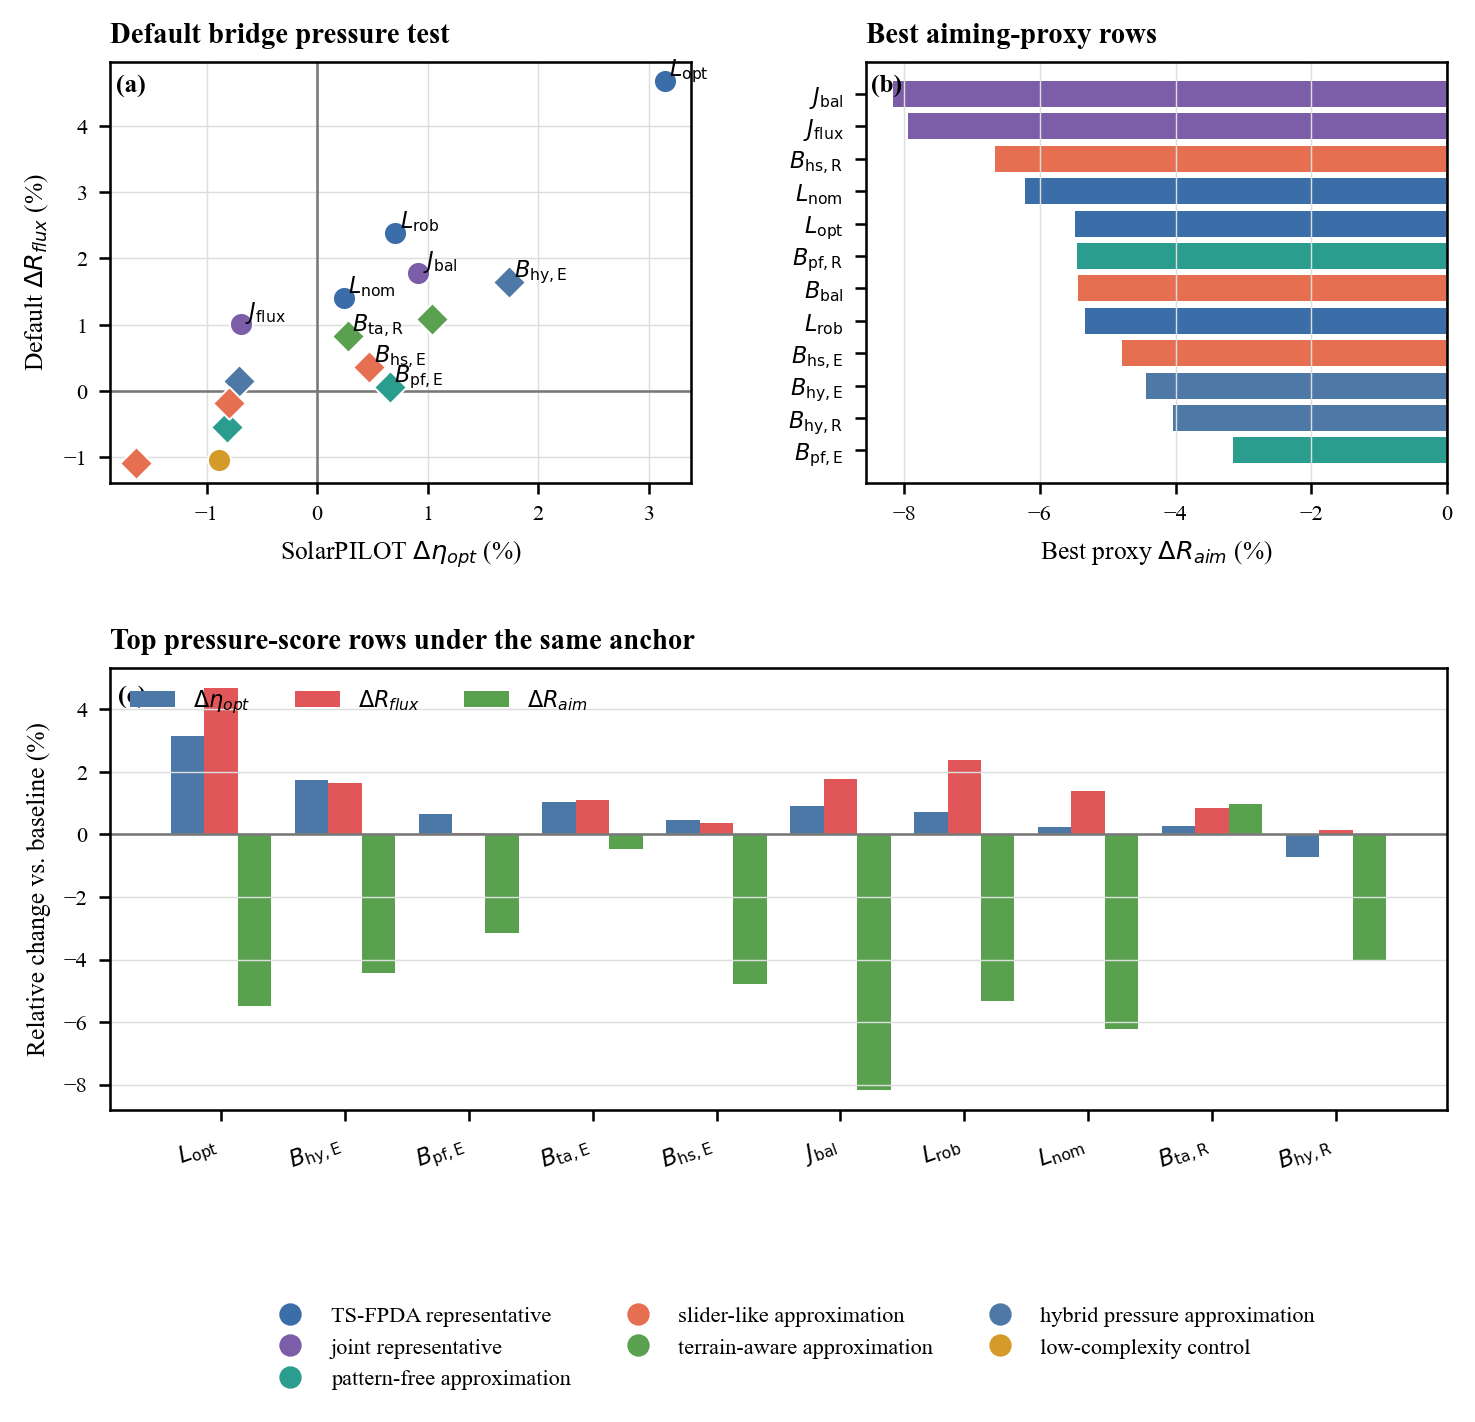
\includegraphics[width=0.92\textwidth]{figures/fig_same_anchor_strong_baselines.png}
\caption{Same-anchor strong-baseline pressure test. Panel (a) compares SolarPILOT default-aiming optical-efficiency change with default receiver-flux concentration change. Panel (b) ranks the strongest best-aiming-proxy rows. Panel (c) shows the top pressure-score rows under the same Dunhuang coordinate anchor. Diamond markers are literature-inspired approximation families; circles are existing TS-FPDA, joint, or control rows.}
\label{fig:strong-baselines}
\end{figure}

\subsection{Geometry explainability and constrained advantage audit}
The strong-baseline pressure test still leaves one practical question: what geometric change is being compared? A visual layout preview can miss small but systematic movement, while a performance table can hide whether a row is a local deformation or a different field concept. A geometry-explainability audit was therefore added for $L_0$, $L_{opt}$, $L_{nom}$, $L_{rob}$, $C_{rad+}$, $J_{bal}$, $J_{flux}$, the hybrid energy row $B_{hy,E}$, and the receiver-pressure rows $B_{pf,R}$ and $B_{hs,R}$. The audit reports radial population shifts, azimuth-sector changes, nearest-neighbour spacing distributions, per-heliostat displacement statistics, and a constrained evidence table that combines fast annual proxy, SolarPILOT default flux, aiming-proxy, AFD-style hotspot-area proxy, and reduced-direct confidence intervals.

The geometry audit supports three bounded conclusions. First, the rows are local count-preserving full-field deformations, not mirror-deletion layouts. $L_{opt}$ has the largest movement scale in the selected set, with mean displacement 58.1 m and p95 displacement 107.5 m, while the receiver-pressure strong-baseline rows move less: $B_{pf,R}$ has p95 displacement 45.4 m and $B_{hs,R}$ has 36.9 m. All selected rows keep nearest-neighbour p05 spacing near or above 16.8 m, and the azimuth-sector L1 population shift remains small, 0.0--2.6\% of the field. Second, the geometry evidence explains why $L_{opt}$ should not be written as a final winner. It is the strongest fast annual optical stress case (+3.36\%) but also has the largest movement scale, default-flux penalty, and AFD-style p99 hotspot-area increase. Third, the constrained table separates evidence roles more clearly than a single ranking can. $L_{nom}$, $L_{rob}$, and $J_{flux}$ are the current direct-supported receiver-risk boundary rows; $J_{bal}$ is an annual-positive balance hypothesis with directional direct support; $B_{hy,E}$ is an annual-positive strong-baseline screening row; and $B_{pf,R}$ and $B_{hs,R}$ are receiver-pressure screening rows whose completed same-run direct follow-up did not clear the promotion gate.

\begin{figure}[t]
\centering
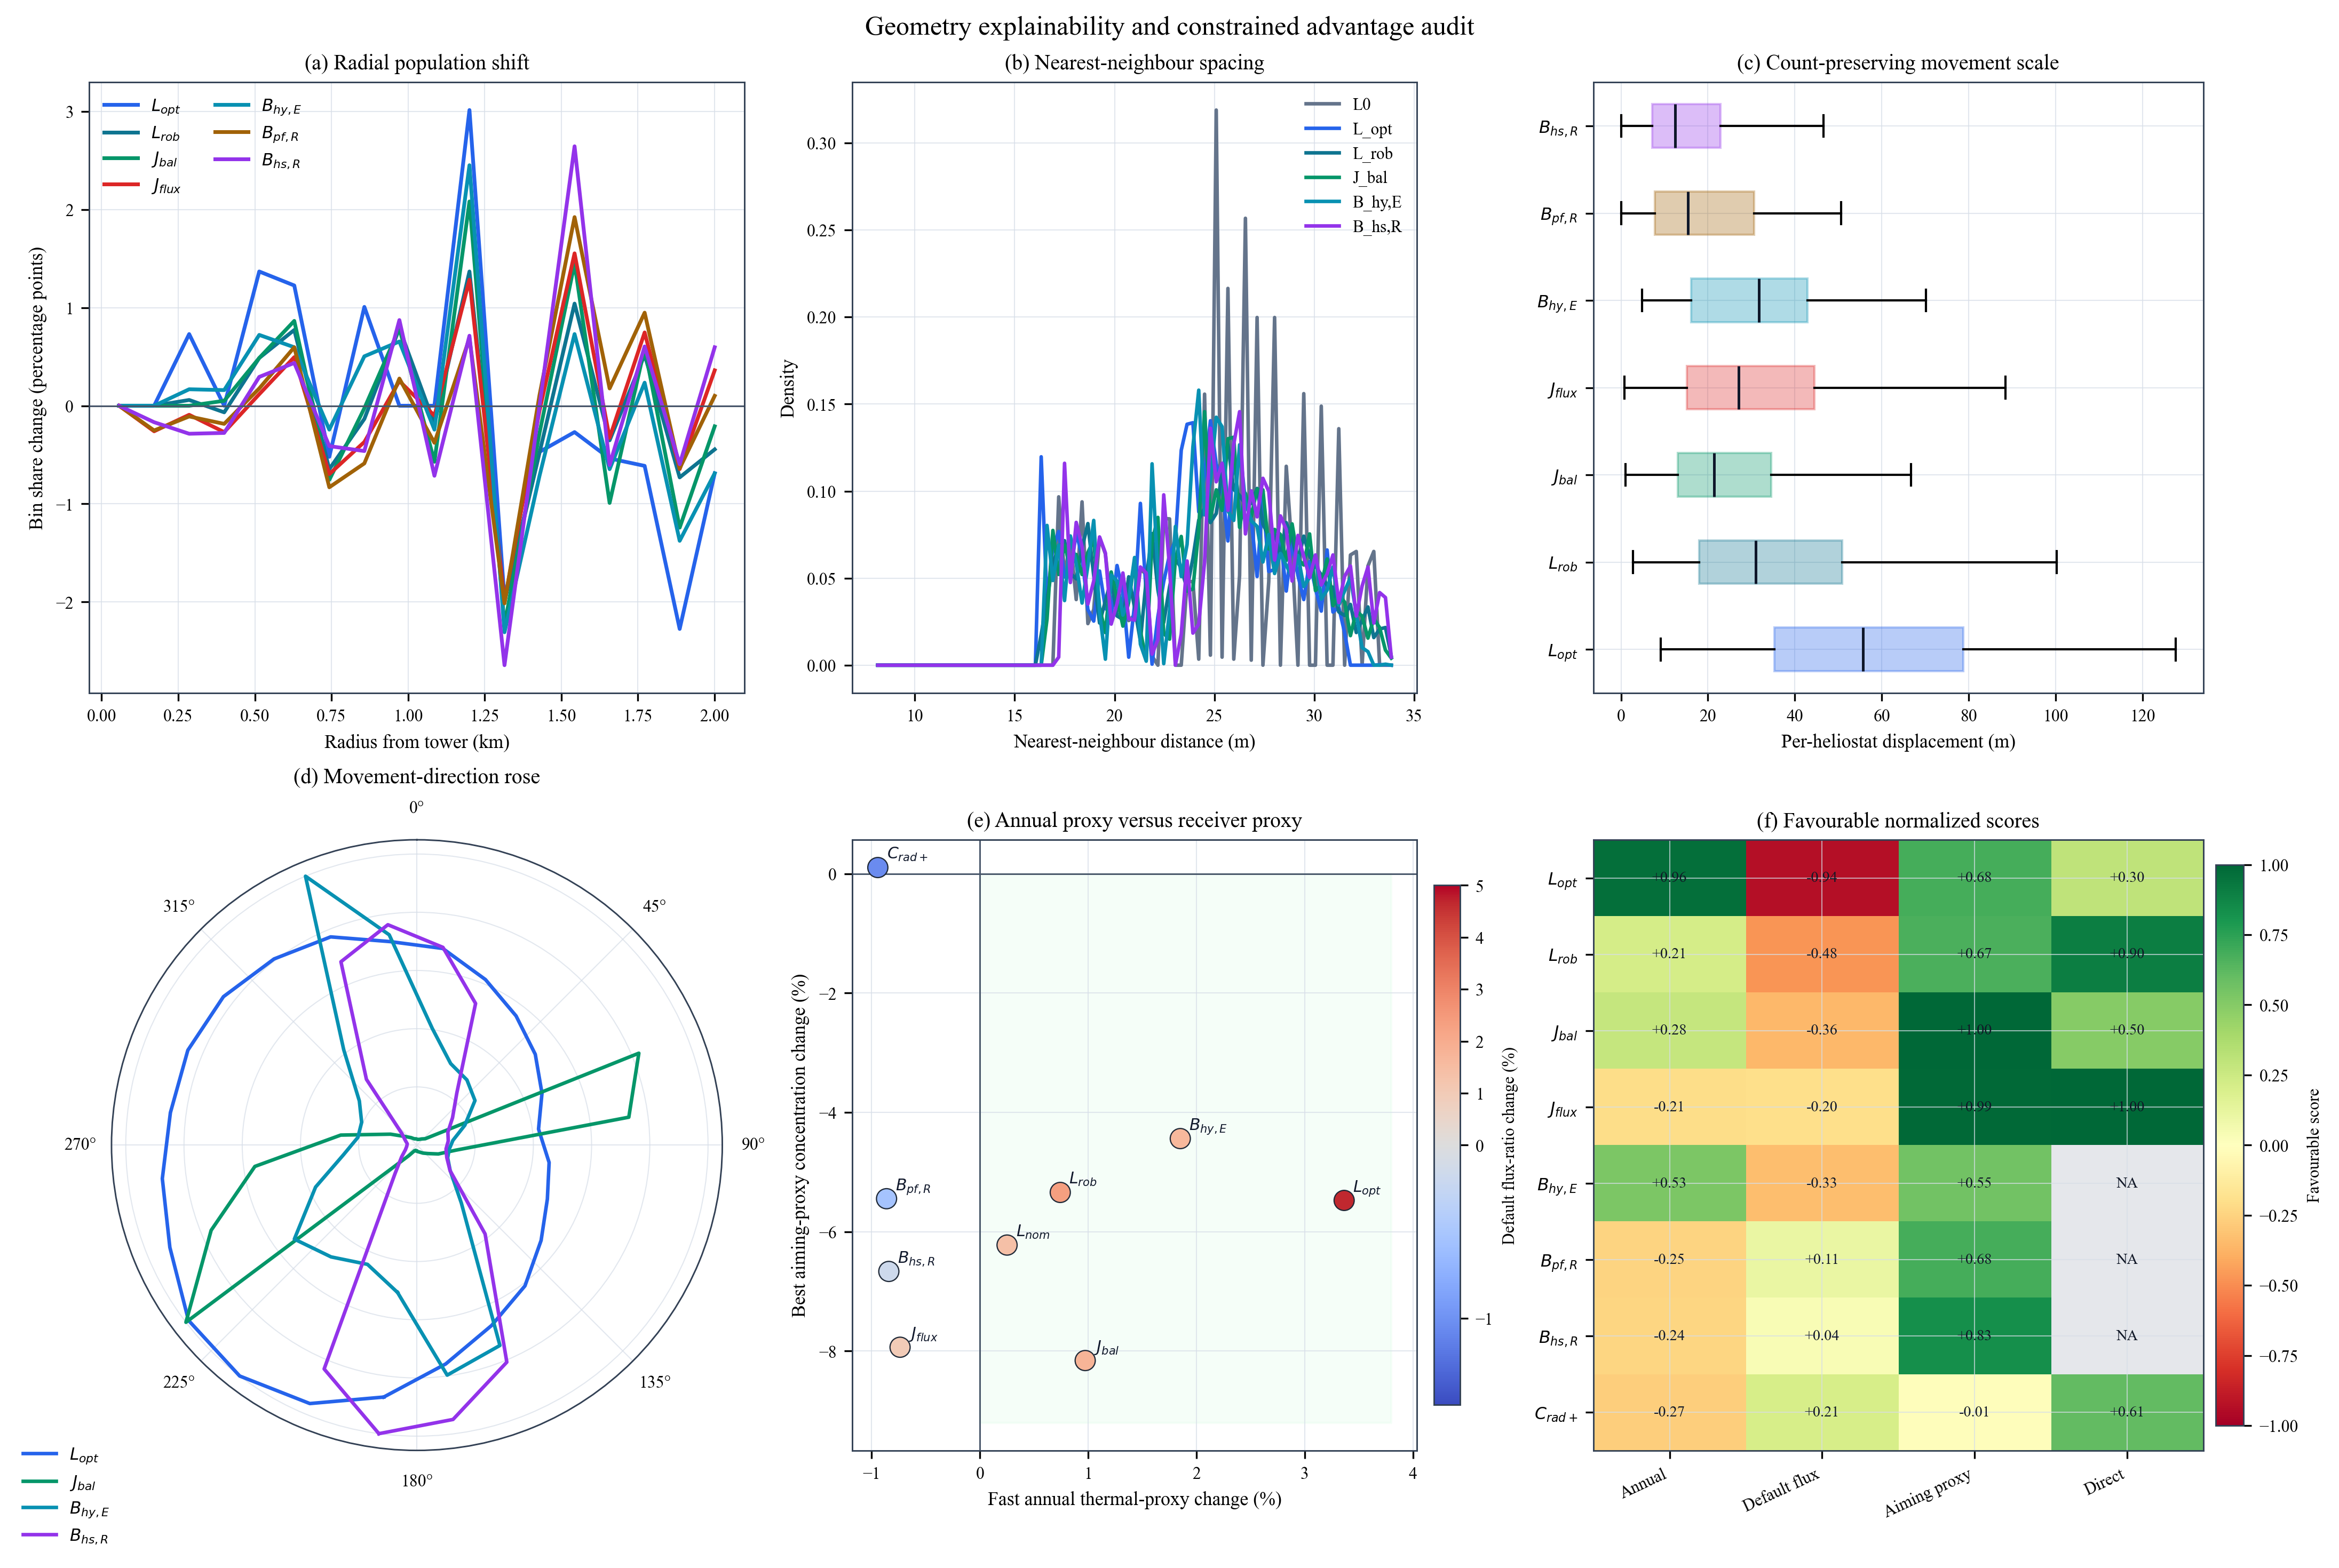
\includegraphics[width=0.96\textwidth]{figures/fig_geometry_explainability_advantage.png}
\caption{Geometry explainability and constrained advantage audit. Panel (a) shows radial population-share changes relative to the baseline. Panel (b) compares nearest-neighbour spacing distributions. Panel (c) reports count-preserving displacement scales for selected rows. Panel (d) shows movement-direction rose curves weighted by displacement magnitude. Panel (e) compares fast annual optical-proxy change with best aiming-proxy receiver concentration; point colour gives the SolarPILOT default-flux penalty. Panel (f) summarizes favourable normalized evidence scores; grey cells mark rows without completed reduced-direct evidence. The figure explains candidate roles and constraints, not a single-method ranking.}
\label{fig:geometry-advantage}
\end{figure}

\subsection{Reduced direct baseline-control audit}
The same-condition controls were also checked with a reduced PySolTrace direct-ray audit, because a proxy-only baseline comparison would still leave the strongest reviewer objection unresolved. This audit uses the baseline, the three most informative simple controls ($C_{rad-}$, $C_{rad+}$, and $C_{wave}$), and the four TS-FPDA representatives. Each layout is traced over the same 27 representative solar conditions with visible-equator aiming, five-point aiming, and five S9 staggered phases. The sampled field size is 6,000 heliostats per layout, with 60,000 requested first-stage ray hits per case, an 18-panel receiver approximation, and 20 by 60 bins per panel. The run contains 1,512 layout--strategy--condition rows and is reported as a reduced direct audit, not as full-field annual certification.

Table~\ref{tab:baseline-direct} gives the useful full-matrix result. The simple controls remain meaningful: $C_{rad+}$ gives a -2.43\% best-direct mean peak-to-active-mean change, and $C_{wave}$ gives -2.30\%. These rows make the evidence more honest by showing that low-complexity geometry already explains part of the receiver-risk response. The TS-FPDA queue is still not redundant, however. $L_{rob}$ gives the strongest direct best-row reduction (-3.61\%) and is the only row in this full-matrix audit whose bootstrap confidence interval remains below zero. $L_{nom}$ is close (-3.49\%) but its interval touches zero. In contrast, the proxy-selected rows are weaker and sometimes adverse: $L_{nom}$ and $L_{opt}$ have positive proxy-selected mean changes in this direct audit. The conclusion is therefore sharper than before. TS-FPDA should be described as a role-level benchmark generator whose candidates require direct checking; it should not be described as a uniformly superior optimizer.

\begin{table}[t]
\centering
\caption{Reduced direct PySolTrace baseline-control audit. Negative values indicate lower peak-to-active-mean receiver concentration than the paired baseline under the same condition and aiming strategy. Bootstrap confidence intervals resample the 27 condition-level deltas.}
\label{tab:baseline-direct}
\scriptsize
\begin{tabular*}{\textwidth}{@{\extracolsep{\fill}}llllrrrr@{}}
\toprule
Layout & Family & Best strategy & Cases & Mean $\Delta R$ (\%) & 95\% CI (\%) & Lower frac. & Proxy-selected mean (\%) \\
\midrule
$C_{rad-}$ & control & S9-p5 & 27 & -1.44 & [-5.03, +2.15] & 0.67 & -0.64 \\
$C_{rad+}$ & control & visible & 27 & -2.43 & [-6.61, +1.70] & 0.56 & -1.20 \\
$C_{wave}$ & control & five-point & 27 & -2.30 & [-5.80, +1.20] & 0.56 & +1.33 \\
$L_{opt}$ & TS-FPDA & five-point & 27 & -1.20 & [-5.80, +3.65] & 0.74 & +1.62 \\
$L_{nom}$ & TS-FPDA & S9-p0 & 27 & -3.49 & [-7.15, +0.09] & 0.52 & +2.11 \\
$L_{rob}$ & TS-FPDA & S9-p2 & 27 & -3.61 & [-6.17, -0.97] & 0.59 & -0.40 \\
$L_{ctrl}$ & TS-FPDA & five-point & 27 & -0.88 & [-4.47, +2.71] & 0.44 & -0.73 \\
\bottomrule
\end{tabular*}
\end{table}

\begin{figure}[t]
\centering
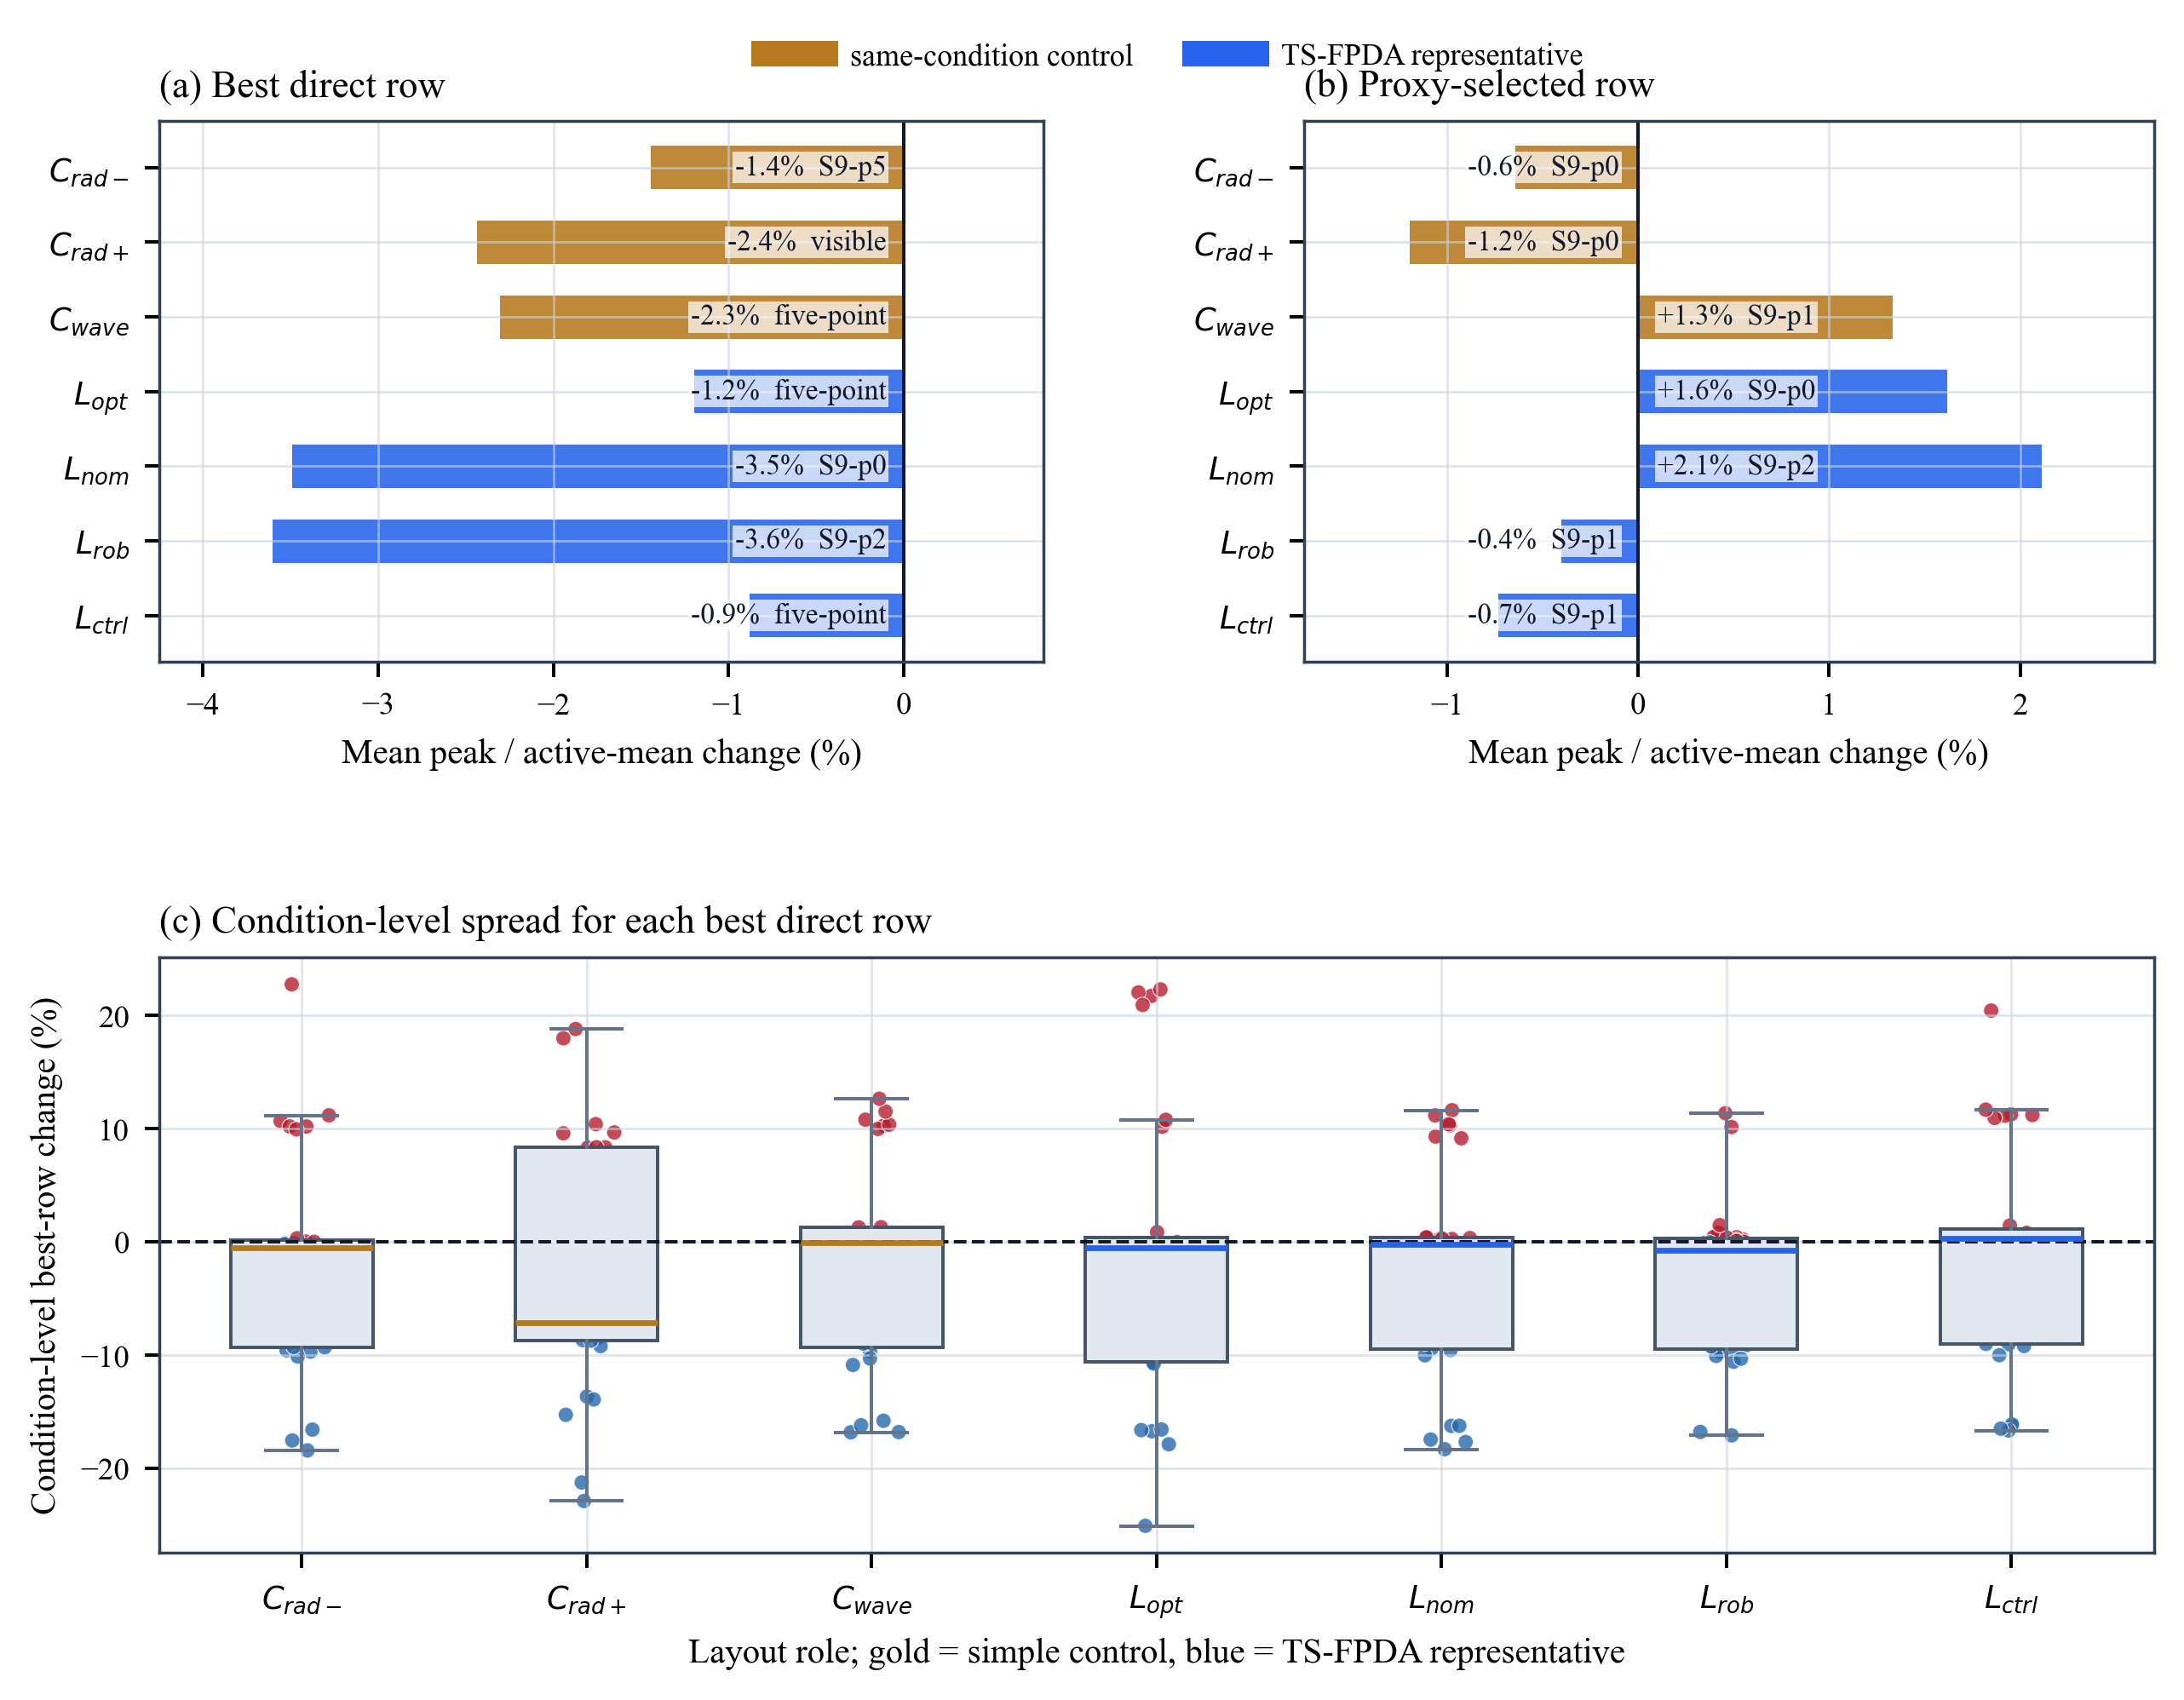
\includegraphics[width=0.92\textwidth]{figures/fig_baseline_direct_soltrace_controls.png}
\caption{Reduced direct PySolTrace baseline-control audit. Panel (a) reports each layout's best direct row among the tested strategies. Panel (b) reports the proxy-selected row under the same direct audit. Panel (c) shows condition-level spread for the best direct row, making clear that several reductions remain condition-dependent.}
\label{fig:baseline-direct}
\end{figure}

The strictest objection to Table~\ref{tab:baseline-direct} is that it selects and reports the best strategy on the same 27-condition matrix. To expose that optimism, a leave-one-day-out audit was added. For each non-baseline layout, one representative day is held out, the best aiming strategy is selected from the other eight days, and the selected strategy is evaluated only on the three held-out hourly conditions. Table~\ref{tab:baseline-direct-holdout} reports the day-level mean changes. The result is narrower and more credible than the full-matrix best-row view: $L_{rob}$ and $L_{nom}$ remain negative with day-bootstrap intervals below zero, while $C_{rad+}$ becomes directional but uncertain and $C_{rad-}$, $C_{wave}$, $L_{opt}$, and $L_{ctrl}$ lose the apparent full-matrix benefit. This audit is not a substitute for annual custom aiming, but it directly reduces the selection-bias risk in the reduced direct layer.

\begin{table}[t]
\centering
\caption{Leave-one-day-out direct-ray strategy-selection audit. For each layout, the best aiming strategy is selected on eight representative days and then evaluated on the held-out day. Confidence intervals bootstrap the nine held-out day means. Negative values indicate lower peak-to-active-mean concentration than the paired baseline.}
\label{tab:baseline-direct-holdout}
\scriptsize
\begin{tabular*}{\textwidth}{@{\extracolsep{\fill}}llrrrrr@{}}
\toprule
Layout & Modal selected strategy & Held-out mean $\Delta R$ (\%) & 95\% CI (\%) & Lower-day frac. & Optimism gap (pct-pt) & Modal share \\
\midrule
$C_{rad-}$ & S9-p5 & +2.08 & [-0.26, +4.75] & 0.33 & +3.52 & 0.78 \\
$C_{rad+}$ & visible & -1.07 & [-4.61, +1.93] & 0.67 & +1.37 & 0.89 \\
$C_{wave}$ & five-point & +1.62 & [-0.45, +4.18] & 0.33 & +3.93 & 0.67 \\
$L_{opt}$ & five-point & +2.41 & [-1.01, +6.21] & 0.44 & +3.61 & 0.78 \\
$L_{nom}$ & S9-p0 & -3.49 & [-5.77, -1.38] & 0.78 & +0.00 & 1.00 \\
$L_{rob}$ & S9-p2 & -3.61 & [-5.19, -1.89] & 0.89 & +0.00 & 1.00 \\
$L_{ctrl}$ & five-point & +3.75 & [+1.23, +6.96] & 0.11 & +4.62 & 0.56 \\
\bottomrule
\end{tabular*}
\end{table}

\subsection{Joint layout--aiming screening}
The baseline-control and hold-out audits make the paper more defensible, but by themselves they are still diagnostic. A further joint layout--aiming screening run was therefore added to test whether the system can actively search for candidates that balance optical contribution and receiver concentration before entering the direct-ray queue. The run evaluated 489 full-field candidates, preserved all 11,915 heliostats in every candidate, tested 23 aiming strategies per candidate, and retained 121 joint Pareto candidates. All candidates passed the publishable-geometry gates.

Table~\ref{tab:joint-optimizer} reports the representative queue selected from this joint layer. The strongest receiver-risk boundary candidate, $J_{flux}$, lowers the best-aiming proxy peak-to-active-mean ratio by 7.22\%, but it also reduces the optical proxy by 0.20\%. This is useful as a Pareto boundary, not as a headline improvement. The more publishable story is the no-energy-loss part of the queue: $J_{bal}$ gives a nearly neutral optical-proxy change (+0.002\%) with a 4.32\% proxy receiver reduction, while $J_{gain}$ gives a +0.091\% optical-proxy change with a 3.47\% proxy receiver reduction. These two candidates are not yet direct-ray results; they are stronger hypotheses for the next verification layer because layout and aiming were selected together.

\begin{table}[t]
\centering
\caption{Joint layout--aiming screening representatives. The changes are proxy-level values from the integrated search loop and are normalized to the same baseline and best searched baseline aiming strategy. Negative $\Delta R_{aim}$ indicates lower proxy peak-to-active-mean receiver concentration.}
\label{tab:joint-optimizer}
\scriptsize
\begin{tabular*}{\textwidth}{@{\extracolsep{\fill}}lllrrrr@{}}
\toprule
Label & Candidate & Role & $\Delta E_{proxy}$ (\%) & $\Delta R_{aim}$ (\%) & $\Delta S_{spill}$ (pct-pt) & Quality \\
\midrule
$J_{flux}$ & \texttt{joint\_g04\_0478} & receiver-risk boundary & -0.195 & -7.222 & +0.002 & 0.991 \\
$J_{bal}$ & \texttt{joint\_g02\_0333} & no-energy-loss balance & +0.002 & -4.316 & -0.024 & 0.973 \\
$J_{gain}$ & \texttt{joint\_g02\_0303} & energy-gated receiver candidate & +0.091 & -3.468 & -0.010 & 0.965 \\
$J_{Emax}$ & \texttt{joint\_g00\_0097} & maximum energy with receiver gate & +0.134 & -0.075 & +0.000 & 0.970 \\
$J_{spill}$ & \texttt{joint\_g01\_0254} & minimum spillage diagnostic & -0.091 & +0.930 & -0.037 & 1.000 \\
\bottomrule
\end{tabular*}
\end{table}

\begin{figure}[t]
\centering
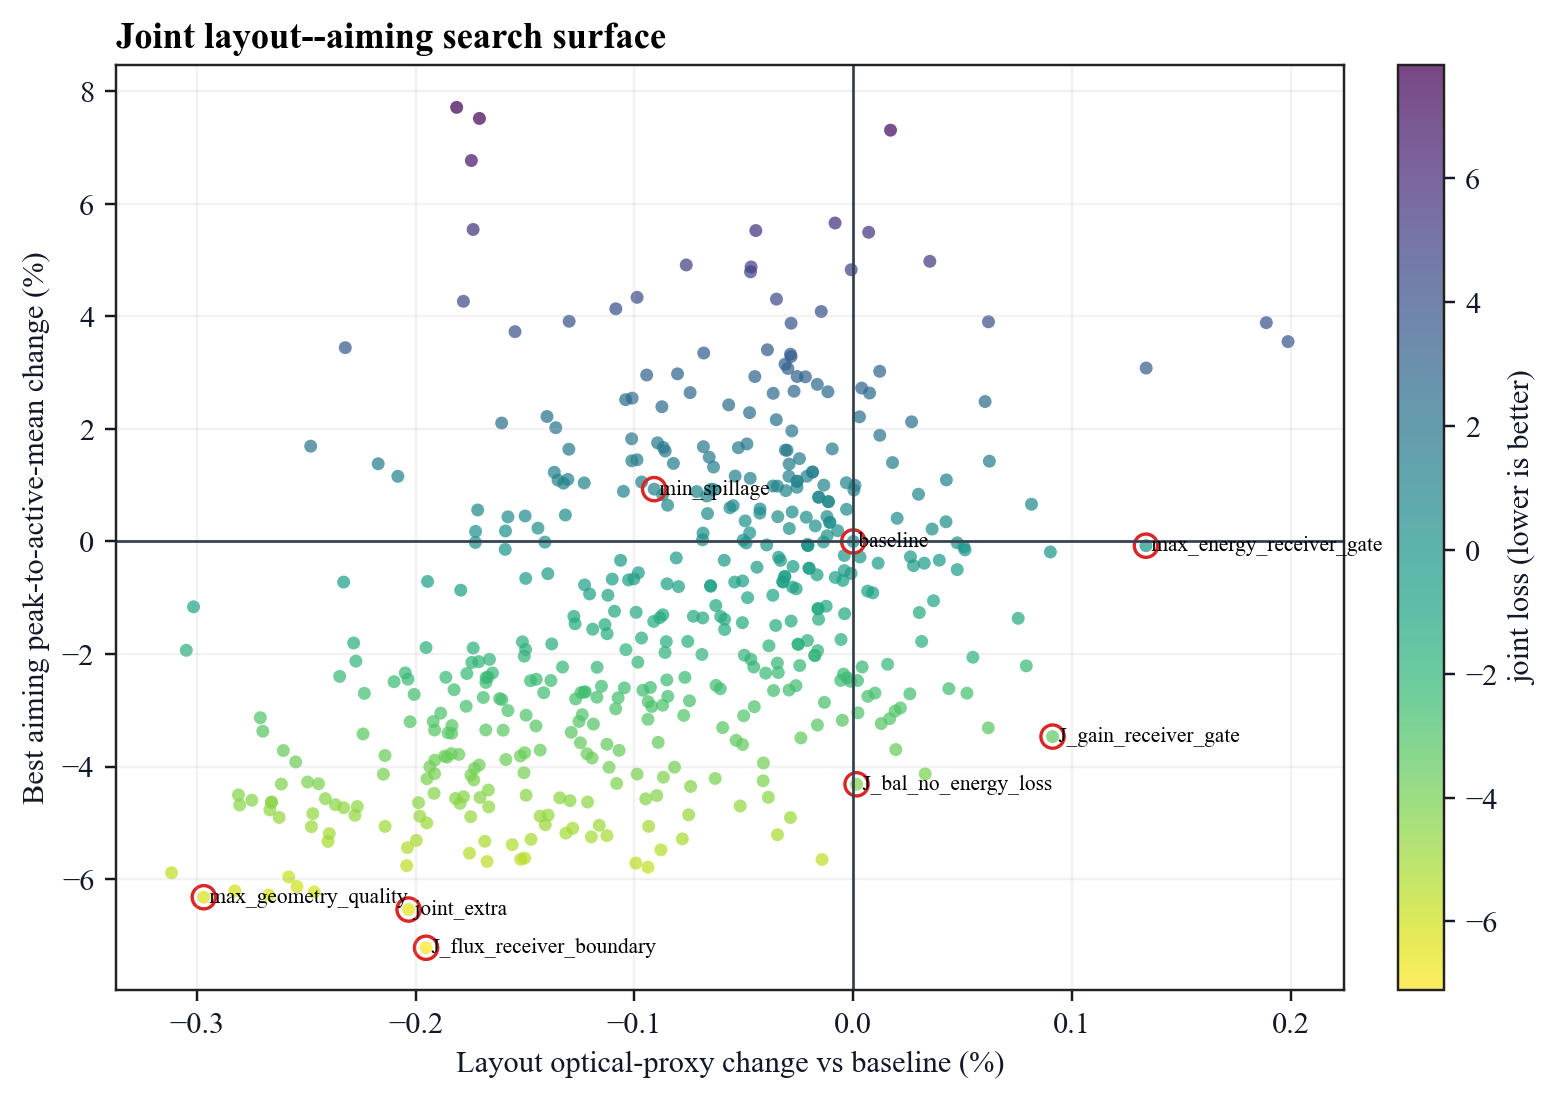
\includegraphics[width=0.88\textwidth]{figures/fig_joint_optimizer_pareto.png}
\caption{Joint layout--aiming screening surface. Each point is a full-field layout deformation evaluated with its best searched aiming strategy. The highlighted representatives separate receiver-risk boundary, no-energy-loss balance, and energy-gated receiver candidates. The figure is used as a screening result; the selected representatives are being promoted to reduced direct ray-tracing checks before any direct receiver-risk claim is made.}
\label{fig:joint-optimizer}
\end{figure}

Figure~\ref{fig:joint-optimizer-convergence} shows that the elite-mutation search improved the best joint-loss and receiver proxy over successive generations. This convergence is useful evidence that the joint layer is doing more than replaying the original representative table. However, the loss function is still a screening device. The paper therefore treats $J_{bal}$ and $J_{gain}$ as candidates to be audited with reduced direct ray tracing, not as final plant-design recommendations.

\begin{figure}[t]
\centering
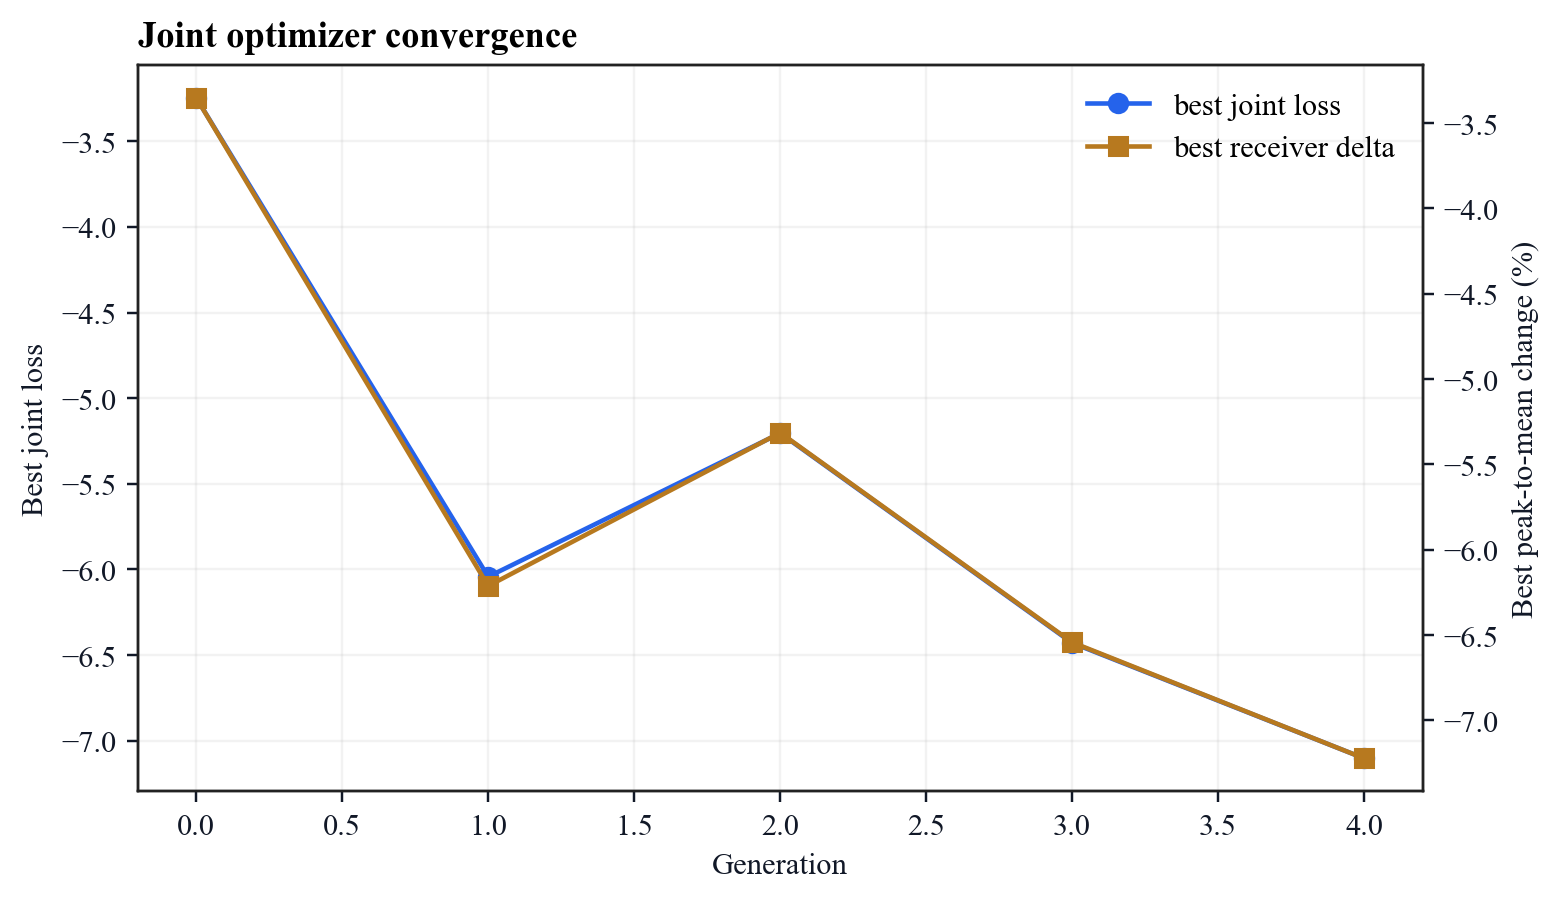
\includegraphics[width=0.82\textwidth]{figures/fig_joint_optimizer_convergence.png}
\caption{Convergence of the joint layout--aiming screening run. The best joint-loss and best receiver-proxy reduction improve after the seeded initial population, indicating that the elite-mutation loop is exploring useful local deformations.}
\label{fig:joint-optimizer-convergence}
\end{figure}

\subsection{Joint SolarPILOT bridge}
The joint candidates were also imported into the same PySAM/SolarPILOT default-aiming bridge used for the earlier representatives. This bridge does not test custom aimpoints; it tests whether the joint layouts remain optically plausible under the common SolarPILOT settings before the direct custom-aimpoint promotion layer. Table~\ref{tab:joint-system-evidence} combines the three useful evidence layers for the joint representatives: proxy-level joint screening, SolarPILOT default-aiming layout checking, and reduced PySolTrace direct promotion.

The bridge adds an important nuance. $J_{bal}$ and $J_{gain}$ are not only proxy-energy artifacts: under SolarPILOT default aiming, they increase mean optical efficiency by +0.92\% and +1.64\%, respectively. They also increase the default peak-to-active-mean receiver ratio by +1.78\% and +2.40\%, so their publishable interpretation still depends on custom aiming and direct checking. $J_{flux}$ is the opposite boundary case. It reduces the receiver ratio in the direct audit but loses optical efficiency in both the proxy layer and the SolarPILOT bridge. This three-layer comparison is why the manuscript describes roles and promotion gates instead of declaring a single optimum.

\begin{table}[t]
\centering
\caption{Joint layout--aiming evidence summary across proxy screening, SolarPILOT default-aiming bridge, and reduced direct promotion. SolarPILOT values are relative to the same baseline under default aiming; direct values are paired peak-to-active-mean changes with bootstrap intervals over 27 solar conditions.}
\label{tab:joint-system-evidence}
\scriptsize
\begin{tabular*}{\textwidth}{@{\extracolsep{\fill}}llrrrrp{0.24\textwidth}@{}}
\toprule
Candidate & Role & Proxy $\Delta E$ (\%) & Proxy $\Delta R$ (\%) & SolarPILOT $\Delta\eta$ (\%) & SolarPILOT $\Delta R_{flux}$ (\%) & Direct-promotion interpretation \\
\midrule
$J_{bal}$ & balance & +0.002 & -4.32 & +0.92 & +1.78 & Directional: S9-p2 gives -1.98\% mean, 95\% CI [-6.55,+3.10]\%. \\
$J_{gain}$ & energy-gated & +0.091 & -3.47 & +1.64 & +2.40 & Strategy-sensitive: proxy-selected S9-p3 is adverse; best-direct S9-p2 gives -2.49\% mean but CI crosses zero. \\
$J_{flux}$ & receiver boundary & -0.195 & -7.22 & -0.69 & +1.01 & Promoted as receiver-boundary: S9-p5 gives -4.06\% mean, 95\% CI [-6.99,-0.94]\%. \\
\bottomrule
\end{tabular*}
\end{table}

\subsection{Joint direct promotion audit}
The joint representatives were then promoted to a reduced direct PySolTrace audit. This is the first place where the new joint layer is judged by an optical engine rather than by its internal proxy. The audit compares the baseline, $J_{bal}$, $J_{gain}$, and $J_{flux}$ over the same 27 representative solar conditions used in the baseline-control direct audit. Each condition uses 6,000 sampled heliostats per layout, 60,000 requested first-stage ray hits, an 18-panel receiver approximation, and 20 by 60 bins per panel. The tested strategies are visible-equator aiming, five-point aiming, and S9 phases p2, p3, and p5. This creates 540 direct layout--strategy--condition rows and is still a reduced promotion audit, not a full annual custom-aiming proof.

Table~\ref{tab:joint-direct} gives the manuscript-facing result. The receiver-boundary candidate $J_{flux}$ is promoted by this direct layer: its proxy-selected S9-p5 row also gives the best direct row, with a -4.06\% mean peak-to-active-mean change, a 95\% bootstrap interval from -6.99\% to -0.94\%, and a lower-peak fraction of 0.74. This is not a final prescription because $J_{flux}$ had a small optical-proxy loss in Table~\ref{tab:joint-optimizer}, but it is a direct-supported boundary point. $J_{bal}$ remains directionally useful rather than confirmed: its S9-p2 row gives a -1.98\% mean direct change and a 0.70 lower-peak fraction, but the confidence interval crosses zero. $J_{gain}$ is the most instructive negative result. Its proxy-selected S9-p3 row is adverse in the direct audit (+2.58\% mean), while a different direct row, S9-p2, is directionally lower (-2.49\%) but uncertain. The joint layer therefore improves the system architecture, but it must be coupled to a direct promotion gate.

\begin{table}[t]
\centering
\caption{Reduced direct promotion audit for the joint layout--aiming representatives. Negative values indicate lower peak-to-active-mean receiver concentration than the paired baseline under the same condition and strategy. Confidence intervals bootstrap the 27 condition-level deltas.}
\label{tab:joint-direct}
\scriptsize
\begin{tabular*}{\textwidth}{@{\extracolsep{\fill}}lllrrrrp{0.22\textwidth}@{}}
\toprule
Candidate & View & Strategy & Cases & Mean $\Delta R$ (\%) & 95\% CI (\%) & Lower frac. & Interpretation \\
\midrule
$J_{bal}$ & proxy/best direct & S9-p2 & 27 & -1.98 & [-6.55, +3.10] & 0.70 & Directional balance candidate; not statistically promoted. \\
$J_{gain}$ & proxy selected & S9-p3 & 27 & +2.58 & [-1.67, +6.66] & 0.48 & Proxy-selected phase fails the direct gate. \\
$J_{gain}$ & best direct & S9-p2 & 27 & -2.49 & [-6.74, +2.04] & 0.63 & Directional but strategy-sensitive candidate. \\
$J_{flux}$ & proxy/best direct & S9-p5 & 27 & -4.06 & [-6.99, -0.94] & 0.74 & Direct-supported receiver-boundary candidate. \\
\bottomrule
\end{tabular*}
\end{table}

\begin{figure}[t]
\centering
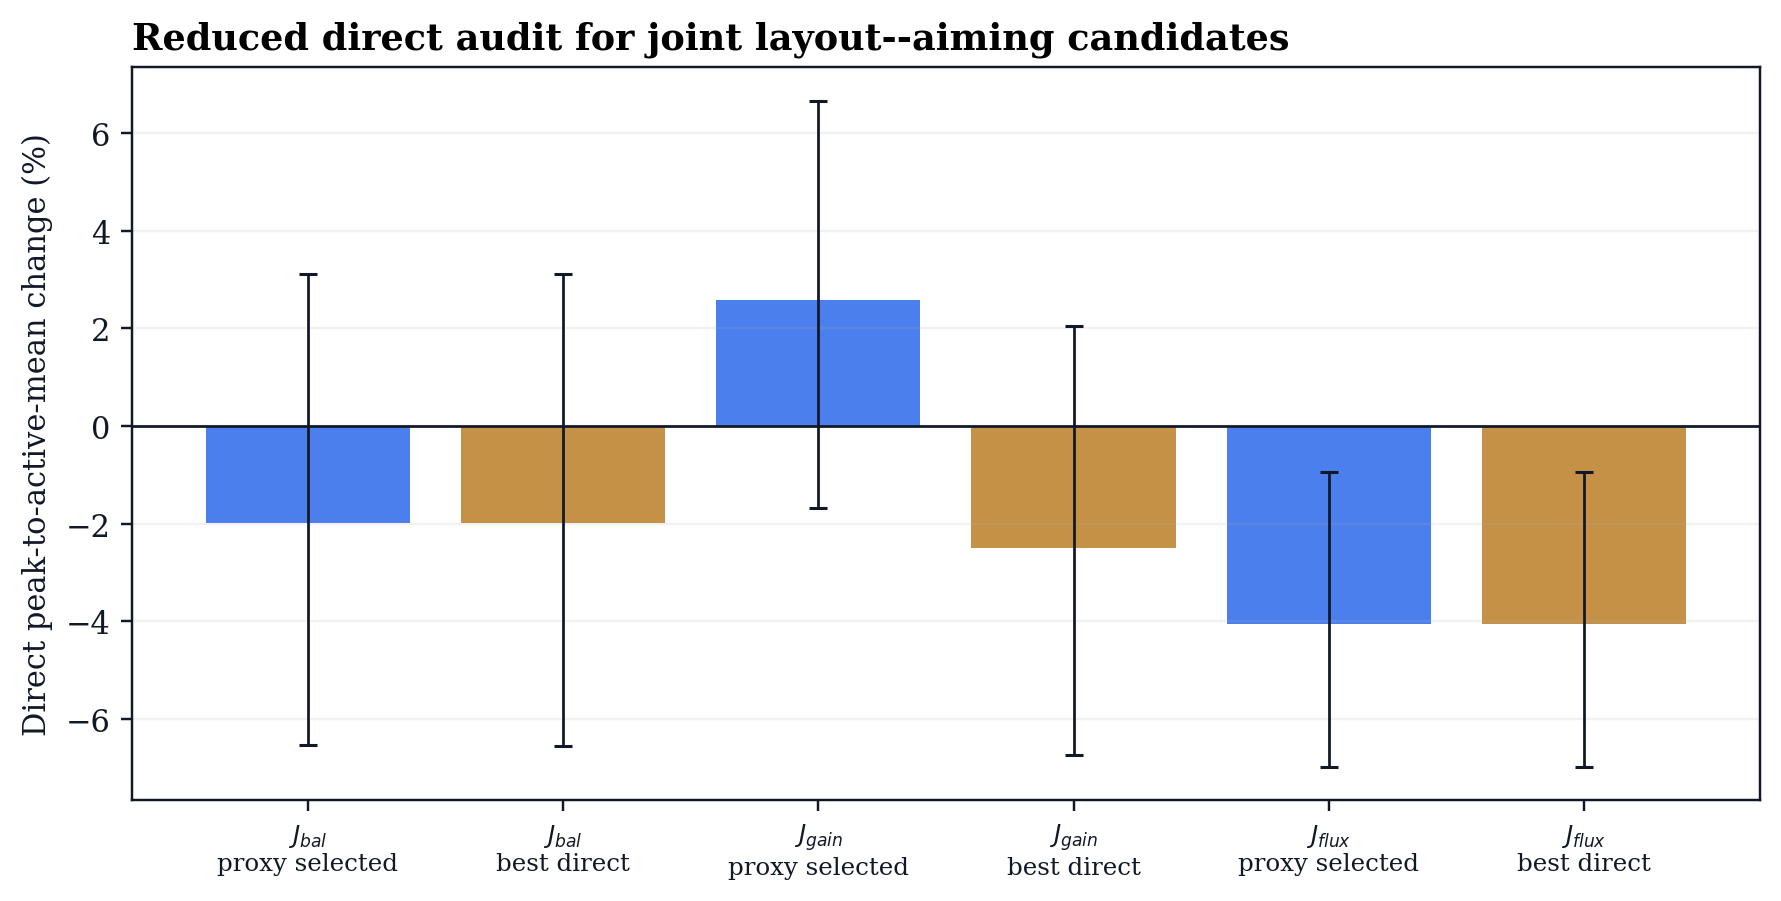
\includegraphics[width=0.86\textwidth]{figures/fig_joint_direct_summary.png}
\caption{Reduced direct promotion audit for the joint layout--aiming representatives. Bars show mean paired changes in peak-to-active-mean receiver concentration, and whiskers show 95\% bootstrap confidence intervals over the 27 representative solar conditions. The plot separates proxy-selected rows from best-direct rows so that strategy mismatch is visible.}
\label{fig:joint-direct}
\end{figure}
\FloatBarrier

\subsection{SolarPILOT default-aiming trade-off}
Table~\ref{tab:summary} and Fig.~\ref{fig:tradeoff} summarize the key result. The optical upper case is not automatically the safest receiver-flux layout. The optical-upper layout $L_{opt}$ improves SolarPILOT mean optical efficiency by 3.15\% but increases default peak-to-active-mean receiver flux by 4.68\%. The nominal proxy layout $L_{nom}$ gives a much smaller default optical gain of 0.24\% and still increases default flux concentration by 1.40\%, but it gives the strongest nominal proxy reduction under the initially searched staggered aiming strategy. The default-flux-control layout $L_{ctrl}$ is a conservative comparison case, with a 0.51\% optical gain and a 0.90\% default-flux increase. These results sharpen the manuscript's main point: layout-only gains remain coupled to receiver loading and must be evaluated with aiming.

This is the main finding at the current verification level. The optical-upper layout cannot be interpreted as unconditionally superior because the optical-efficiency gain is accompanied by a receiver-flux penalty. Any operational value would depend on aimpoint redistribution and receiver thermal constraints. Conversely, the more balanced candidates are informative because their smaller optical gains define the cases where custom-aimpoint checking may be most useful. The result is therefore a documented trade-off rather than a single positive-performance claim.

\begin{table}[t]
\centering
\caption{Integrated numerical-checking summary for representative layouts. Optical and default-flux changes are from PySAM/SolarPILOT. Aiming peak-to-mean change is proxy-screened and is not a final SolarPILOT custom-aimpoint claim. The internal triage score is shown only to disclose representative selection and is not used as a headline result.}
\label{tab:summary}
\scriptsize
\begin{tabular}{lrrrrr}
\toprule
Layout & Role & $\Delta\eta_{opt}$ (\%) & $\Delta R_{flux}$ (\%) & $\Delta R_{aim}$ (\%) & Triage score \\
\midrule
$L_{opt}$ & optical upper & +3.15 & +4.68 & -5.48 & 0.937 \\
$L_{rob}$ & proxy flux-risk & +0.71 & +2.38 & -5.34 & 0.958 \\
$L_{ctrl}$ & default-flux control & +0.51 & +0.90 & -3.33 & 0.992 \\
$L_{nom}$ & nominal proxy & +0.24 & +1.40 & -6.22 & 1.000 \\
$L_0$ & baseline control & +0.00 & +0.00 & +0.00 & 1.000 \\
\bottomrule
\end{tabular}
\end{table}

\begin{figure}[t]
\centering
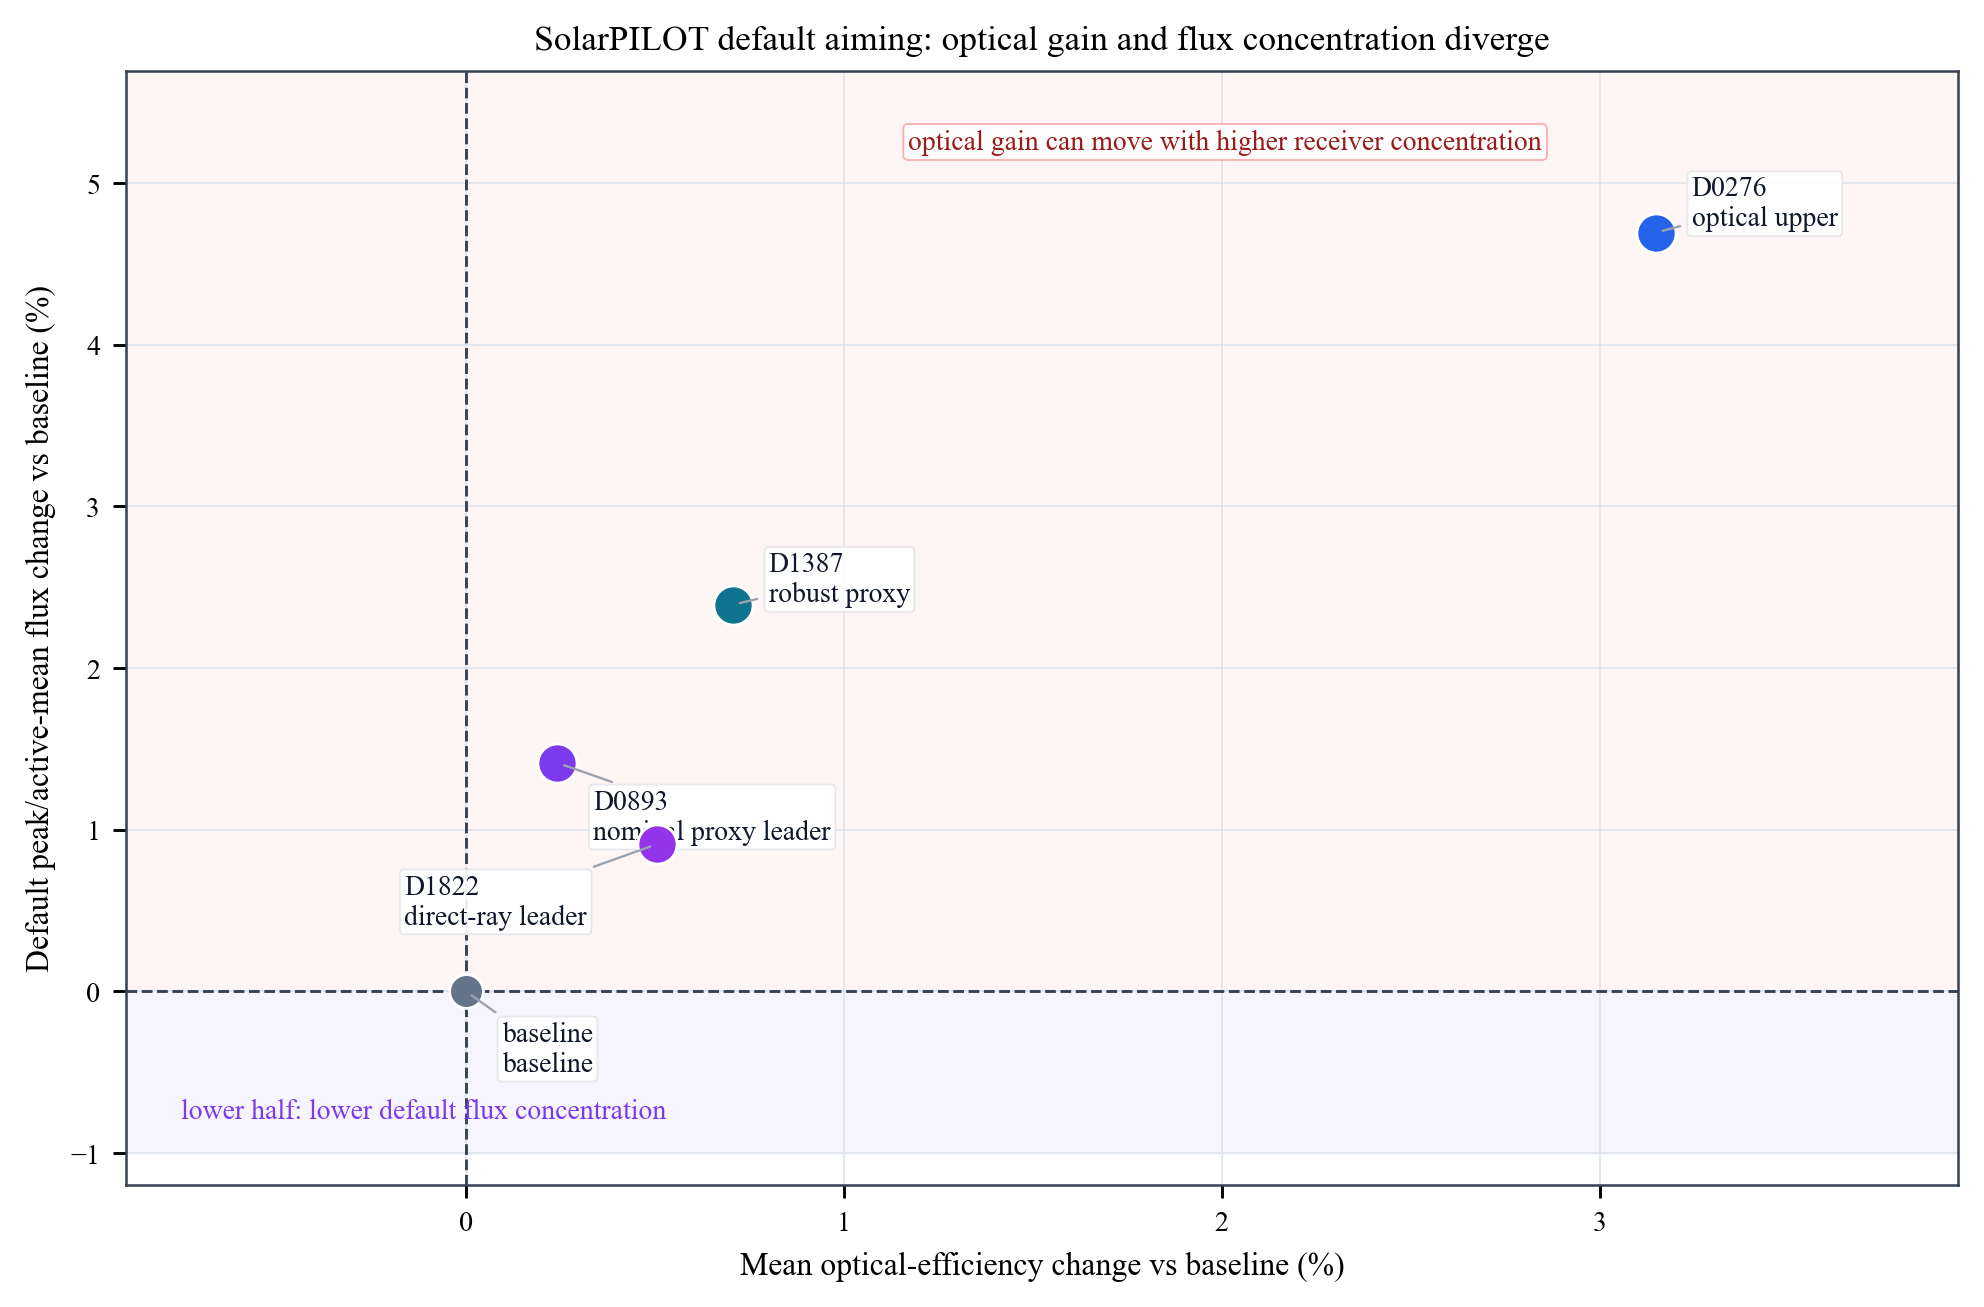
\includegraphics[width=0.78\textwidth]{figures/fig_journal_tradeoff_clean.png}
\caption{SolarPILOT default-aiming trade-off between optical-efficiency change and peak-to-active-mean receiver-flux change. Optical gains are accompanied by higher default flux concentration for the strongest optical candidates.}
\label{fig:tradeoff}
\end{figure}

\subsection{Fast annual proxy and public plant sanity check}
The default-aiming SolarPILOT tables were annualized with a conservative proxy to address whether the representative-condition optical signal is consistent with the public weather year and with the reported Dunhuang plant scale. The proxy interpolates each \path{opteff_*.csv} table over the 8760-hour NASA POWER 2023 weather file, weights daylight hours by DNI, and computes an aperture-based annual thermal input
\begin{equation}
E_{th,proxy}=\sum_t \frac{\mathrm{DNI}_t A_{ap}\eta_{opt}(\alpha_t,\zeta_t)}{10^6},
\end{equation}
where $A_{ap}=11915\times115.72$ m\textsuperscript{2}, $\alpha_t$ and $\zeta_t$ are the approximate solar azimuth and zenith at hour $t$, and the annual DNI is uniformly scaled from the public NASA POWER value of 1842.4 kWh m\textsuperscript{-2} y\textsuperscript{-1} to the 1883 kWh m\textsuperscript{-2} y\textsuperscript{-1} corrected typical-year DNI reported for Dunhuang. This is not a dispatch model, SAM annual simulation, or custom-aimpoint annual ray trace. Its role is to test whether the default optical ranking is an artifact of a few representative SolarPILOT positions.

The fast annual proxy preserves the main optical ranking. The optical-upper case $L_{opt}$ remains the strongest annualized optical row, with a +3.36\% annual thermal-proxy change relative to $L_0$. The strongest same-anchor hybrid energy row gives +1.85\%, and $J_{bal}$ gives +0.97\%. The baseline annual thermal proxy is 945.9 GWh\textsubscript{th} under the corrected-DNI scaling. Matching the 351.6 GWh design annual generation reported in the public plant paper requires a net electric conversion factor of 0.372, while the same reference corresponds to a 40.14\% capacity factor for a 100 MW plant. This places the proxy in the right plant-scale order, but it does not make any candidate a bankable annual-yield result.

A multi-year weather-robustness gate then repeated the same annualization over the available 2020--2025 NASA POWER SAM files. Annual DNI varied from 1694.9 to 2012.4 kWh m\textsuperscript{-2} y\textsuperscript{-1}, but the selected role signs did not change. $L_{opt}$ stayed rank 1 in all six years, $B_{hy,E}$ stayed rank 2, and the annual-positive rows $J_{bal}$, $L_{rob}$, and $L_{nom}$ remained positive in every year. The receiver-pressure rows $J_{flux}$, $B_{pf,R}$, and $B_{hs,R}$ remained negative annual-proxy rows, so they were not promoted into annual headline candidates. This audit is included in \path{supplementary_data/multiyear_annual_proxy_gate/}; it supports weather-year sign and rank stability, not annual custom-aimpoint validation. The annualized proxy therefore reinforces the existing conclusion: the best optical rows should remain stress cases because their receiver-flux penalties persist in the default-aiming and AFD-style audits.

An additional interpolation-robustness gate tested whether this annual-proxy ranking depends on the single inverse-distance interpolation used in the first annualization. The audit repeated the 2020--2025 public-weather calculation with nearest-neighbour, IDW-3, IDW-6, IDW-12, and linear interpolation with nearest fallback. Across all tested method-year pairs, $L_{opt}$ remained rank 1, $B_{hy,E}$ remained rank 2, $J_{bal}$, $L_{rob}$, and $L_{nom}$ remained positive, and the receiver-pressure rows remained non-headline annual rows. The largest selected annual-delta spread was 0.197 percentage points, just below the pre-set 0.20 percentage-point gate. The result is stored in \path{supplementary_data/annual_interpolation_robustness_gate/}; it supports interpolation robustness of the annual proxy, not measured annual operation.

\begin{figure}[t]
\centering
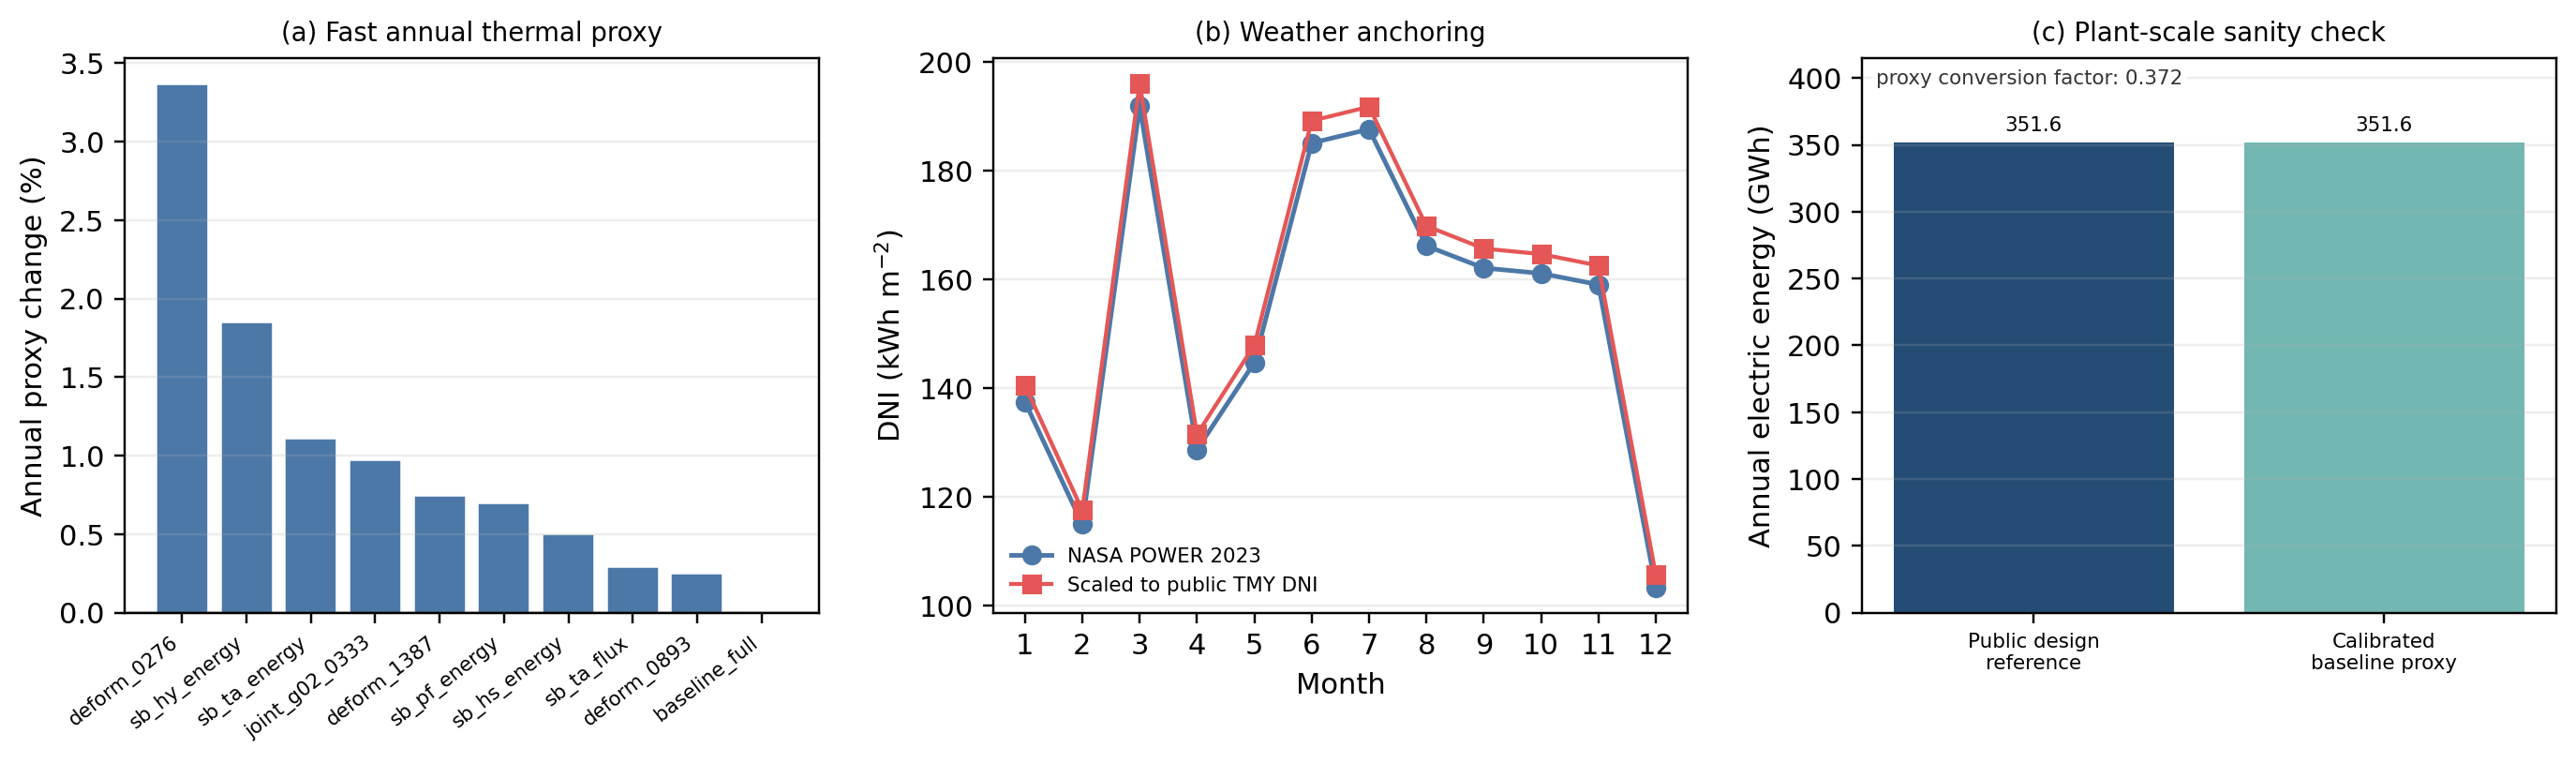
\includegraphics[width=0.94\textwidth]{figures/fig_fast_annual_proxy_sanity.png}
\caption{Fast annual proxy and public plant sanity check. Panel (a) annualizes the SolarPILOT optical-efficiency tables over the 8760-hour public weather file after DNI scaling to the reported Dunhuang corrected typical-year value. Panel (b) compares the NASA POWER monthly DNI profile with the uniformly scaled profile. Panel (c) checks the baseline proxy against the public 351.6 GWh design-generation reference through a calibrated net electric conversion factor. The figure is an annualization and plant-scale sanity bridge, not a full annual custom-aimpoint or dispatch validation.}
\label{fig:fast-annual-proxy}
\end{figure}

\subsection{Deformation-component ablation}
The deformation family is not treated as an uninterpretable black box. Table~\ref{tab:ablation} summarizes a component-ablation experiment for the optical upper case $L_{opt}$ and the nominal aiming-proxy leader $L_{nom}$. The proxy ablation decomposes each candidate into scale, radial/north-bias, twist/wave, and petal terms. A light SolarPILOT numerical checking run then imports the same ablated coordinates with \path{flux-days = 2} and \path{flux-bins = 16}. This lower-resolution run is used only to diagnose component effects; the headline performance claims remain based on the high-resolution numerical check in Table~\ref{tab:summary}.

For $L_{opt}$, removing the scale terms reduces the quick SolarPILOT optical gain from 2.80\% to 1.14\%, while removing radial/north terms gives 1.75\%. This indicates that the optical upper case is driven mainly by field-scale and radial redistribution rather than by an isolated decorative petal term. Removing the twist/wave terms leaves the optical gain nearly unchanged but reduces the quick default-flux penalty from 3.90\% to 3.56\%, showing that the same terms that shape the field can also alter receiver loading.

For $L_{nom}$, the ablation is more cautionary. The proxy indicates that twist/wave terms are important for its low flux-risk index, but quick SolarPILOT default-flux changes do not follow the proxy ranking exactly. This mismatch is useful evidence: the proxy is effective as a candidate funnel, but final receiver-risk interpretation must come from SolarPILOT, CoPylot, SolTrace, or another optical engine.

\begin{table}[t]
\centering
\caption{Component-ablation diagnostics. Proxy metrics come from the screening model; quick SolarPILOT changes are relative to the same quick baseline and are used only for component interpretation.}
\label{tab:ablation}
\scriptsize
\begin{tabular*}{\textwidth}{@{\extracolsep{\fill}}lrrrr@{}}
\toprule
Variant & Proxy $E/E_0$ & Proxy flux & Quick $\Delta\eta_{opt}$ (\%) & Quick $\Delta R_{flux}$ (\%) \\
\midrule
\texttt{d0276}: full & 1.002037 & 0.986 & +2.80 & +3.90 \\
\texttt{d0276}: no scale & 1.000812 & 0.990 & +1.14 & +1.71 \\
\texttt{d0276}: no radial/north & 1.001323 & 0.987 & +1.75 & +2.32 \\
\texttt{d0276}: no twist/wave & 1.002100 & 0.993 & +2.85 & +3.56 \\
\texttt{d0893}: full & 0.999706 & 0.979 & +0.14 & +1.42 \\
\texttt{d0893}: no scale & 1.000208 & 0.978 & +0.56 & +1.51 \\
\texttt{d0893}: no north bias & 0.999677 & 0.976 & +0.08 & +1.37 \\
\texttt{d0893}: no twist/wave & 0.999884 & 0.996 & +0.17 & +1.10 \\
\bottomrule
\end{tabular*}
\end{table}

\subsection{Resolution stability of SolarPILOT numerical verification}
The quick and high-resolution SolarPILOT runs lead to the same qualitative ranking for the main candidates. $L_{opt}$ remains the optical upper case in both settings; $L_{ctrl}$ remains the lowest default-flux-penalty non-baseline candidate among the high-resolution set; and $L_{nom}$ remains a small-gain layout whose main value is the custom-aimpoint queue. The high-resolution run increases the measured optical gain of $L_{opt}$ from 2.80\% to 3.15\% and increases its default-flux penalty from 3.90\% to 4.68\%. These differences are not large enough to change the interpretation, but they justify using the high-resolution run for all headline claims.

A second discretization gate compared the existing 24 by 24 SolarPILOT receiver-flux tables with a 36 by 36 rerun for the direct-promotion queue layouts. The high-resolution rerun preserved the default-flux role labels. The maximum absolute shift in peak-to-active-mean delta was 0.43 percentage points, and the maximum absolute shift in p99-to-active-mean delta was 0.18 percentage points. $L_{opt}$ still carried a positive high-resolution flux penalty (+5.00\% peak-to-active-mean and +0.36\% p99-to-active-mean), while the receiver-pressure rows did not become annual or default-flux headline winners. The detailed comparison is stored in \path{supplementary_data/flux_resolution_gate/}. This gate reduces the risk that the receiver-flux interpretation is an artifact of one coarse receiver-map discretization, but it remains a SolarPILOT default-aiming check rather than receiver thermal certification.

A third SolarPILOT sampling gate enlarged the flux-map sampling from the original 8 flux days to 12 flux days for the same selected direct-promotion layouts. The rerun produced 130 default receiver maps per layout and again preserved the role interpretation. Relative to the original 8-day tables, the maximum absolute shift in peak-to-active-mean delta was 0.008 percentage points and the maximum p99-to-active-mean shift was 0.073 percentage points. $L_{opt}$ still carried a 12-day default-flux penalty (+4.69\% peak-to-active-mean), and the receiver-pressure rows did not become optical headline rows. The result is stored in \path{supplementary_data/flux_day_sampling_gate/}. Like the receiver-bin gate, it is a default-aiming robustness check, not annual custom aiming or receiver thermal certification.

\subsection{Weather and DNI anchoring}
The SolarPILOT numerical check uses a public NASA POWER 2023 weather file because it is reproducible. This choice is checked against the public Dunhuang plant report rather than left implicit. The NASA POWER file gives an annual DNI of 1842.4 kWh m\textsuperscript{-2} y\textsuperscript{-1}, while the reported corrected typical-year DNI for the plant is 1883 kWh m\textsuperscript{-2} y\textsuperscript{-1}. The corresponding uniform scale factor is 1.022. This difference is small enough that the relative optical-efficiency and peak-to-active-mean rankings are not an artifact of an obviously mismatched weather file.

Uniform DNI scaling does not change the relative SolarPILOT optical-efficiency changes or the peak-to-active-mean receiver-flux ratios in Table~\ref{tab:summary}; it changes only the absolute flux scale under the same optical geometry. For example, the high-resolution $L_0$ peak value scales from 0.003200 to 0.003271 in the exported flux-table units, while $L_{opt}$ scales from 0.003362 to 0.003436. The flux-ratio penalty of $L_{opt}$ therefore remains approximately 4.68\%. The weather check supports the robustness of the relative trade-off interpretation, but it is not a substitute for a measured TMY or plant-grade weather file.

\subsection{Receiver-flux normalization and thermal-safety interpretation}
The receiver-flux evidence in this manuscript is intentionally reported as a relative numerical-checking metric. SolarPILOT exports flux tables under a common receiver discretization, weather file, heliostat area, optical-error setting, and default-aiming policy; within that common setup, the peak-to-active-mean ratio is useful because it shows whether a layout concentrates power more strongly on the receiver than the baseline. It is not, by itself, a certified molten-salt receiver heat-flux limit.

A thermal-safety interpretation would require calibrated absorbed-power density, for example
\begin{equation}
q''_{peak}=\max_j(P_j/A_j), \qquad
q''_{mean,active}=\frac{\sum_{j\in\mathcal{A}}P_j}{\sum_{j\in\mathcal{A}}A_j},
\end{equation}
where $P_j$ is absorbed thermal power assigned to receiver cell $j$, $A_j$ is the corresponding cell area, and $\mathcal{A}$ is the active illuminated receiver set. Converting the current exported flux-table values into publishable kW m\textsuperscript{-2} or MW m\textsuperscript{-2} limits would require plant-specific absorptance, tube-panel thermal limits, receiver-control policy, defocus rules, measured or plant-grade DNI, heliostat optical calibration, and a consistent receiver thermal model. Those data are not available in the public package. The manuscript therefore uses $R_{flux}=q''_{peak}/q''_{mean,active}$ as a conservative screening ratio and treats absolute receiver heat-flux certification as a required next-stage experiment, not as a hidden assumption.

To reduce the risk of relying on one peak/mean number, the SolarPILOT flux tables were also converted into a relative AFD-style proxy audit. The audit keeps the same default-aiming bridge and computes active-zone p95 and p99 concentration, the fraction of active receiver cells above the baseline p99 threshold, and mean excess above baseline high-percentile thresholds. It is still a relative screening layer, because the thresholds come from the baseline numerical flux table rather than from an allowable tube-flux standard. The useful result is that it agrees with the main trade-off without overstating thermal safety. $L_{opt}$ improves default optical efficiency by 3.15\% but increases the active p99 hotspot-area proxy by 0.38 percentage points. In contrast, $L_{rob}$ and $L_{ctrl}$ reduce that default-aiming hotspot-area proxy by 0.23 and 0.16 percentage points, respectively, while the joint default-aiming bridge gives -0.27 percentage points for $J_{flux}$ and -0.13 percentage points for $J_{bal}$. These values support the receiver-risk screening interpretation, but they do not replace the reduced direct custom-aimpoint audits or a future receiver thermal model.

\begin{figure}[t]
\centering
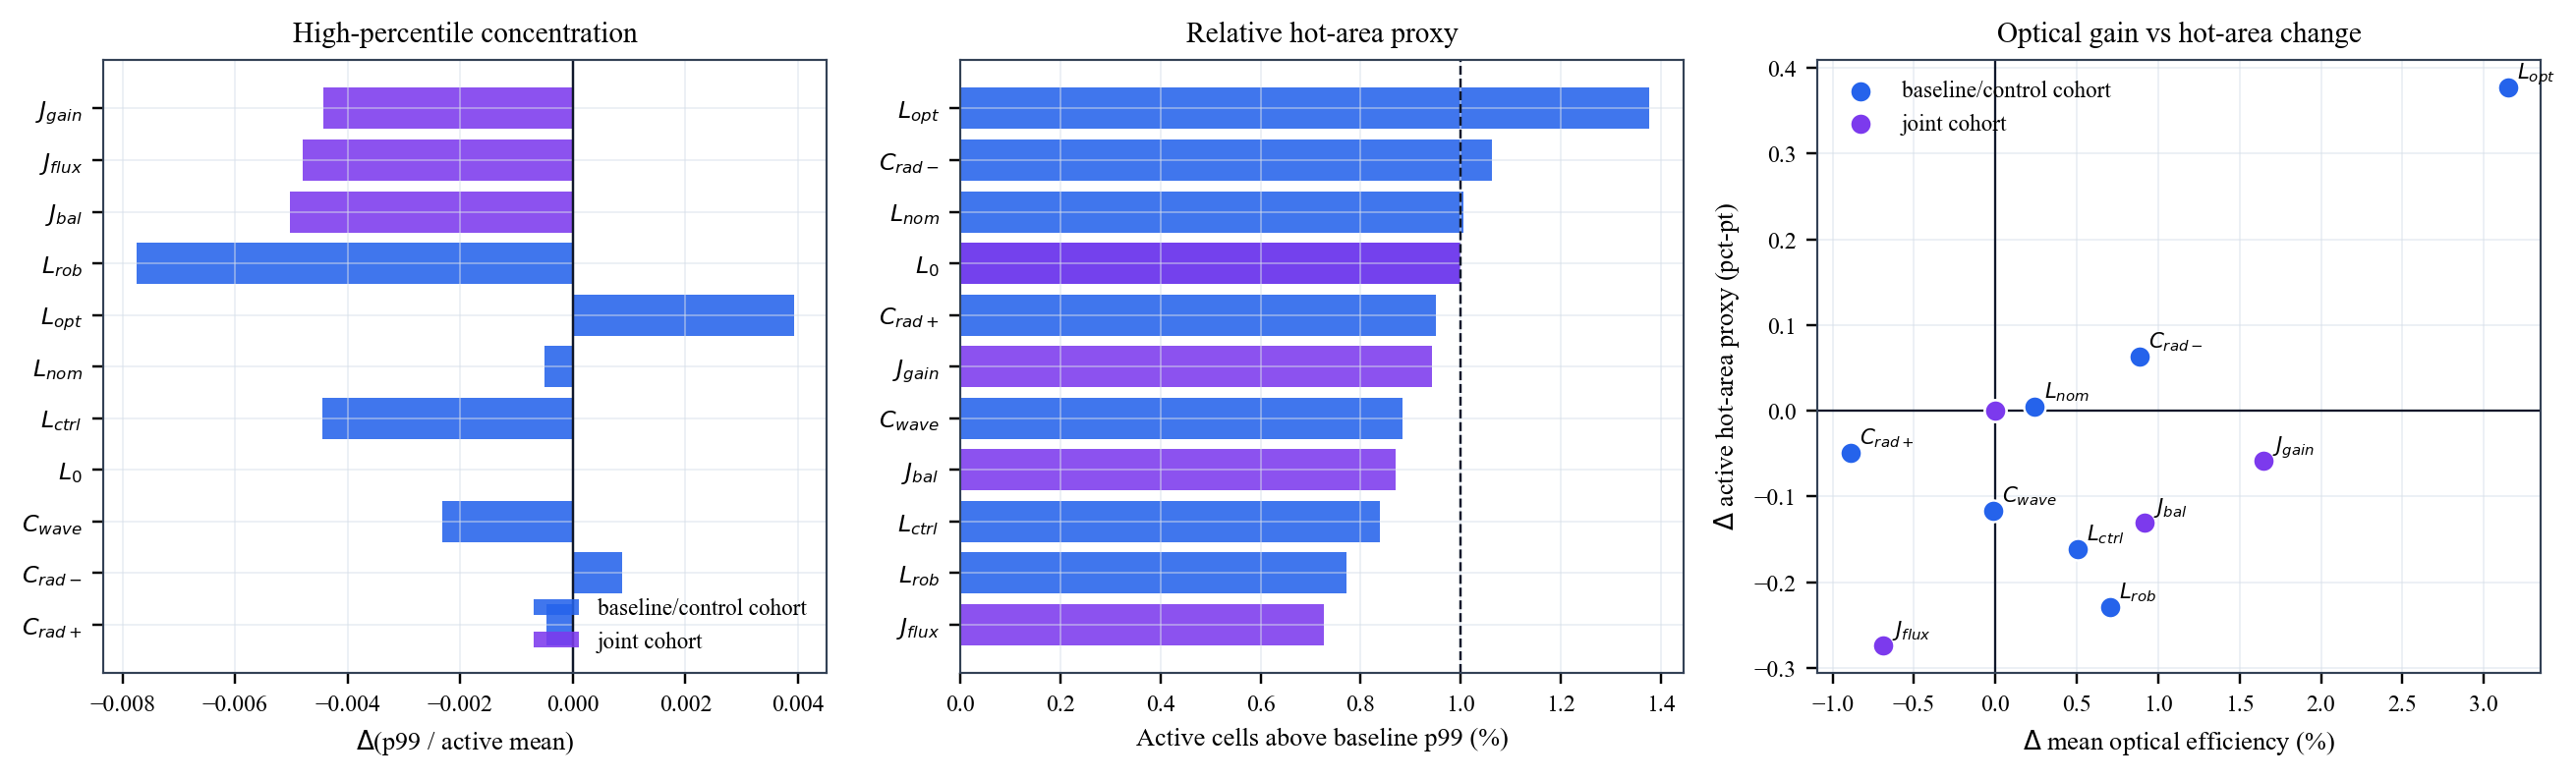
\includegraphics[width=0.94\textwidth]{figures/fig_afd_style_flux_proxy.png}
\caption{Relative AFD-style receiver-flux proxy audit derived from the SolarPILOT default-aiming flux tables. Panel (a) reports changes in active-zone p99 concentration. Panel (b) reports the fraction of active cells above the baseline p99 threshold. Panel (c) compares mean optical-efficiency change with the active p99 hotspot-area proxy. The thresholds are baseline-relative numerical thresholds, not allowable receiver-tube heat-flux limits.}
\label{fig:afd-proxy}
\end{figure}

\subsection{Receiver-flux maps}
Figure~\ref{fig:fluxmaps} shows peak-flux snapshots under the same color scale. The maps provide qualitative evidence that layout changes alter receiver loading patterns even when the field envelope remains visually similar. They also explain why final layout--aiming claims require custom aiming: default aiming creates comparable high-flux regions, whereas distributed aiming may change the receiver-risk ranking.

\begin{figure}[t]
\centering
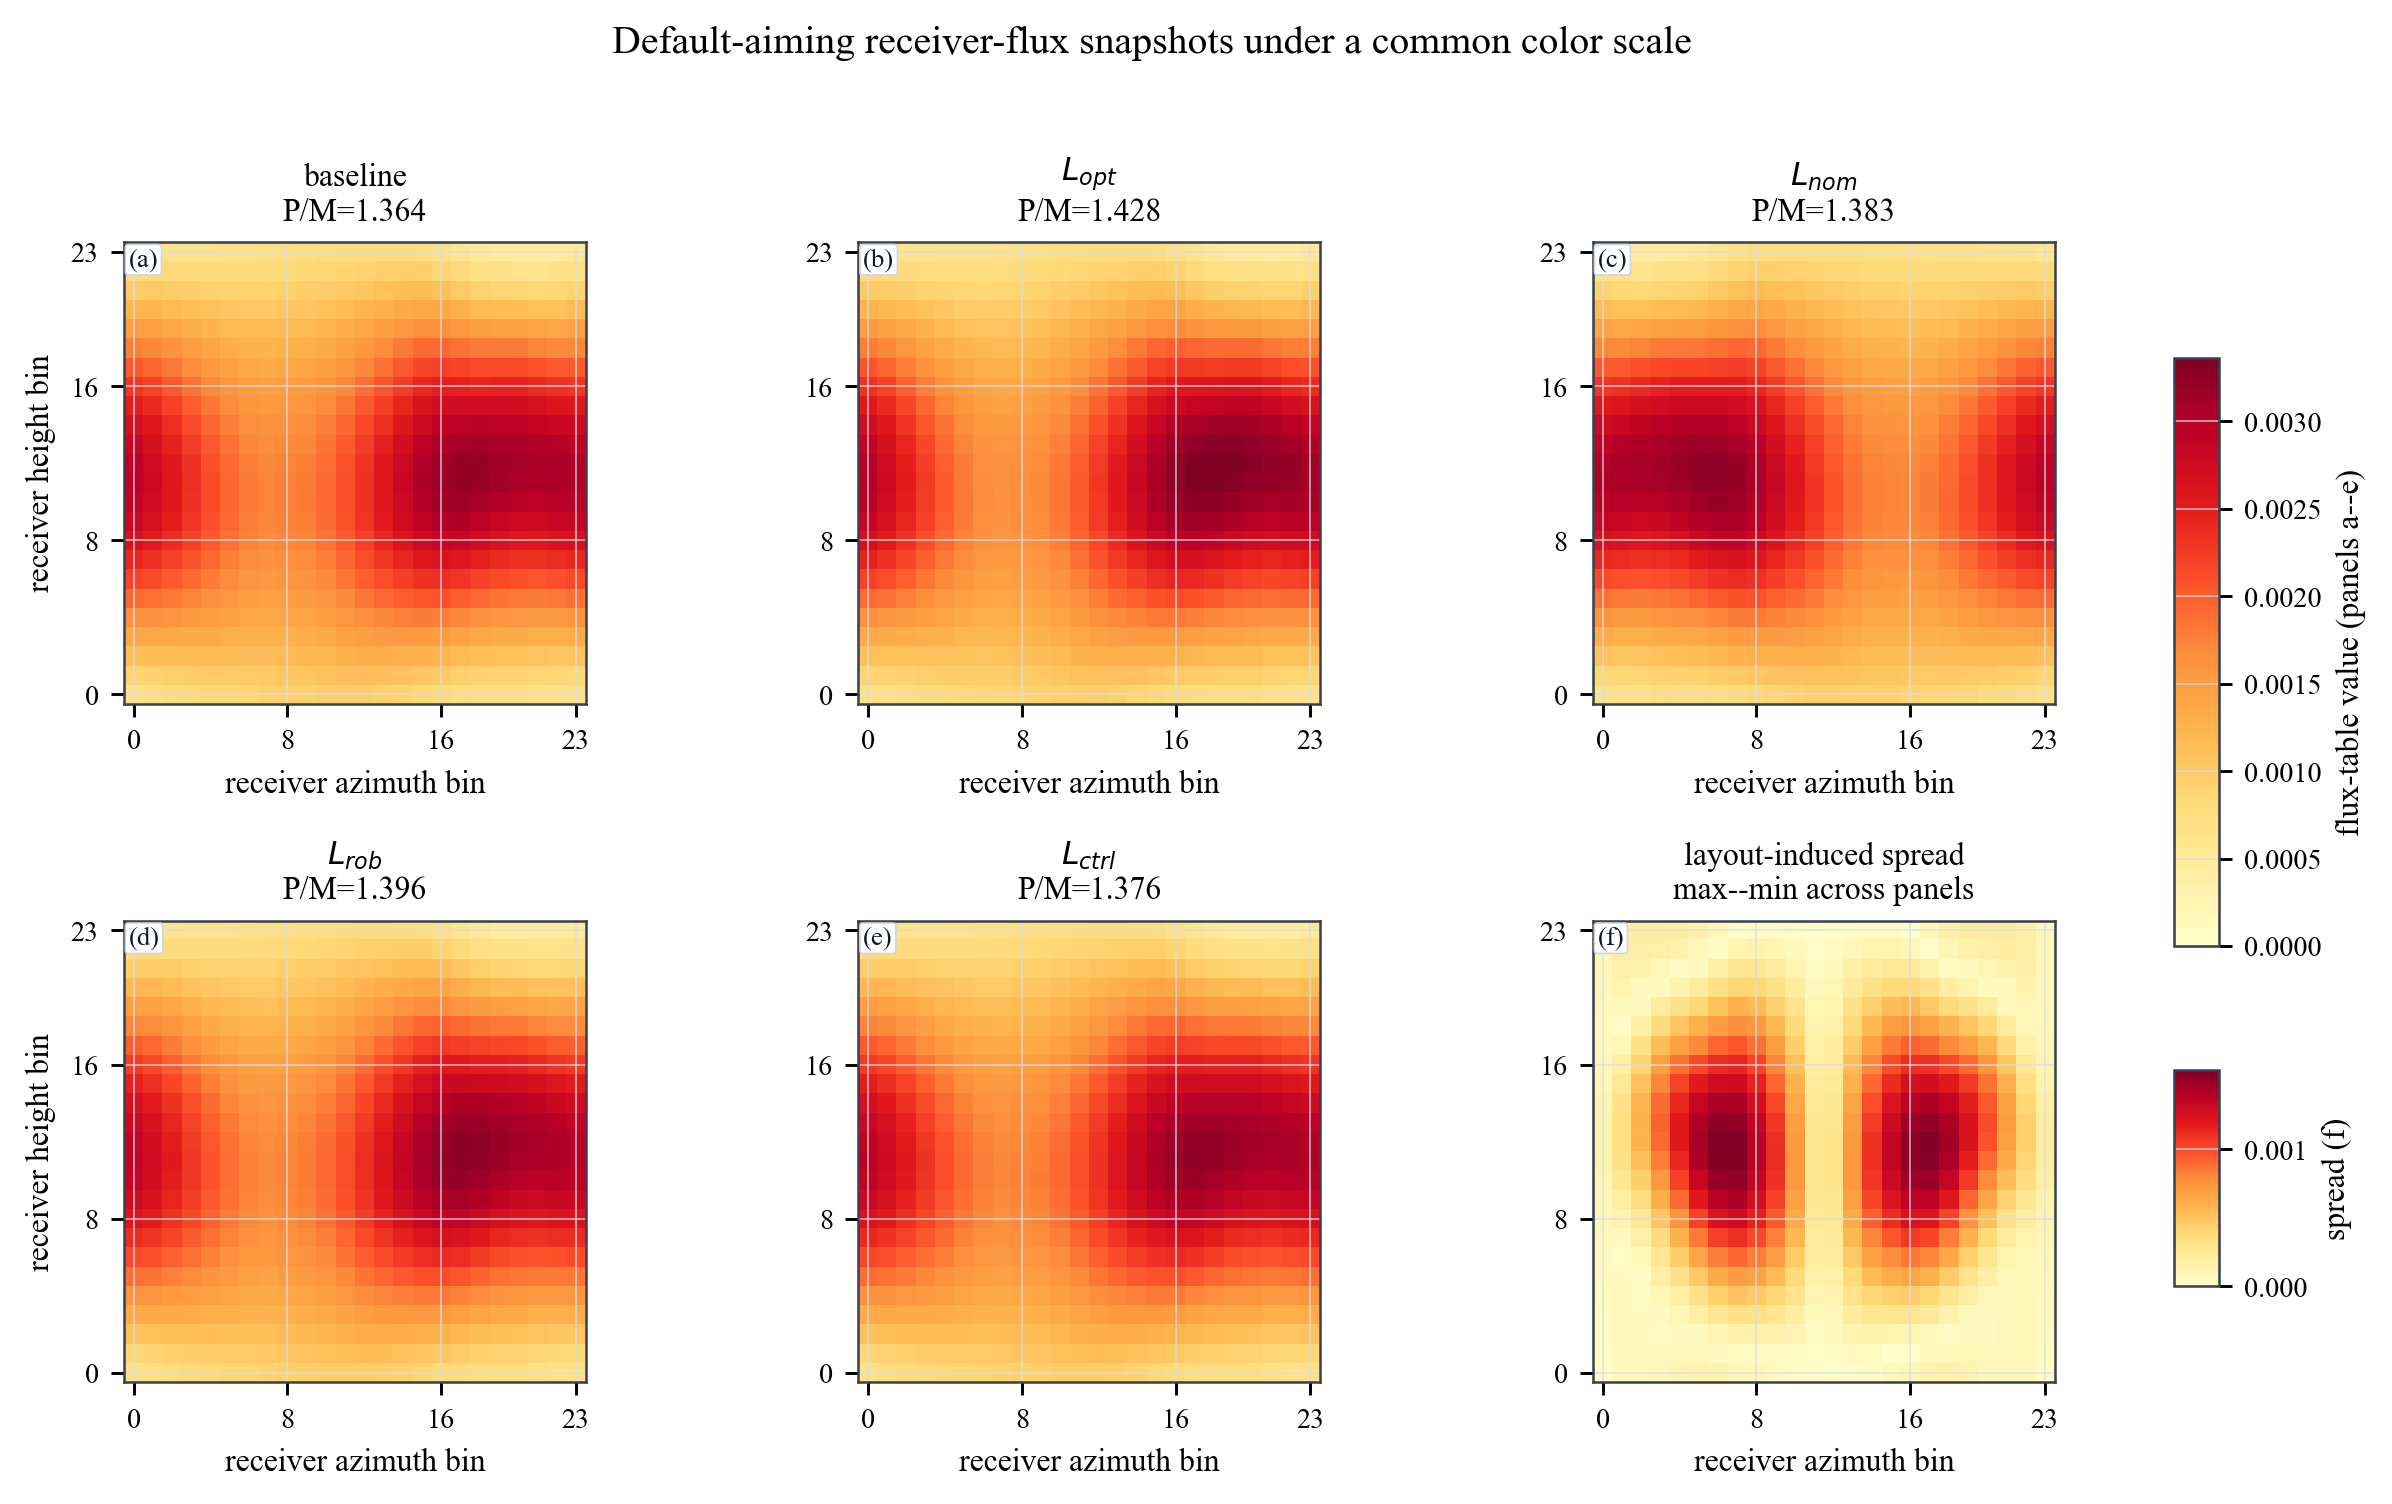
\includegraphics[width=0.92\textwidth]{figures/fig_journal_flux_peak_panel.png}
\caption{Default-aiming SolarPILOT receiver-flux snapshots for selected layouts under a common color scale. Panels (a)--(e) show the five layouts used in the high-resolution numerical check; panel (f) reports the cellwise layout-induced spread across those maps, making the sixth panel an audit summary rather than an unrelated extra candidate.}
\label{fig:fluxmaps}
\end{figure}

\subsection{Aiming-proxy queue}
The best initially searched staggered strategy for $L_{nom}$ reduces proxy peak-to-mean concentration by 6.22\% relative to the best searched baseline strategy while maintaining an intercept proxy of approximately 99.36\%. $L_{opt}$ is also important because it combines the strongest high-resolution SolarPILOT optical gain with a nominal 5.47\% aiming-proxy reduction. These nominal proxy results do not prove custom-aimpoint success. They define hypotheses for sensitivity testing and later optical-engine checking.

\begin{table}[t]
\centering
\caption{How the current representative candidates should be interpreted.}
\label{tab:candidate-meaning}
\small
\begin{tabular}{p{0.18\textwidth}p{0.29\textwidth}p{0.41\textwidth}}
\toprule
Candidate & Current evidence & Manuscript meaning \\
\midrule
$L_{opt}$ & Highest numerically checked optical gain but higher default flux concentration & Optical upper case; important as a stress test because proxy-aiming robustness is weak. \\
$L_{nom}$ & Best nominal aiming-proxy reduction with small positive default optical gain & Useful next-stage custom-aimpoint candidate, but not dominant under sensitivity. \\
$L_{ctrl}$ & Positive optical gain with the smallest high-resolution default-flux penalty among selected non-baseline layouts & Conservative default-flux control and robust sensitivity candidate. \\
$L_{rob}$ & Lowest screening flux-risk index and strongest median sensitivity improvement & Robust receiver-risk candidate, despite higher SolarPILOT default-flux penalty. \\
$L_0$ & Audited field reference & Required control for every percentage change. \\
\bottomrule
\end{tabular}
\end{table}

\begin{figure}[t]
\centering
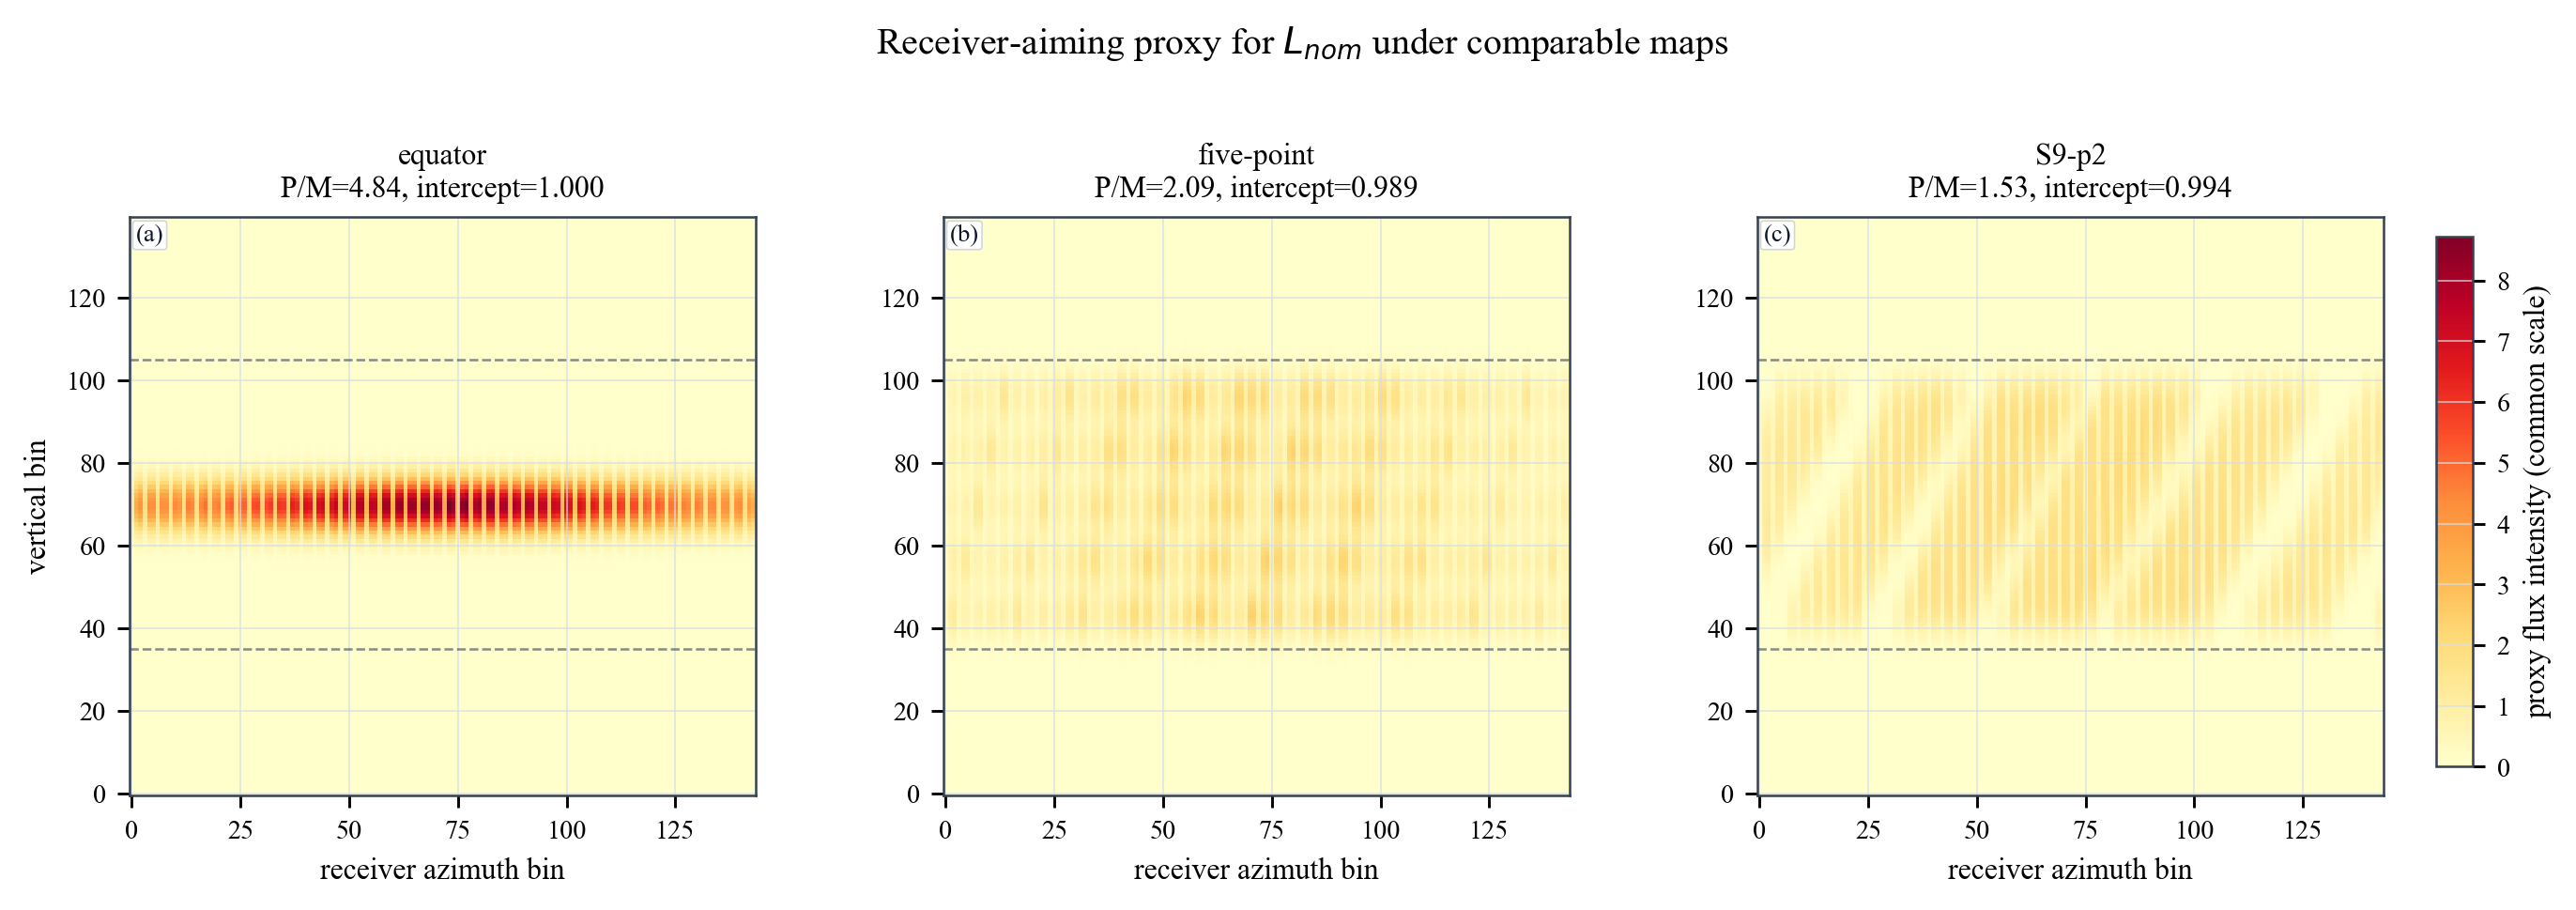
\includegraphics[width=0.90\textwidth]{figures/aiming_flux_deform_0893.png}
\caption{Receiver-aiming proxy maps for $L_{nom}$. The staggered strategy is a candidate generated by the proxy layer; reduced SolTrace results show that such proxy candidates still require direct checking before being treated as robust receiver-risk reductions.}
\label{fig:aimproxy}
\end{figure}

\subsection{Aiming-proxy sensitivity}
The nominal proxy ranking is not treated as sufficient evidence, because the proxy contains choices about sector grouping, annular grouping, azimuthal spot width, vertical spot width, and staggered phase. A deeper sensitivity sweep therefore perturbs these assumptions and re-optimizes the best proxy aiming strategy for each layout under 81 assumption combinations. Table~\ref{tab:aiming-sensitivity} and Fig.~\ref{fig:aiming-sensitivity} summarize the result.

The sensitivity result is not reduced to a single winner. $L_{rob}$ has the strongest median peak-to-mean reduction, improving 72\% of the tested assumptions with a median change of -1.94\% and negligible median intercept change. $L_{ctrl}$ also improves more often than it worsens, but with a smaller median change of -0.21\%. $L_{nom}$ remains useful because it was the nominal single-condition proxy leader and improves 64\% of assumptions, but its median reduction is only -0.32\%. In contrast, $L_{opt}$ improves only 32\% of assumptions and has a median increase of +0.61\% in proxy peak-to-mean concentration. This weakens any claim that the optical upper case is also an aiming-robust receiver-risk candidate.

The proxy layer also records a useful uncertainty cue. Improvements below roughly 1\% are not interpreted as robust reductions unless they are supported by the direct PySolTrace checks. This rule affects $L_{nom}$ and $L_{ctrl}$ in the proxy-sensitivity table: their median proxy changes are useful for queueing, but they are too small to serve as standalone evidence of receiver-risk improvement.

\begin{table}[t]
\centering
\caption{Aiming-proxy sensitivity across 81 grouping, spot-width, and staggered-phase assumptions. Negative peak-to-mean change indicates lower proxy concentration relative to the re-optimized baseline under the same condition.}
\label{tab:aiming-sensitivity}
\scriptsize
\begin{tabular*}{\textwidth}{@{\extracolsep{\fill}}lrrrr@{}}
\toprule
Layout & Lower frac. & Median $\Delta R_{aim}$ (\%) & P10/P90 $\Delta R_{aim}$ (\%) & Median $\Delta I$ (pct-pt) \\
\midrule
$L_{rob}$ & 0.72 & -1.94 & -5.32/+1.95 & +0.000 \\
$L_{nom}$ & 0.64 & -0.32 & -4.42/+1.31 & -0.008 \\
$L_{ctrl}$ & 0.63 & -0.21 & -1.06/+1.24 & -0.000 \\
$L_{opt}$ & 0.32 & +0.61 & -0.87/+2.86 & -0.001 \\
\bottomrule
\end{tabular*}
\end{table}

\begin{figure}[t]
\centering
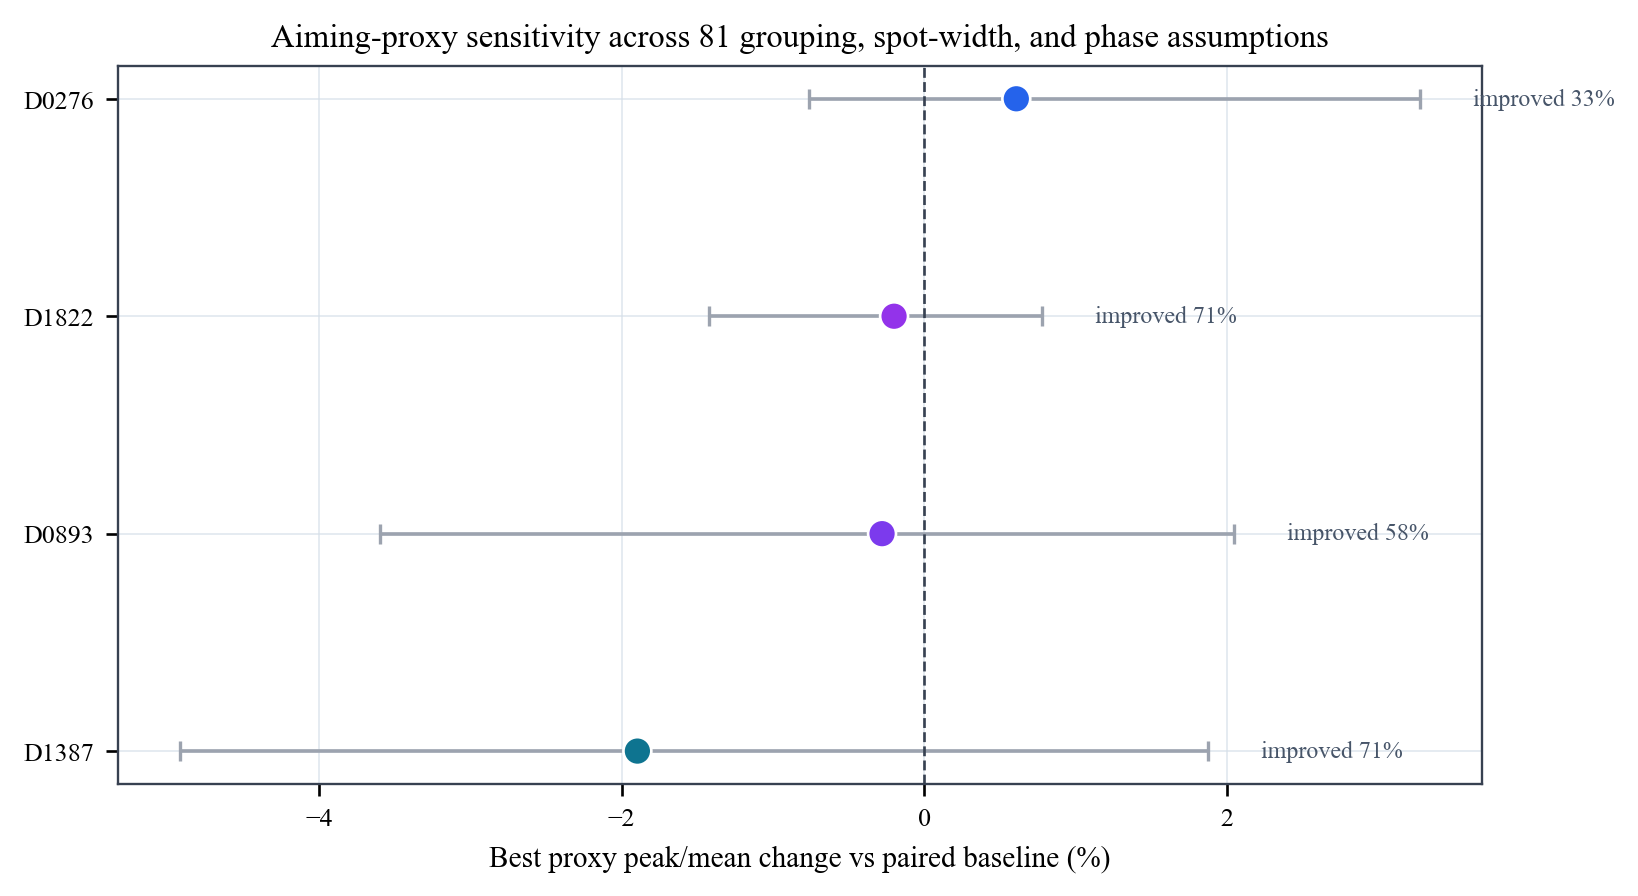
\includegraphics[width=0.80\textwidth]{figures/aiming_sensitivity_boxplot.png}
\caption{Sensitivity of best proxy aiming peak-to-mean change under alternative sector counts, annular counts, azimuthal spot widths, vertical spot widths, and staggered phases. The sensitivity sweep shifts the robust receiver-risk queue toward $L_{rob}$ and $L_{ctrl}$, while $L_{opt}$ remains mainly an optical upper case.}
\label{fig:aiming-sensitivity}
\end{figure}

\subsection{All-phase reduced SolTrace matrix with verified stage ordering}
The proxy results were followed by an enlarged reduced PySolTrace matrix to test whether candidate roles survive direct custom aimpoints. The matrix traces the heliostat reflector stage first and the receiver absorber stage second. This stage-order audit is not a minor implementation detail: with verified reflector-to-receiver ordering, receiver intercept ratios range from 0.639 to 0.748 across the 1,485 cases, so the receiver is no longer treated as if every requested ray were automatically absorbed. The all-phase test uses 6,000 stratified heliostats per layout, 60,000 requested first-stage ray hits per case, 18 flat receiver panels approximating the public cylindrical receiver, nine representative days, three daytime hours, and 11 aiming strategies: visible-equator, five-point, and all nine S9 staggered phases.

Table~\ref{tab:soltrace-corrected} separates two views of the all-phase results. The proxy-selected view asks whether the staggered phase selected by the screening proxy transfers to direct ray tracing over all 27 solar conditions. It transfers in a limited but useful way: the mean peak-to-active-mean concentration decreases for all four non-baseline layouts, but median changes are small and lower-peak fractions remain between 0.56 and 0.70. The best-direct view asks which tested layout--strategy row is best under the enlarged matrix. The strongest mean reduction is $L_{rob}$ with S9-p1 (-2.98\%), followed by $L_{nom}$ with S9-p2 (-2.78\%) and $L_{ctrl}$ with S9-p0 (-2.32\%). $L_{opt}$, the SolarPILOT optical upper case, remains the weakest direct receiver-risk candidate in this all-phase layer (-0.82\% mean change). The result is therefore a cross-layer diagnostic, not a universal optimization claim.

Because this matrix uses 60,000 requested first-stage ray hits per case, the peak metric is treated as a ranking diagnostic rather than a converged receiver-design quantity. The reported percentages should be read together with lower-peak fraction, median change, and the V9/V10 stability checks below. Layout--strategy differences smaller than the seed and sampling shifts are described as numerically indistinguishable, not as design improvements.

\begin{table}[H]
\centering
\caption{All-phase reduced PySolTrace matrix with verified reflector-to-receiver stage ordering. Negative values indicate lower peak-to-active-mean receiver concentration than the paired baseline under the same day, hour, and aiming strategy. The top block reports each layout's proxy-selected staggered strategy; the lower block reports the best direct strategy for each layout across all 27 solar conditions and 11 aiming strategies.}
\label{tab:soltrace-corrected}
\tiny
\begin{tabular*}{\textwidth}{@{\extracolsep{\fill}}lllrrrrr@{}}
\toprule
View & Layout & Strategy & Cases & Mean $\Delta R$ (\%) & Median $\Delta R$ (\%) & Lower frac. & Median $\Delta I$ (pct-pt) \\
\midrule
Proxy-selected & $L_{rob}$ & S9-p1 & 27 & -2.98 & -0.66 & 0.70 & -0.043 \\
Proxy-selected & $L_{nom}$ & S9-p2 & 27 & -2.78 & -0.36 & 0.56 & -0.117 \\
Proxy-selected & $L_{ctrl}$ & S9-p1 & 27 & -2.32 & -0.59 & 0.59 & +0.188 \\
Proxy-selected & $L_{opt}$ & S9-p0 & 27 & -0.82 & -0.40 & 0.67 & +1.357 \\
\midrule
Best direct & $L_{rob}$ & S9-p1 & 27 & -2.98 & -0.66 & 0.70 & -0.043 \\
Best direct & $L_{nom}$ & S9-p2 & 27 & -2.78 & -0.36 & 0.56 & -0.117 \\
Best direct & $L_{ctrl}$ & S9-p0 & 27 & -2.32 & -8.62 & 0.74 & +0.137 \\
Best direct & $L_{opt}$ & S9-p0 & 27 & -0.82 & -0.40 & 0.67 & +1.357 \\
\bottomrule
\end{tabular*}
\end{table}

Figure~\ref{fig:soltrace-corrected} is designed to make this diagnostic readable without forcing the reader to decode the full 1,485-row matrix. Panel (a) reports the mean, median, and P10--P90 spread of the best direct row for each layout, so the reader can see both the average benefit and its condition-level volatility. Panel (b) compares proxy-selected rows with the best direct rows, separating a useful screening signal from a final strategy choice. Panel (c) keeps the complete layout--strategy response surface, but marks only the best direct row (B) and the proxy-selected row (P) to avoid a table-like heatmap. The figure therefore carries the main message of the reduced ray-tracing layer: the candidate roles are informative, while the exact aiming phase remains a verification object.

\begin{figure}[H]
\centering
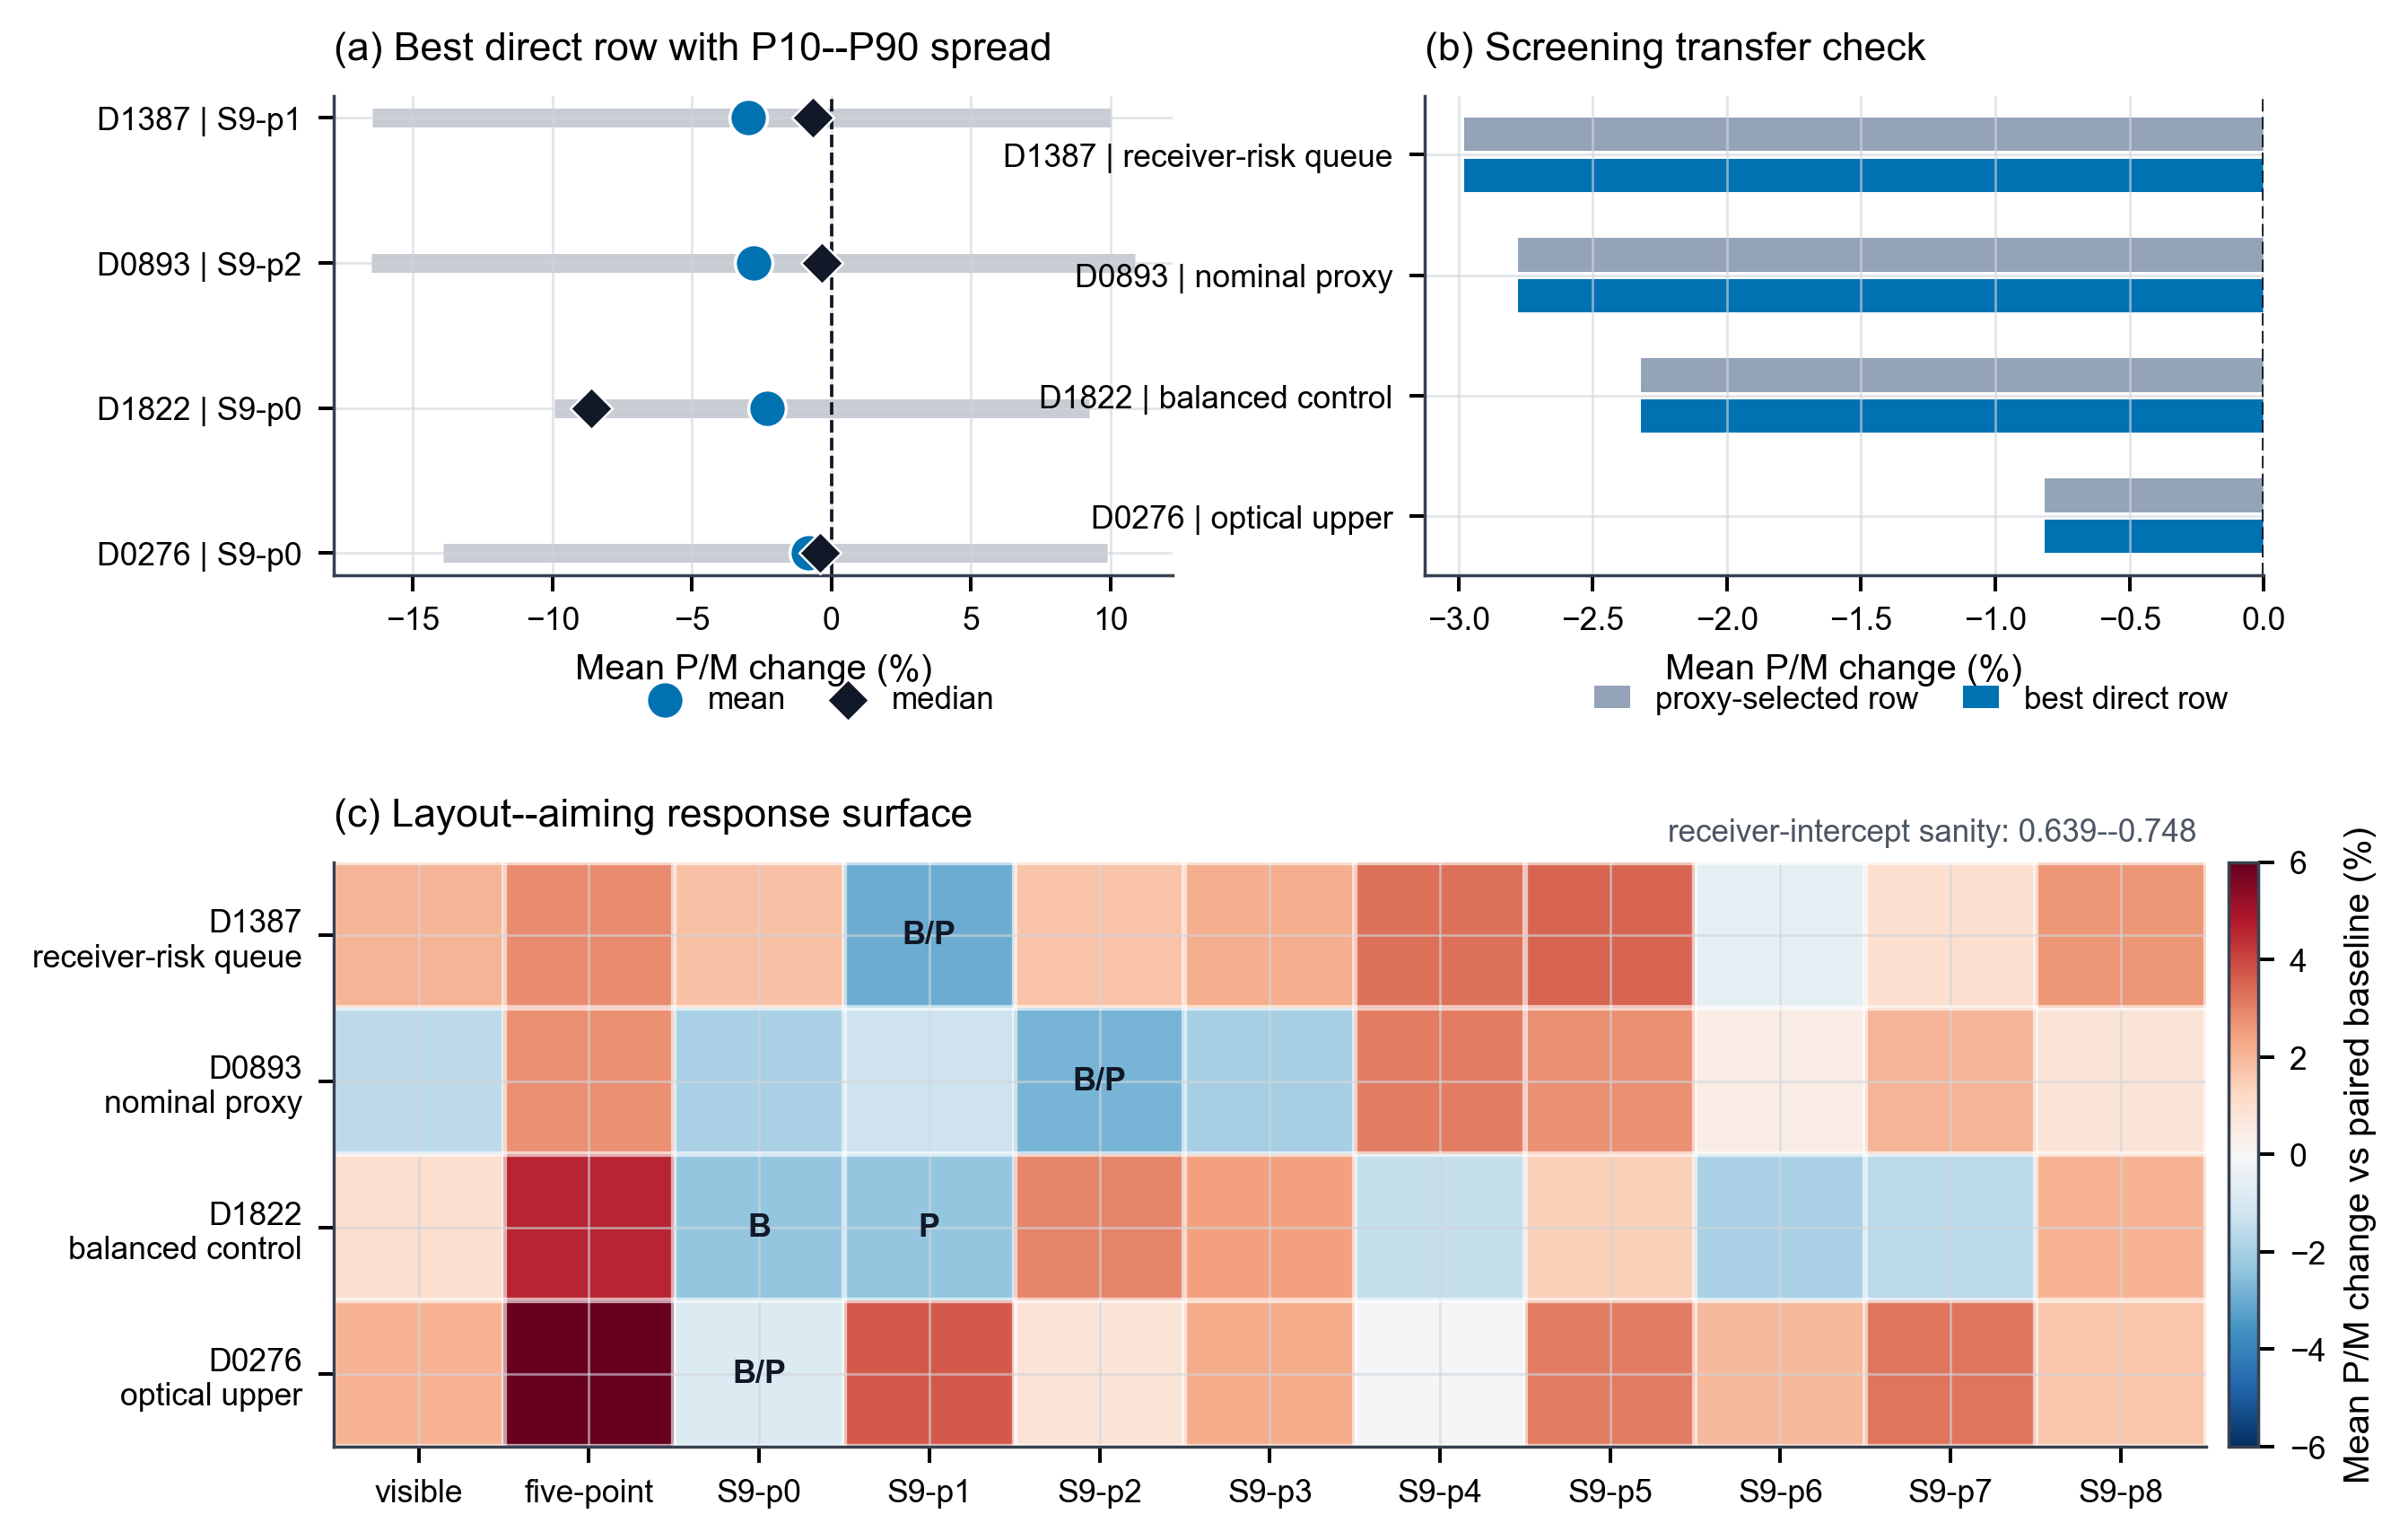
\includegraphics[width=0.92\textwidth]{figures/fig_soltrace_allphase_direct_panel.png}
\caption{All-phase reduced PySolTrace direct-aiming check. Panel (a) reports the best direct row for each layout with mean, median, and P10--P90 spread. Panel (b) compares proxy-selected aiming rows with the best direct rows. Panel (c) shows the complete layout--strategy response surface; blue cells indicate lower peak-to-active-mean receiver concentration than the paired baseline, red cells indicate higher concentration, B marks the best direct row, and P marks the proxy-selected row.}
\label{fig:soltrace-corrected}
\end{figure}

\subsection{Reduced direct-ray robustness consolidation}
The high-sample, independent-seed, and 240k-ray PySolTrace follow-up layers are retained in the supplementary package as audit tables rather than expanded in the journal body. Their purpose is narrow: they test whether the role-level queue suggested by the all-phase matrix survives changes in sampling density, receiver-panel discretization, stratified seed, and requested ray count. They do not create a new plant-optimal layout or a final annual custom-aimpoint schedule.

The consolidated result is intentionally cautious. The high-sample layer increases the sampled field from 6,000 to 9,000 heliostats per layout, increases the requested first-stage ray hits from 60,000 to 180,000 per case, and refines the receiver approximation from 18 panels to 24 panels with a 24 by 72 grid. The independent-seed replicate keeps the same layouts, strategies, and 27 solar conditions but redraws the stratified field sample. The V12 follow-up further raises the requested first-stage ray hits to 240,000 for the five verification-relevant strategies. Across these layers, the receiver-risk queue remains recognizable, but exact best aiming phases move. In particular, $L_{nom}$ is the only V12 best-direct row whose bootstrap mean confidence interval stays below zero (-3.41\%, 95\% CI [-6.48, -0.35]\%), while $L_{ctrl}$ has a higher lower-peak fraction but a confidence interval crossing zero. $L_{opt}$ remains mainly an optical stress case rather than a receiver-risk winner. These checks are why the manuscript reports role-level evidence and a direct-promotion queue rather than engineering superiority.

The full V9, V10, V11, and V12 tables, together with the source condition-level rows, are provided in the supplementary package and registered in the checksum manifest. This keeps the reproducibility evidence available to reviewers without making the main article read like a run log.

\iffalse

\subsection{High-sample reduced PySolTrace confirmation}
The high-sample confirmation run is used as a robustness check rather than as a new optimization claim. It keeps the same five layouts and the same 27 solar conditions, but increases the sampled field to 9,000 heliostats per layout, increases the requested first-stage ray hits to 180,000 per case, and refines the receiver approximation to 24 panels with a 24 by 72 grid. To control runtime, the confirmation matrix tests five verification-relevant strategies: visible-equator, five-point, and the S9 phases p0, p1, and p2. This produces 675 layout--strategy--condition cases. Receiver intercept ratios remain physically bounded, from 0.636 to 0.745, which is consistent with the stage-order sanity check in the all-phase layer.

Table~\ref{tab:v9-confirmation} gives the most important high-sample result. The V9 run preserves the role-level receiver-risk queue but not the exact V8 best strategy. None of the four non-baseline layouts keeps the same best row as in V8. For $L_{rob}$, the V8 best S9-p1 row becomes essentially neutral in V9 (+0.10\% mean change), while five-point aiming becomes the V9 best row (-3.41\%). For $L_{nom}$, the V8 S9-p2 row remains beneficial (-2.04\%) but is no longer the best row; S9-p1 gives -3.04\%. For $L_{ctrl}$, the V8 S9-p0 row becomes positive (+0.97\%), while five-point aiming gives -2.37\%. For $L_{opt}$, the V9 best row is weak (-0.40\%) and still much less compelling than the receiver-risk candidates. The confirmation layer therefore strengthens the benchmark interpretation: candidate roles are meaningful, but exact custom-aiming phases are sensitive to sampling and receiver discretization.

\begin{table}[t]
\centering
\caption{High-sample reduced PySolTrace confirmation. Negative values indicate lower peak-to-active-mean receiver concentration than the paired baseline. The confirmation run uses 9,000 sampled heliostats, 180,000 requested first-stage ray hits, five verification-relevant strategies, 27 solar conditions, 24 receiver panels, and a 24 by 72 receiver grid.}
\label{tab:v9-confirmation}
\scriptsize
\begin{tabular*}{\textwidth}{@{\extracolsep{\fill}}llrrrrrr@{}}
\toprule
Layout & V9 best strategy & V9 cases & V9 mean $\Delta R$ (\%) & V9 median $\Delta R$ (\%) & Lower frac. & Median $\Delta I$ (pct-pt) & V8 best same-row mean (\%) \\
\midrule
$L_{rob}$ & five-point & 27 & -3.41 & -5.65 & 0.56 & +0.024 & +0.10 \\
$L_{nom}$ & S9-p1 & 27 & -3.04 & -6.74 & 0.56 & -0.232 & -2.04 \\
$L_{ctrl}$ & five-point & 27 & -2.37 & -0.28 & 0.56 & +0.003 & +0.97 \\
$L_{opt}$ & S9-p1 & 27 & -0.40 & -0.67 & 0.67 & +1.169 & +1.78 \\
\bottomrule
\end{tabular*}
\end{table}

\begin{figure}[t]
\centering
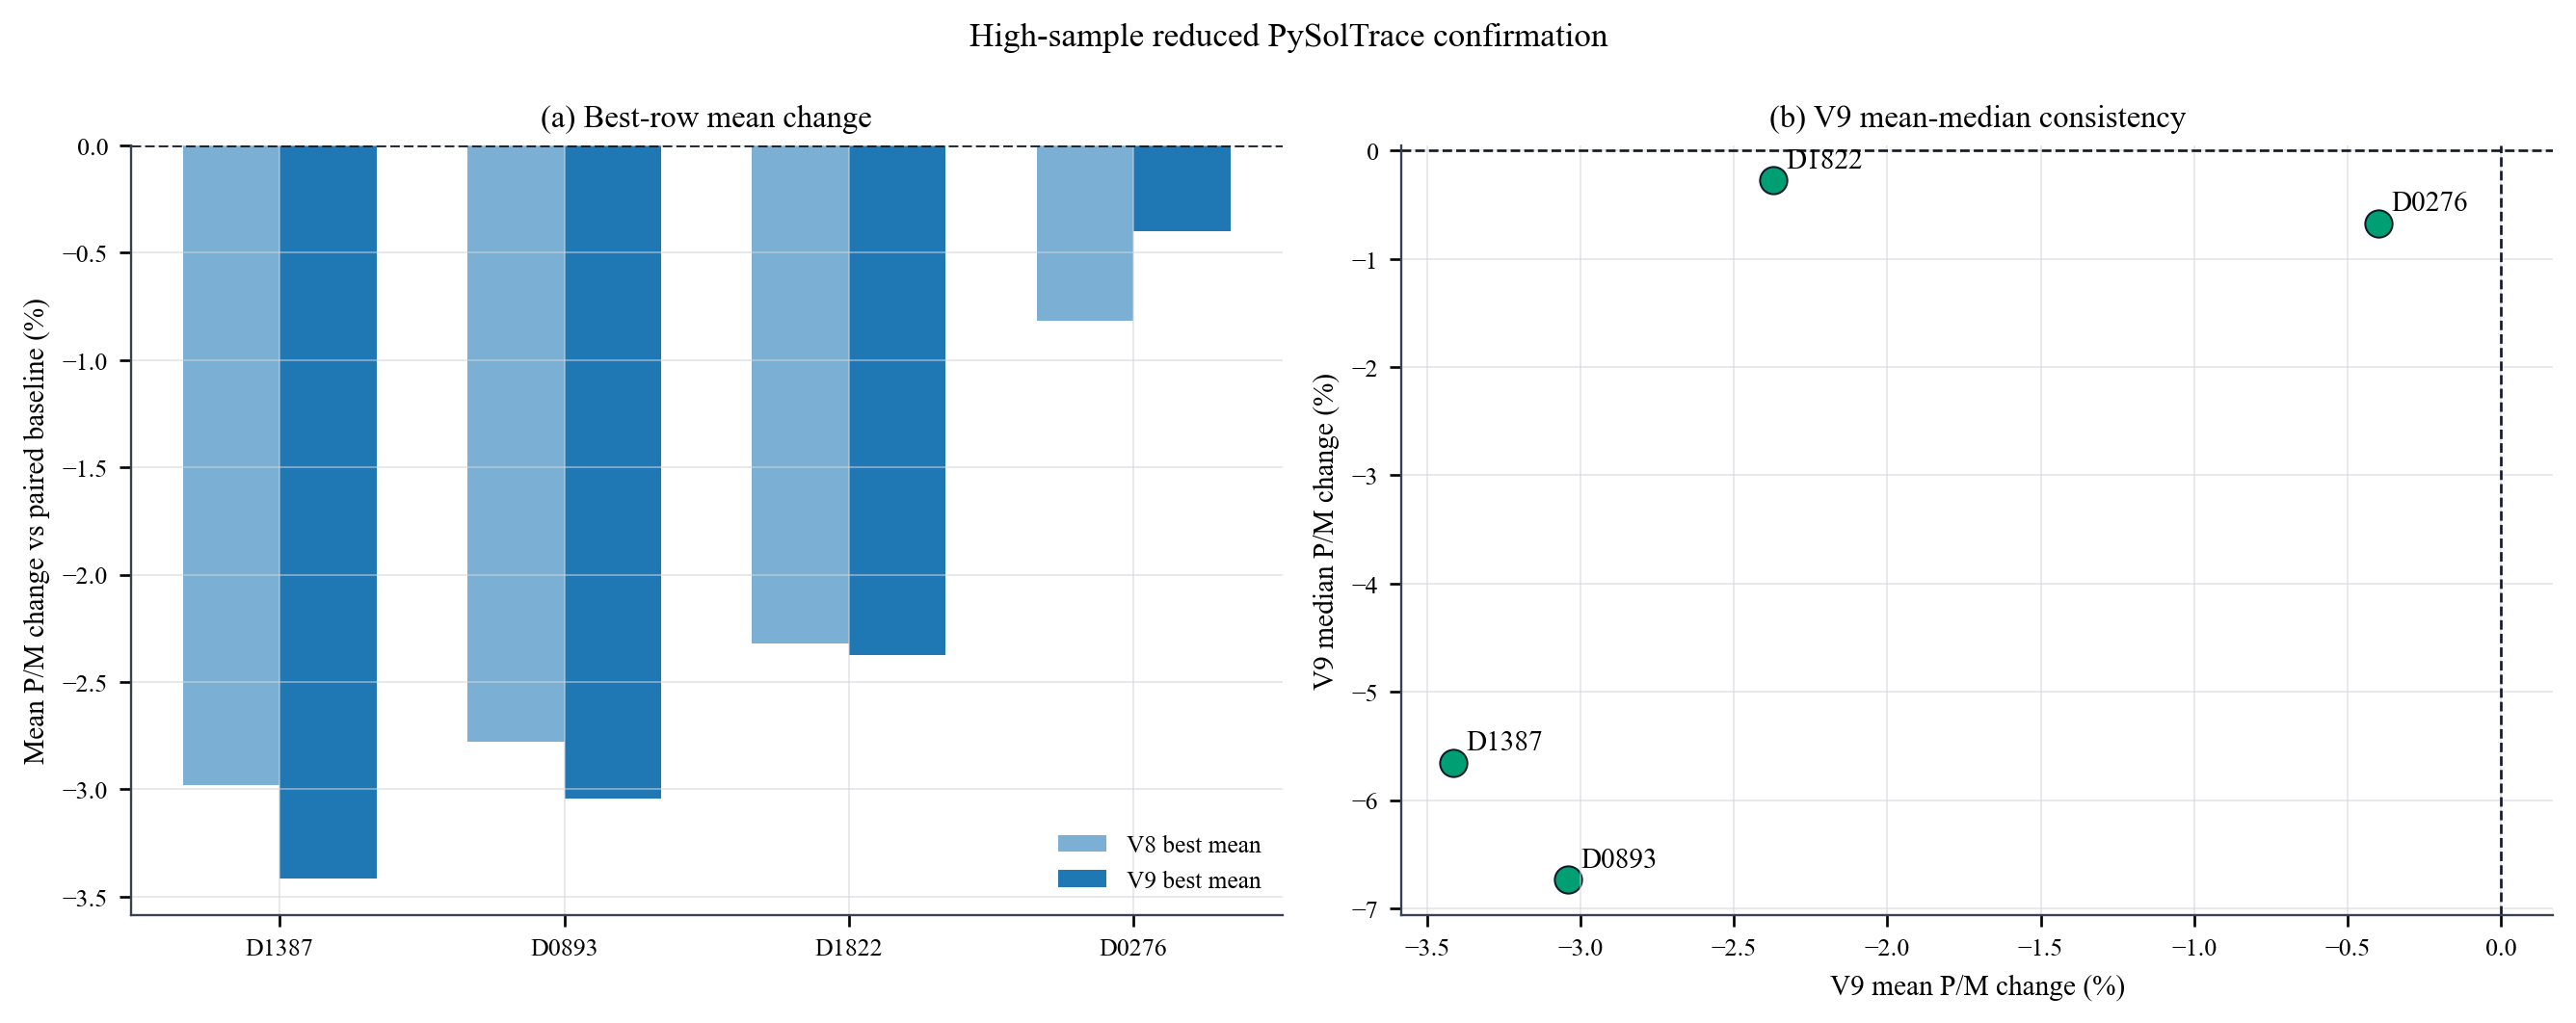
\includegraphics[width=0.92\textwidth]{figures/fig_v9_highsample_confirmation.png}
\caption{High-sample reduced PySolTrace confirmation. Panel (a) compares the best-row mean peak-to-active-mean change from the all-phase V8 matrix and the higher-sample V9 matrix. Panel (b) shows that the V9 mean and median changes do not always tell the same story, reinforcing the need to treat this layer as reduced direct checking rather than final plant certification.}
\label{fig:v9-confirmation}
\end{figure}

\subsection{Independent-seed V10 stability audit}
The V9 confirmation layer already showed that exact best direct-aiming rows can move when the sampled field and receiver discretization are changed. The V10 replicate tests the same five layouts, the same 27 solar conditions, the same five verification-relevant strategies, the same 9,000 sampled heliostats per layout, the same 180,000 requested first-stage ray hits per case, and the same 24-panel, 24 by 72 receiver grid, but with an independent stratified seed. The purpose is not to claim a new layout winner. The purpose is to check whether the receiver-risk candidate queue survives a fresh sampling pass.

Table~\ref{tab:v10-stability} shows the key result. The candidate roles remain recognizable: $L_{rob}$ is still the strongest receiver-risk layout, $L_{ctrl}$ remains competitive, $L_{nom}$ stays in the middle of the queue, and $L_{opt}$ remains the weakest of the four non-baseline layouts. But the exact best strategies change again. In V10, $L_{rob}$ is best under S9-p1, $L_{ctrl}$ is best under S9-p0, and both $L_{nom}$ and $L_{opt}$ prefer five-point aiming. None of the four non-baseline layouts keeps the same best strategy as in V9. That result is not a failure of the benchmark. It is the benchmark working as intended: the candidate queue is more stable than the exact reduced-check phase.

\begin{table}[t]
\centering
\caption{Independent-seed V10 stability audit. Negative values indicate lower peak-to-active-mean receiver concentration than the paired baseline. V10 uses the same layouts, strategies, and solar conditions as V9, but a fresh stratified sample and the same 24-panel, 24 by 72 receiver grid.}
\label{tab:v10-stability}
\scriptsize
\begin{tabular*}{\textwidth}{@{\extracolsep{\fill}}llrrrrrr@{}}
\toprule
Layout & V9 best strategy & V9 best mean \% & V10 best strategy & V10 best mean \% & V10 same-row mean \% & Same best? & Mean shift \% \\
\midrule
$L_{rob}$ & five-point & -3.41 & S9-p1 & -2.69 & -0.65 & No & +0.72 \\
$L_{ctrl}$ & five-point & -2.37 & S9-p0 & -2.48 & -2.32 & No & -0.10 \\
$L_{nom}$ & S9-p1 & -3.04 & five-point & -2.33 & -2.33 & No & +0.71 \\
$L_{opt}$ & S9-p1 & -0.40 & five-point & -0.31 & -0.31 & No & +0.09 \\
\bottomrule
\end{tabular*}
\end{table}

\begin{figure}[t]
\centering
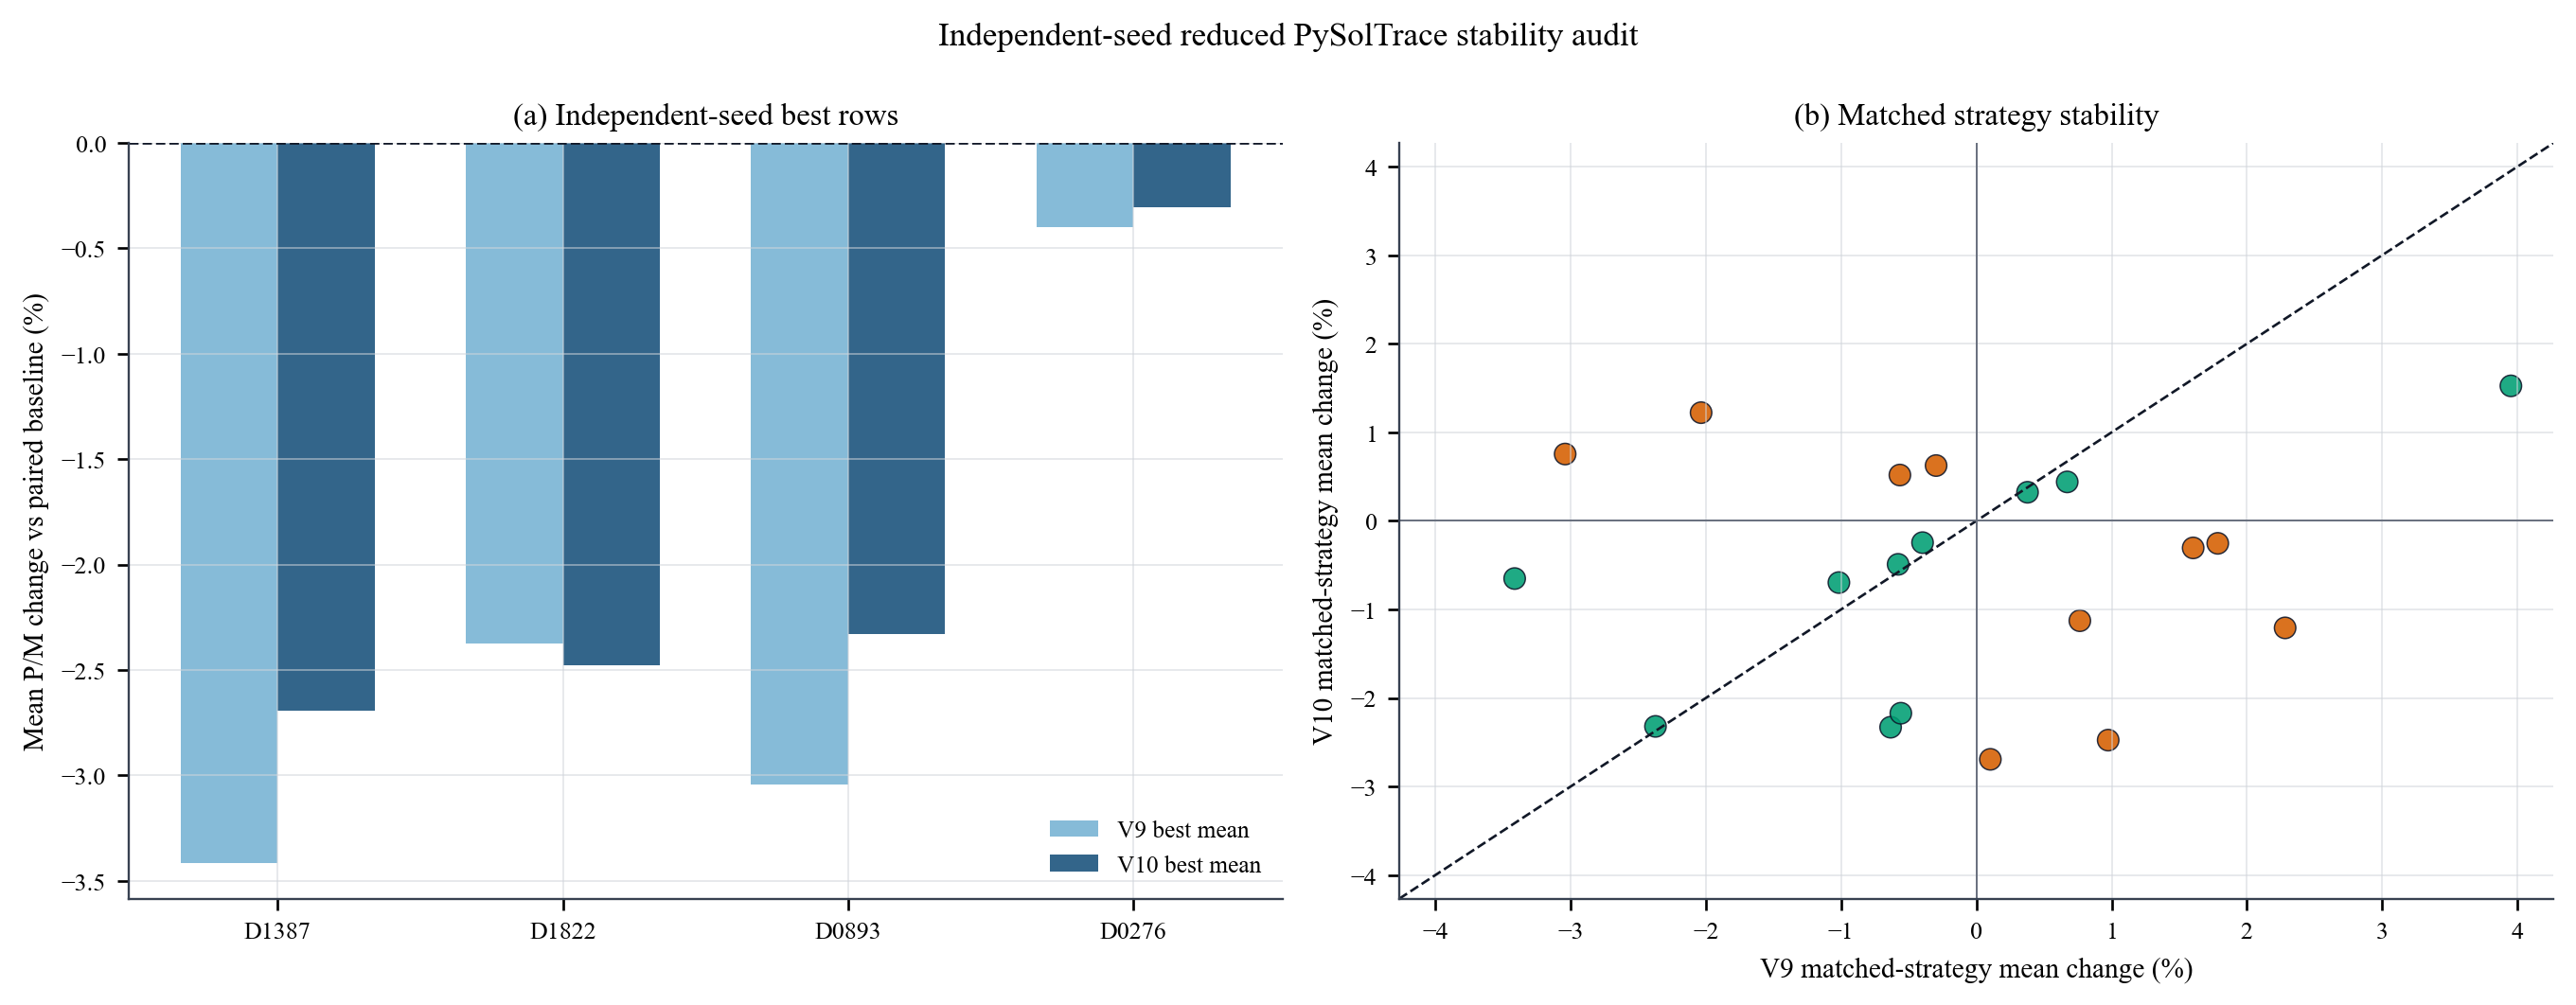
\includegraphics[width=0.92\textwidth]{figures/fig_v10_seed_replicate_stability.png}
\caption{Independent-seed V10 stability audit. Panel (a) compares the best-row mean peak-to-active-mean change from V9 and V10. Panel (b) shows the matched-strategy mean changes for the shared layout--strategy pairs. The queue remains recognizable, but the exact best direct-aiming phase changes under a fresh stratified sample.}
\label{fig:v10-stability}
\end{figure}

\subsection{Convergence and uncertainty audit}
The three reduced PySolTrace layers are finally consolidated as a convergence and uncertainty audit. This audit is not a new optimization pass. It asks a narrow reproducibility question: which part of the reduced direct-check result is stable enough to support the manuscript, and which part should remain a future verification target?

Table~\ref{tab:v11-convergence} and Fig.~\ref{fig:v11-convergence} give the answer. Across V8, V9, and V10, all four non-baseline layouts keep negative best-row mean peak-to-active-mean changes, but the strength of that signal differs sharply. The receiver-risk candidates remain ahead of the optical-upper layout: $L_{rob}$ spans -2.69\% to -3.41\%, $L_{nom}$ spans -2.33\% to -3.04\%, and $L_{ctrl}$ spans -2.32\% to -2.48\%, while $L_{opt}$ stays weak, from -0.31\% to -0.82\%. The best-row range is also modest for the role-level queue, especially for $L_{ctrl}$ (0.16 percentage points), but the exact aiming strategy is not stable. The matched-strategy sign-consistency fraction is only 0.45 from V8 to V9 and 0.50 from V9 to V10; the median absolute matched-row mean shift is 2.62 and 1.79 percentage points, respectively. These values are larger than several of the claimed peak-to-mean improvements, so the paper reports candidate roles rather than a final aiming prescription.

\begin{table}[t]
\centering
\caption{Reduced PySolTrace convergence and uncertainty audit. The table consolidates the all-phase V8 matrix, the high-sample V9 confirmation, and the independent-seed V10 replicate. Negative best-row mean values indicate lower peak-to-active-mean receiver concentration than the paired baseline under the same audit layer.}
\label{tab:v11-convergence}
\scriptsize
\begin{tabular*}{\textwidth}{@{\extracolsep{\fill}}llrrrrr@{}}
\toprule
Layout & Role & V8 best mean \% & V9 best mean \% & V10 best mean \% & Best-row range pct-pt & Stable best sign? \\
\midrule
$L_{rob}$ & Receiver-risk & -2.98 & -3.41 & -2.69 & 0.72 & Yes \\
$L_{nom}$ & Nominal-proxy & -2.78 & -3.04 & -2.33 & 0.71 & Yes \\
$L_{ctrl}$ & Default-flux-control & -2.32 & -2.37 & -2.48 & 0.16 & Yes \\
$L_{opt}$ & Optical-upper & -0.82 & -0.40 & -0.31 & 0.51 & Yes, but weak \\
\bottomrule
\end{tabular*}
\end{table}

\begin{figure}[t]
\centering
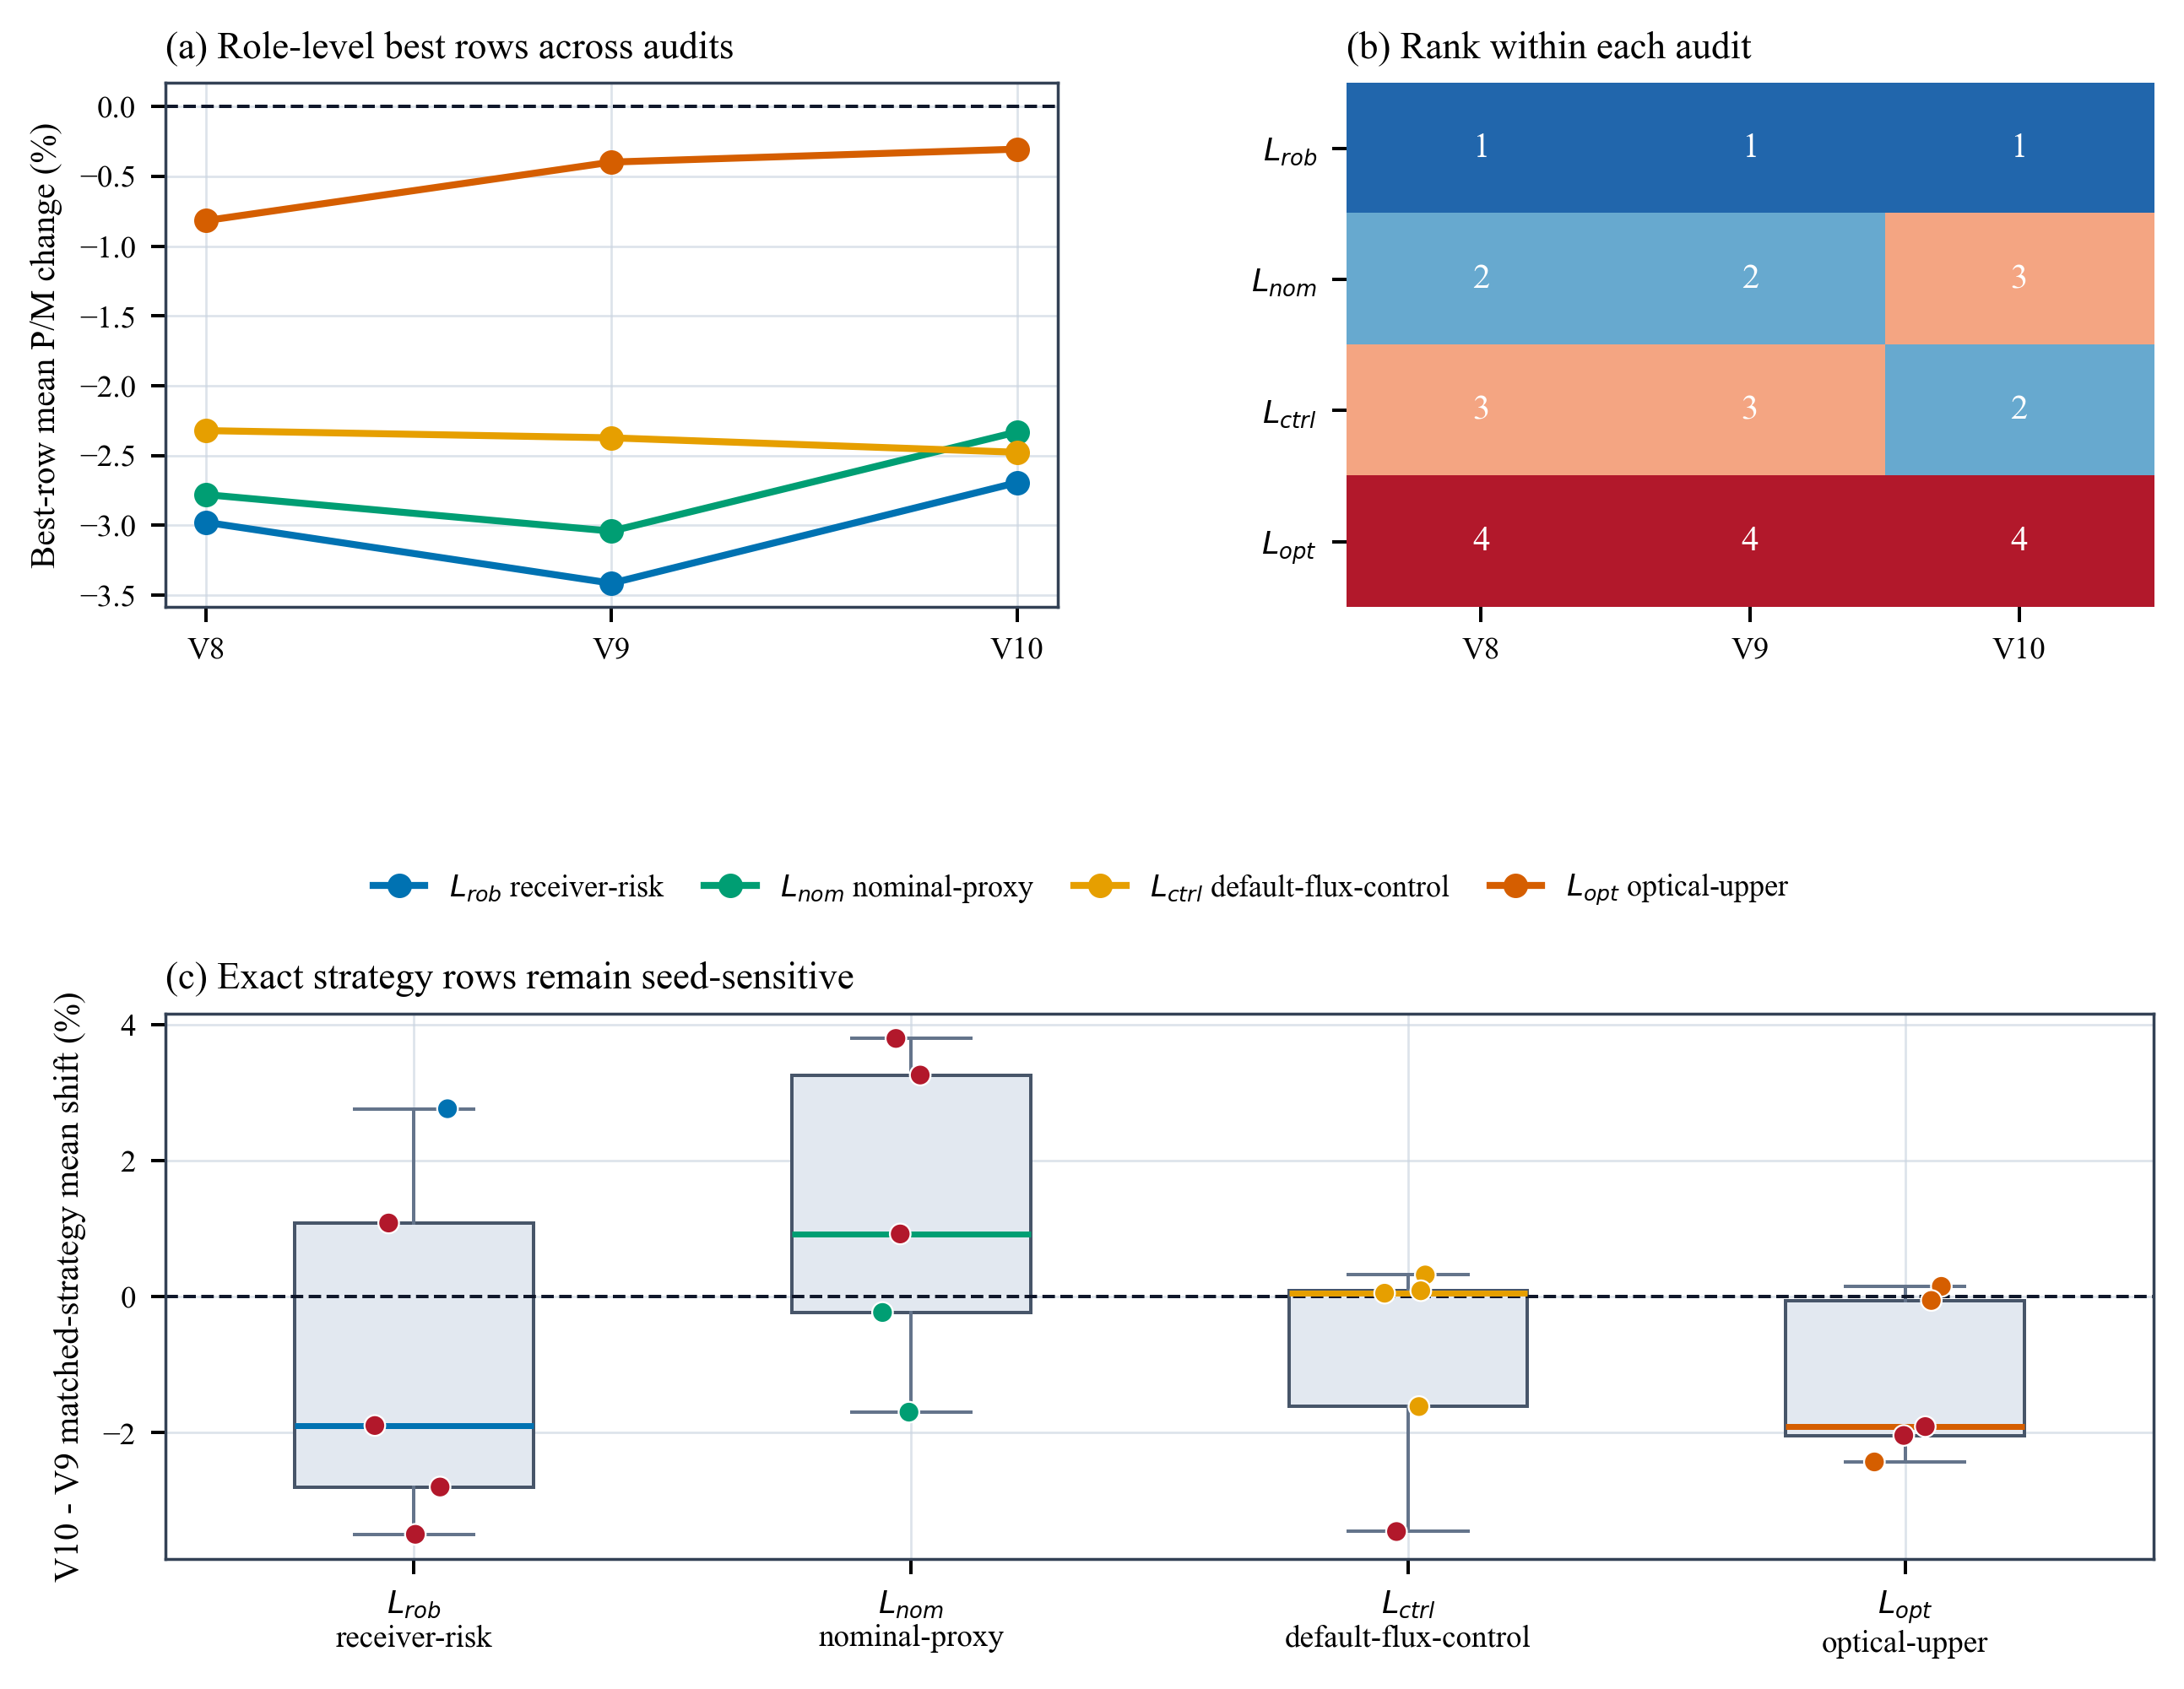
\includegraphics[width=0.95\textwidth]{figures/fig_v11_soltrace_convergence_audit.png}
\caption{Reduced PySolTrace convergence and uncertainty audit. Panel (a) tracks each layout role's best-row mean peak-to-active-mean change across V8, V9, and V10. Panel (b) ranks the four non-baseline roles within each audit layer. Panel (c) shows the V10--V9 matched-strategy shifts; red points indicate rows whose mean-change sign flips under the independent seed. The figure supports a stable receiver-risk queue but not a final single aiming phase.}
\label{fig:v11-convergence}
\end{figure}

\subsection{V12 240k-ray follow-up audit}
After the V11 consolidation, a higher-ray reduced audit was run to check whether the receiver-risk queue remains useful when the high-sample matrix is enlarged from 180,000 to 240,000 requested first-stage ray hits per case. The V12 follow-up uses the same five layouts, 27 solar conditions, 9,000 sampled heliostats per layout, 24 receiver panels, and 24 by 72 receiver grid as the V9/V10 scale, but tests five verification-relevant strategies: visible-equator, five-point, and S9 phases p0--p2. It produces 675 layout--strategy--condition rows and keeps receiver intercept ratios within the same physically bounded range, approximately 0.636--0.744.

The useful result is narrower than a new optimum. $L_{nom}$ becomes the strongest V12 direct-check candidate under S9-p1, with a mean peak-to-active-mean change of -3.41\%, a median change of -5.48\%, and a lower-peak fraction of 0.56. $L_{ctrl}$ is also supported: its proxy-selected S9-p1 row gives a mean change of -2.13\%, a median change of -4.86\%, and the highest lower-peak fraction among the proxy-selected rows, 0.74. $L_{opt}$ has only a weak best V12 reduction (-0.39\% mean under S9-p2), and its proxy-selected S9-p0 row is unfavourable (+3.40\% mean). $L_{rob}$ is nearly neutral in this follow-up (-0.04\% mean under S9-p1). The V12 layer is therefore written into the paper as a strengthening of the role-level screening interpretation, especially for $L_{nom}$ and $L_{ctrl}$, not as evidence that every previously named receiver-risk candidate improves under all higher-ray checks.

\begin{table}[t]
\centering
\caption{V12 240k-ray reduced PySolTrace follow-up. Negative values indicate lower peak-to-active-mean receiver concentration than the paired baseline under the same day, hour, and aiming strategy. The table reports the best direct row for each non-baseline layout at the V12 scale.}
\label{tab:v12-followup}
\scriptsize
\begin{tabular*}{\textwidth}{@{\extracolsep{\fill}}llrrrr@{}}
\toprule
Layout & V12 best strategy & Cases & Mean $\Delta R$ (\%) & Median $\Delta R$ (\%) & Lower frac. \\
\midrule
$L_{nom}$ & S9-p1 & 27 & -3.41 & -5.48 & 0.56 \\
$L_{ctrl}$ & S9-p1 & 27 & -2.13 & -4.86 & 0.74 \\
$L_{opt}$ & S9-p2 & 27 & -0.39 & -0.45 & 0.70 \\
$L_{rob}$ & S9-p1 & 27 & -0.04 & -0.25 & 0.63 \\
\bottomrule
\end{tabular*}
\end{table}

To address uncertainty explicitly, the V12 condition-level rows were also bootstrapped with replacement within each layout--strategy row. The bootstrap uses the 27 representative solar conditions as the resampling unit and 10,000 replicates. Table~\ref{tab:v12-bootstrap} reports the best direct V12 row for each non-baseline layout. Only $L_{nom}$ has a best-row mean confidence interval that remains below zero, although its lower-peak fraction is modest. $L_{ctrl}$ has a stronger lower-peak fraction, but its bootstrap interval crosses zero. $L_{opt}$ and $L_{rob}$ should therefore remain bounded evidence cases rather than headline improvements. This is a useful negative result: the larger ray count strengthens the case for a receiver-risk screening queue, but it does not justify a final custom-aiming optimum.

\begin{table}[t]
\centering
\caption{Bootstrap confidence audit for the V12 240k-ray reduced PySolTrace layer. Confidence intervals resample the 27 representative solar conditions within each layout--strategy row. Negative values indicate lower peak-to-active-mean concentration than the paired baseline under the same strategy and condition.}
\label{tab:v12-bootstrap}
\scriptsize
\begin{tabular*}{\textwidth}{@{\extracolsep{\fill}}lllrrr@{}}
\toprule
Layout & Role & V12 best strategy & Mean $\Delta R$ (\%) & 95\% bootstrap CI (\%) & Lower frac. \\
\midrule
$L_{nom}$ & nominal-proxy & S9-p1 & -3.41 & [-6.48, -0.35] & 0.56 \\
$L_{ctrl}$ & default-flux-control & S9-p1 & -2.13 & [-5.46, +1.46] & 0.74 \\
$L_{opt}$ & optical-upper & S9-p2 & -0.39 & [-3.70, +3.13] & 0.70 \\
$L_{rob}$ & receiver-risk & S9-p1 & -0.04 & [-2.96, +3.27] & 0.63 \\
\bottomrule
\end{tabular*}
\end{table}
\FloatBarrier

\fi

\subsection{Formal paired-statistics audit}
The reduced direct matrices were finally recast as paired condition-level experiments, because mean changes alone can make weak rows look stronger than they are. For each selected layout--strategy row, the paired sample is the 27-condition vector of peak-to-active-mean changes against the same baseline, day, hour, and aiming strategy. The audit reports bootstrap 95\% confidence intervals for the mean, Hodges--Lehmann median shifts, one-sided sign tests, one-sided Wilcoxon signed-rank tests, and a deliberately conservative $\pm$1 percentage-point practical-indistinguishability band. The full table is included in \path{supplementary_data/formal_paired_statistics/}; Table~\ref{tab:formal-paired} reports the rows that matter most for the manuscript claim.

\begin{table}[t]
\centering
\caption{Formal paired-statistics summary for the key reduced direct rows. Confidence intervals bootstrap the 27 paired solar-condition deltas. The Wilcoxon test uses the one-sided alternative that the candidate has lower peak-to-active-mean concentration than the paired baseline.}
\label{tab:formal-paired}
\scriptsize
\begin{tabular*}{\textwidth}{@{\extracolsep{\fill}}llllrrrr@{}}
\toprule
Matrix & Candidate & View & Strategy & Mean $\Delta R$ (\%) & 95\% CI (\%) & HL shift (\%) & Wilcoxon $p$ \\
\midrule
Baseline-control direct & $L_{rob}$ & best direct & S9-p2 & -3.61 & [-6.17, -0.97] & -4.49 & 0.035 \\
Joint direct promotion & $J_{flux}$ & proxy/best direct & S9-p5 & -4.06 & [-6.99, -0.93] & -4.64 & 0.006 \\
V12 240k direct & $L_{nom}$ & best direct & S9-p1 & -3.41 & [-6.48, -0.35] & -2.77 & 0.089 \\
Joint direct promotion & $J_{bal}$ & proxy/best direct & S9-p2 & -1.98 & [-6.59, +2.98] & -4.45 & 0.053 \\
Joint direct promotion & $J_{gain}$ & proxy selected & S9-p3 & +2.58 & [-1.54, +6.67] & +1.88 & 0.907 \\
\bottomrule
\end{tabular*}
\end{table}

The statistical audit does not create a new positive headline. It narrows the claim in a useful way. $L_{rob}$ in the baseline-control direct matrix, $J_{flux}$ in the joint direct matrix, and $L_{nom}$ in the V12 240k-ray follow-up have bootstrap mean intervals below zero. $J_{bal}$ remains directional and close to a one-sided Wilcoxon threshold, but its confidence interval crosses zero. The proxy-selected $J_{gain}$ row is adverse. No row has its entire 95\% confidence interval below the -1\% practical threshold, so the manuscript should continue to use the phrase ``screening queue'' rather than ``engineering superiority'' or ``final prescription.''

\begin{figure}[t]
\centering
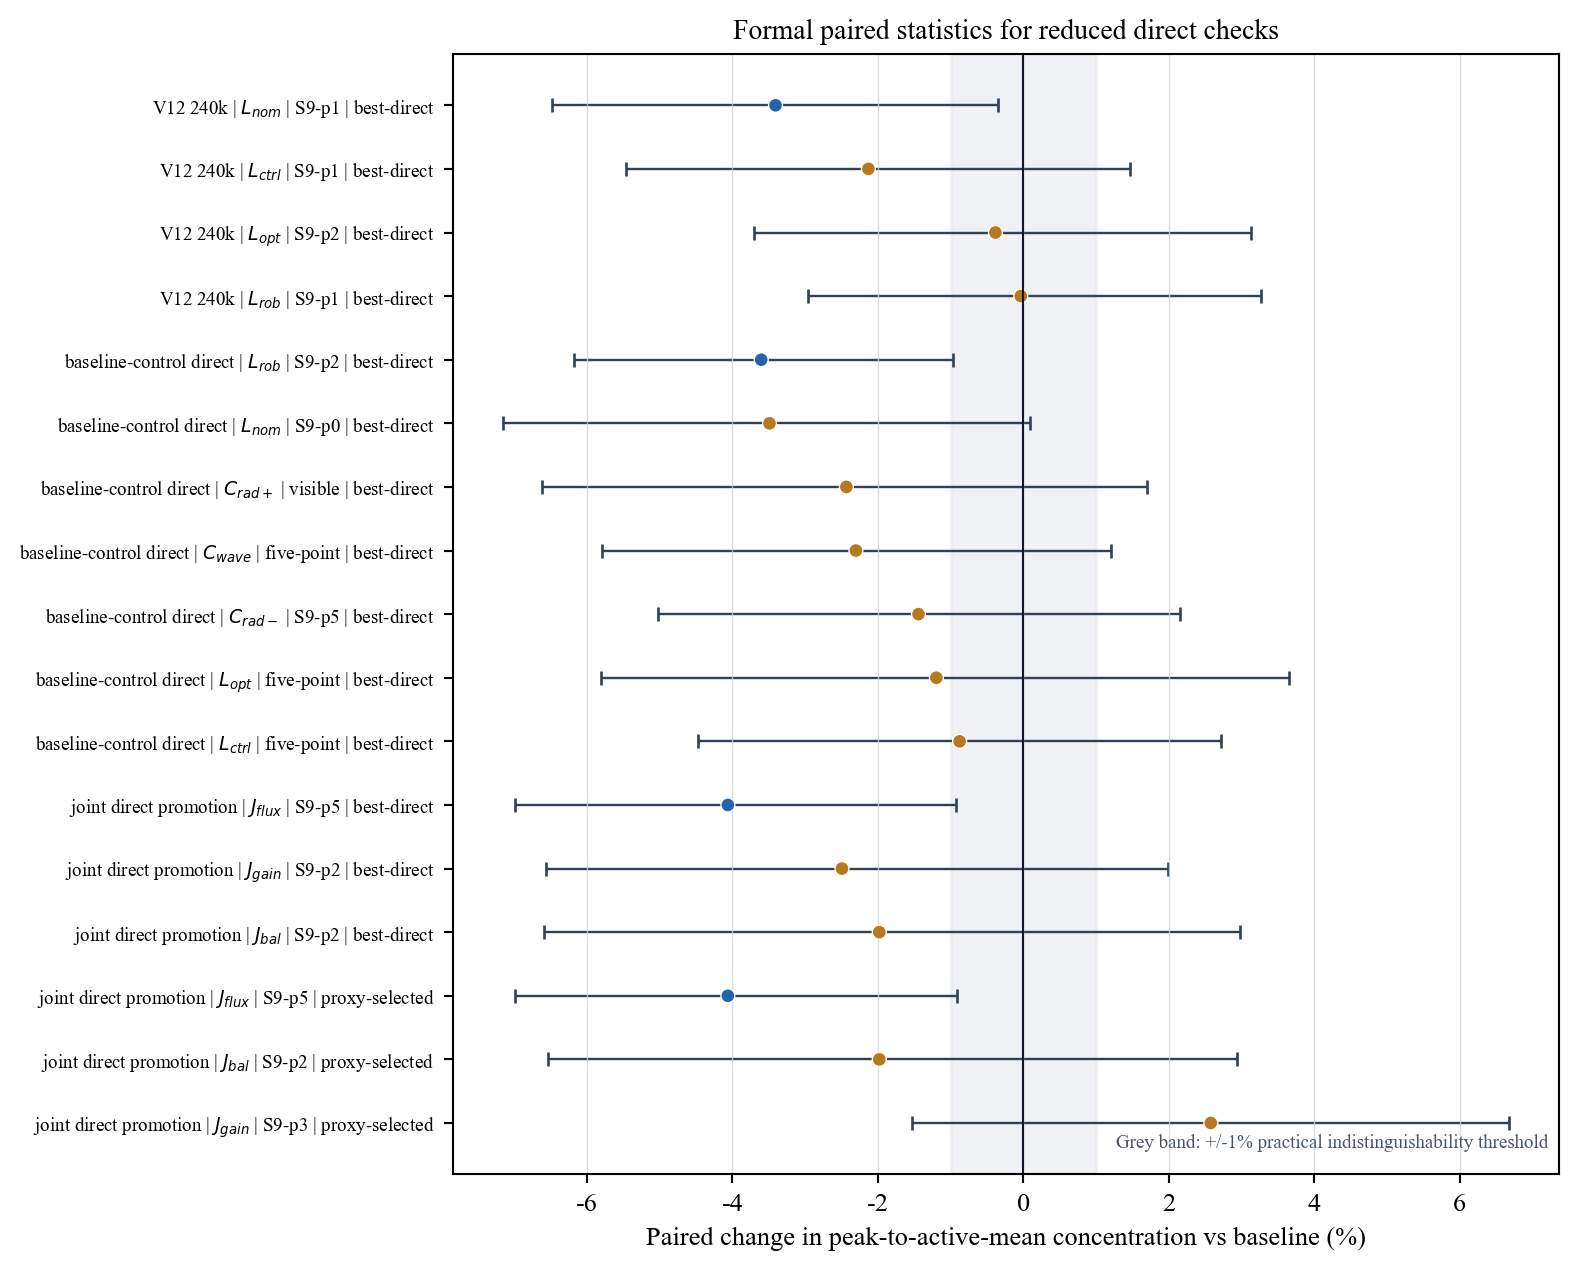
\includegraphics[width=0.92\textwidth]{figures/fig_formal_paired_statistics.png}
\caption{Formal paired-statistics audit for selected reduced direct rows. Points show mean paired changes in peak-to-active-mean receiver concentration, whiskers show 95\% bootstrap confidence intervals over the 27 representative solar conditions, and the grey band marks the $\pm$1\% practical-indistinguishability threshold.}
\label{fig:formal-paired}
\end{figure}
\FloatBarrier

\section{Discussion}
\subsection{Why the full-field layout is credible}
The current field shape is consistent with the logic of large surround solar tower fields. It preserves plant scale, keeps field coverage continuous, and avoids the collapse produced by mirror deletion. Because access roads, foundations, blocked land parcels, heliostat calibration, and survey-grade terrain are not represented, the layout set is best interpreted as a computational benchmark for layout and receiver-flux method development rather than as an industrial redesign.

\subsection{Why the result is more than a module}
The contribution is a benchmark workflow rather than a layout preview. It connects plant audit, full-field deformation, feasibility filtering, geometry-explainability auditing, proxy screening, SolarPILOT numerical checking, relative AFD-style hotspot-area auditing, baseline-control testing, strong-baseline pressure testing, joint layout--aiming screening, direct promotion auditing, and formal paired statistics. This chain is useful because many layout studies optimize one scalar and then present a final field. Here, the workflow makes the trade-off visible and leaves a reproducible queue for higher-fidelity checking. In practical terms, $L_{opt}$ defines an optical upper case and its receiver-flux cost; $L_{nom}$ tests whether a nominal proxy leader transfers to direct tracing; and $L_{rob}$ and $L_{ctrl}$ test whether receiver-risk candidates remain informative when the sampling and receiver grid change. The geometry audit explains how these rows move: the largest selected p95 displacement is 107.5 m for $L_{opt}$, while several strong-baseline receiver-pressure rows stay below 46 m. The simple controls test whether those signals are merely radial expansion, compaction, or wave effects. The same-anchor strong-baseline pressure test then asks a harder question: whether pattern-free-, slider-like-, terrain-aware-, and hybrid-deformation approximations can explain the queue. They can explain part of it, especially through the hybrid and slider-like rows, which is why the manuscript avoids single-method superiority language. The joint run then tests whether layout deformation and aiming can be selected together rather than in separated modules. Its direct promotion audit is the most useful new result: $J_{flux}$ survives as a direct-supported receiver-boundary candidate, while $J_{bal}$ and $J_{gain}$ show why proxy-selected phases must pass a direct optical-engine gate. The formal paired-statistics audit is the final gate in the current package: it supports $J_{flux}$, $L_{rob}$, and the V12 $L_{nom}$ row as the clearest receiver-risk candidates, but it also confirms that no row should be written as final engineering superiority. The lack of a single final winner follows from the numerical evidence.

\subsection{Frontier fit}
The topic remains current, but the novelty threshold has increased. A study that only perturbs heliostat coordinates is unlikely to be sufficient because recent work already includes deformable petal layouts, uneven-terrain field tools, collision-analysis-based layouts, reinforcement-learning aiming, closed-loop flux control, neural surrogates, and differentiable ray tracing. The same-anchor strong-baseline pressure test is therefore important: it shows that hybrid and pattern-free approximation families can produce competitive local signals, so the manuscript should not be read as a standalone layout-optimization winner. The present contribution is narrower and more testable: it combines a public 100 MW plant anchor with full-field preservation, terrain audit, receiver-flux reporting, baseline pressure testing, and a reproducible screening queue that advanced aiming methods can reuse.

\subsection{Practical value}
The immediate practical value is upstream and computational rather than direct retrofit. Existing foundations, roads, wiring, calibration, and land agreements make physical relocation unrealistic for an operating field. The benchmark helps researchers test whether layout-level changes, receiver aiming, and optical verification methods agree on the same candidate. It also gives future optimization methods a more informative target than one final coordinate file: the geometry-explainability table states how far each candidate moves, the annual proxy states whether an optical signal survives a public weather year, and the direct-promotion rows state which receiver-risk hypotheses deserve more expensive checking. It can therefore inform new-field preliminary design, repowering studies, and algorithm comparisons without implying that the operating Dunhuang field should be physically rearranged.

\subsection{Negative results as evidence}
The flux penalty in the optical winner is central to the result. It demonstrates that the screening workflow is not tuned only to produce favorable optical-efficiency outcomes. The proxy sensitivity sweep adds a second negative result: the optical upper case $L_{opt}$ is not robustly favoured by the aiming proxy. The same-condition controls add a third boundary: simple radial expansion and radial-wave controls can reduce direct peak-to-active-mean concentration under some strategies, so the paper cannot attribute every receiver-risk signal to TS-FPDA. The all-phase reduced SolTrace matrix with verified stage ordering adds the first direct check for the TS-FPDA queue: all non-baseline candidates can reduce mean peak-to-active-mean concentration under at least one directly traced row, but the reductions are modest, condition-dependent, and not aligned with the SolarPILOT optical ranking. The baseline-control direct audit then shows that $L_{rob}$ is the only tested best-direct row with a bootstrap interval below zero, while $L_{nom}$ is close and the simple controls remain meaningful but uncertain. The V9/V10/V11 audit sharpens this point. It preserves the receiver-risk queue around $L_{rob}$, $L_{nom}$, and $L_{ctrl}$, but it also shows that exact strategy rows can change sign under higher sampling or an independent seed. The V12 follow-up further supports $L_{nom}$ as a useful next-stage candidate, while weakening any blanket claim that $L_{rob}$ or the optical upper case is consistently safer under enlarged reduced tracing. The joint direct audit adds a fourth boundary: integrated layout--aiming search can generate a stronger receiver-boundary candidate, but proxy-selected phases do not always transfer to direct tracing. The formal paired-statistics layer then turns these observations into an explicit evidence grade: $J_{flux}$, $L_{rob}$, and V12 $L_{nom}$ have intervals below zero, $J_{bal}$ and $L_{ctrl}$ are directional, and proxy-selected $J_{gain}$ is adverse. The verification question is therefore not whether one layout and one aiming phase are universally superior, but whether each candidate role remains useful under the verification layer being used.

\subsection{Remaining verification need}
The current evidence supports a reproducible benchmark and workflow claim, but not certification of a final plant redesign. The reduced PySolTrace layers provide direct custom-aimpoint evidence for selected layouts and representative solar conditions, yet they remain sampled audits with faceted receiver approximations rather than a full-field annual campaign. The AFD-style audit, receiver-bin and flux-day reruns, geometry-explainability audit, baseline controls, strong-baseline pressure test, annual-proxy gates, and formal paired statistics each remove a narrower reviewer concern; none of them turns the package into a receiver thermal-safety certificate or a bankable yield study.

The next verification layer should therefore be a statistically enlarged or full-field CoPylot/SolarPILOT, SolTrace, or Solstice study using matched solar conditions, aimpoint definitions, receiver grids, canting/focus assumptions, and normalization. The queue supplied by this manuscript is designed for that step: it keeps the optical upper case, nominal proxy leader, receiver-risk representatives, simple controls, strongest same-anchor pressure rows, and joint layout--aiming candidates in one auditable set. The reduced direct matrices also show why the next step should re-optimize or re-check aimpoint phases rather than freezing a single proxy-selected phase. This is the intended use of the package: a transparent promotion queue for higher-fidelity verification, not a finished prescription for the operating field.

\subsection{Domain of validity}
Table~\ref{tab:domain-validity} states the domain of validity used when interpreting the results. This table is intentionally conservative. It prevents the paper from sounding like an operating-plant redesign while preserving the part that is still useful to the research community: a transparent large-field case for testing layout generation, aiming strategies, receiver-flux metrics, and verification pipelines.

\begin{table}[t]
\centering
\caption{Domain of validity and claim boundary for the benchmark.}
\label{tab:domain-validity}
\small
\begin{tabular}{p{0.26\textwidth}p{0.32\textwidth}p{0.32\textwidth}}
\toprule
Question & Supported interpretation & Not supported by the current evidence \\
\midrule
Layout realism & Full-field, ellipse-like surround candidates near the public Dunhuang coordinate envelope & Official as-built survey or civil construction layout \\
Optimization claim & Candidate queue and trade-off benchmark under common assumptions & Globally optimal heliostat field or final plant redesign \\
Receiver-flux claim & Relative peak-to-active-mean screening under default SolarPILOT and reduced PySolTrace direct checks & Certified absolute receiver heat-flux safety or tube-temperature compliance \\
Terrain claim & Reproducible SRTM90m public-terrain screening & Survey-grade grading, drainage, foundation, or road-access design \\
Weather and annual claim & Public-weather relative comparison, uniform DNI scaling, fast annual optical proxy, and public design-generation sanity check & Bankable annual yield, dispatch model, or plant-grade TMY validation \\
Aiming claim & Candidate roles for future custom-aimpoint verification; exact phases are not stable enough to prescribe & Final annual custom-aimpoint schedule \\
Economic claim & No LCOE or retrofit economics claim; cost score is a triage indicator only & Commercial repowering or retrofit recommendation \\
\bottomrule
\end{tabular}
\end{table}

\subsection{Limitations}
The limitations are material. The available coordinate pool contains 11,915 non-origin heliostats rather than the reported 11,935. SRTM90m terrain is public and reproducible but not survey-grade. NASA POWER weather is reproducible but not the plant's corrected TMY; the multi-year gate checks sign and rank stability over public weather years, not measured operation. The fast annual proxy is an interpolation of SolarPILOT default-aiming optical-efficiency tables over public weather years and is used only as an annualization and plant-scale sanity bridge; the interpolation-robustness gate tests numerical mapping choices for that proxy, not measured annual performance. The annual proxy is not a dispatch simulation, bankable annual-yield estimate, or full-field custom-aimpoint annual ray trace. PySAM/SolarPILOT checks imported x/y positions under default aiming but not custom staggered aimpoints through the bridge used here. The AFD-style hotspot-area audit is relative to numerical baseline thresholds and is not an allowable-flux-density or tube-temperature model. The 36 by 36 flux-resolution and 12-flux-day sampling checks reduce default-flux numerical-discretization concern, but they do not certify receiver thermal safety. The reduced PySolTrace matrices, including the baseline-control direct and leave-one-day-out audits, check direct aimpoint logic only on stratified samples, faceted receiver approximations, and selected solar conditions. The same-anchor strong baselines are literature-inspired approximation families rather than complete reproductions of named external optimizers, so they strengthen the pressure test but do not settle a field-wide optimizer ranking. Proxy cost score is not sufficient for economic superiority claims.
\FloatBarrier

\section{Declaration of Generative-AI and AI-Assisted Technologies}
During the preparation of this work, the authors used ChatGPT and other AI-assisted writing tools to support literature organization, language polishing, figure-style iteration, and revision-risk checklist drafting. After using these tools, the authors reviewed and edited the manuscript, verified the scientific content, numerical results, citations, figures, and final claims, and take full responsibility for the content of the article.

\section{Conclusions}
This manuscript reconstructs the Dunhuang heliostat study as a plant-anchored layout--aiming benchmark. The full-field surround/ellipse-like candidates are engineering-plausible because they preserve the available 11,915-heliostat coordinate pool, avoid mirror-deletion collapse, and remain within conservative geometry bounds. The geometry-explainability audit confirms that the representative rows are local count-preserving redistributions rather than new plant concepts: the largest selected p95 movement scale is 107.5 m for $L_{opt}$, while the receiver-pressure strong-baseline rows remain below 46 m and retain stable spacing and sector coverage.

The central checked result is a trade-off. Small full-field geometric deformations can improve default SolarPILOT optical efficiency, but the optical upper case also increases receiver-flux concentration and the relative AFD-style active p99 hotspot-area proxy. A fast annual proxy keeps the optical ranking over public weather years and places the baseline proxy on the same order as the public 351.6 GWh design-generation reference, but it does not create a bankable annual-yield claim. The same-condition controls, direct baseline-control audit, and same-anchor strong-baseline pressure test show that simple and literature-inspired local deformations must remain in the comparison set. TS-FPDA is therefore useful as a conservative candidate-generation component inside the benchmark, not as a field-optimal layout method.

The joint layout--aiming layer is the main system-level extension. It searches layout deformation and receiver-aiming choices together, then uses SolarPILOT default-aiming checks, reduced PySolTrace direct promotion, and paired statistics to decide which hypotheses survive. The reduced direct promotion audit supports $J_{flux}$ as a receiver-boundary candidate, keeps $J_{bal}$ as a directional balance candidate, and downgrades $J_{gain}$ to a strategy-sensitivity case. The formal paired-statistics audit gives the current evidence boundary: $J_{flux}$, $L_{rob}$, and the V12 $L_{nom}$ row have confidence intervals below zero, but none of the selected rows clears the stricter -1\% practical-threshold test. The scientific value is the reproducible benchmark, integrated screening system, and direct-promotion queue, not a certified redesign of the operating Dunhuang plant.

\section{Data and Code Availability}
The source coordinate archive used to define the baseline pool is cited as a Zenodo/GitHub dataset \cite{zaihu2025dunhuangdataset}. That DOI is a source-coordinate record only. The manuscript-facing code and data package is organized as a separate versioned GitHub release:
\begin{center}
\small\url{https://github.com/poboll/dunhuang-heliostat-flux-benchmark/releases/tag/v0.1.8}
\end{center}
The release contains the candidate layouts, public weather and terrain inputs, SolarPILOT optical and receiver-flux tables, reduced PySolTrace tables, joint layout--aiming screening outputs, formal paired statistics, figure-generation scripts, reproducibility configuration, and checksum manifests used for the present manuscript. A Zenodo DOI for this manuscript package will be minted from the GitHub release before final journal upload and should be cited as a dataset/software record in the final reference list; until then, the GitHub release and checksum manifest are the authoritative package record.

For review, the active submission workspace mirrors the release through four auditable groups: numerical tables, reusable code, reproducibility configuration, and checksum manifests. These materials cover the coordinate/layout archive, SolarPILOT default-aiming checks, receiver-risk proxy tables, reduced direct-ray matrices, joint layout--aiming screening outputs, same-anchor baseline-pressure tests, and formal paired-statistics rows. The file-level dictionary is intentionally kept out of the article body and supplied through the machine-readable manifest and human-readable checksum table.

\section{Supplementary Information Summary}
The detailed audit material is supplied as supplementary data rather than expanded in the journal body. It includes the data dictionary, checksum manifest, algorithm audit checklist, threats-to-validity notes, extended literature positioning, and next-stage verification notes. The main paper therefore keeps the evidence needed to interpret the results, while the supplementary package preserves the rerun path for reviewers.

Three points govern that supplementary material. First, the benchmark keeps the available field intact: the 11,915-coordinate pool is treated as invariant, and the 20-coordinate gap relative to the public plant count is disclosed rather than synthetically filled. Second, public SRTM90m terrain is used as a reproducible screening layer, not as survey-grade civil information. Third, the SolarPILOT bridge checks default-aiming layout behaviour, while the reduced PySolTrace layer checks selected custom aimpoints under representative conditions. The package therefore supports role-level candidate evidence and future promotion queues, not full-field annual custom-aimpoint certification.

A next-stage community benchmark should pass the shared queue through CoPylot/SolarPILOT, SolTrace, Solstice, or related tools with matched solar conditions, receiver grids, aimpoint definitions, canting/focus assumptions, and normalization. The current release keeps the tables and scripts organized so that such a cross-code extension can reuse the same Dunhuang coordinate anchor.

\iffalse
\section{Algorithm Audit Checklist}
\begin{enumerate}[leftmargin=*]
\item Preserve the available full-field coordinate count.
\item Reject candidates with incomplete sector or annular coverage.
\item Reject candidates with implausible nearest-neighbor spacing or field extent.
\item Compare representative layouts against low-complexity same-condition controls before presenting role-level improvements.
\item Report terrain range and slope metrics for every representative.
\item Check representatives under the same SolarPILOT settings.
\item Keep aiming-proxy claims, reduced SolTrace custom-aimpoint claims, and full-field annual verification claims separate.
\item Deposit layouts, weather, terrain, tables, figures, and checksums.
\end{enumerate}

\section{Reproducibility Package}
The generated package contains layout CSV files, weather input, terrain input, SolarPILOT optical-efficiency tables, receiver-flux tables, same-condition baseline-control tables, reduced direct baseline-control and hold-out tables, joint screening and joint direct-promotion tables, formal paired-statistics tables, aiming-proxy tables, aiming-sensitivity tables, all-phase reduced SolTrace custom-aimpoint tables, weather-sensitivity tables, journal figures, and checksum manifests. Readers can reproduce the main claims by checking that all reported tables are derived from the same audited run directory or documented strengthening run and that every figure corresponds to a table in the manifest.

\section{Threats to Validity and Mitigations}
\begin{longtable}{p{0.24\textwidth}p{0.32\textwidth}p{0.32\textwidth}}
\caption{Threats to validity and mitigation summary.} \label{tab:threats-validity}\\
\toprule
Threat & Risk & Mitigation in this manuscript \\
\midrule
\endfirsthead
\caption[]{Threats to validity and mitigation summary (continued).}\\
\toprule
Threat & Risk & Mitigation in this manuscript \\
\midrule
\endhead
The layout is just a perturbation. & Novelty risk. & The contribution is the full-field algorithm plus receiver-flux screening queue, not an extreme layout heuristic. \\
The custom aiming evidence is overclaimed. & Major claim risk. & The manuscript separates proxy screening, reduced PySolTrace direct-aimpoint evidence, and the still-needed full-field annual verification. \\
The terrain is too coarse. & Engineering realism risk. & SRTM90m is used only as reproducible public terrain, not survey-grade design data. \\
The coordinate count differs from the plant paper. & Data provenance risk. & The 20-heliostat gap is disclosed and no synthetic coordinates are inserted. \\
Graphic style may obscure quantitative content. & Presentation risk. & Active manuscript figures use one white-background style, common font settings, and a shared color policy; older dark figures are archived outside the active figure set. \\
The workflow could appear too broad. & Story risk. & The organizing thread is one algorithmic pipeline: full-field layout generation, filtering, SolarPILOT numerical checking, component ablation, and aimpoint queue. \\
\bottomrule
\end{longtable}

\section{Extended Literature Positioning}
The reference set spans foundational field-design work, receiver aiming, allowable flux, real-time control, data-driven prediction, high-fidelity verification, and heliostat technology roadmaps because the manuscript sits between layout optimization and receiver-flux verification. A shorter reference list would make the work look like an isolated coordinate experiment rather than a layout--aiming benchmark.

\begin{longtable}{p{0.23\textwidth}p{0.30\textwidth}p{0.35\textwidth}}
\caption{Novelty matrix for positioning the contribution.} \label{tab:novelty-matrix}\\
\toprule
Literature stream & What it already covers & Gap used by this manuscript \\
\midrule
\endfirsthead
\caption[]{Novelty matrix for positioning the contribution (continued).}\\
\toprule
Literature stream & What it already covers & Gap used by this manuscript \\
\midrule
\endhead
Classical layout generation & Field envelopes, radial/azimuthal placement, blocking/cosine trade-offs & Often not anchored to a public full-scale 100 MW coordinate package with disclosed data gaps. \\
Recent petal and hybrid layouts & New layout families and preliminary optimization ideas & Does not by itself establish receiver-flux safety or reproducible plant-scale verification. \\
Terrain-screened layout tools & Uneven-terrain feasibility and design support & Need a public benchmark where terrain is reported but claim boundaries remain honest. \\
Receiver aiming optimization & Flux uniformity, allowable flux, dynamic control, and multi-objective aiming & Usually assumes a fixed field and does not test full-field layout deformation candidates. \\
Learning and differentiable optics & Fast gradients, surrogates, reinforcement learning, and differentiable flux formation & Need realistic large-field cases to test whether learning-based methods generalize beyond synthetic setups. \\
Round-robin verification studies & Cross-code receiver-flux agreement and model sensitivity & Need portable layouts and manifest-style packages for independent reproduction. \\
\bottomrule
\end{longtable}

The matrix clarifies the intended contribution. The strongest claim is not that the deformation equations are unprecedented. The contribution is a reproducible bridge between realistic full-field layout generation and receiver-flux-aware verification for a public commercial-scale tower case.

\section{Extended Algorithm Specification for the Long-Form Submission Draft}
\subsection{Why a full-field algorithm is required}
The main methodological decision in this manuscript is to preserve the full available field. This is a technical constraint, not a cosmetic preference. In a solar tower plant, the heliostat count is coupled to receiver thermal input, tower economics, molten-salt flow design, storage sizing, and dispatch assumptions. A mirror-deletion layout may reduce local flux risk or capital proxy cost, but it also changes the fundamental plant scale. If such a layout is compared directly against a full commercial field, the conclusion can become misleading. The revised algorithm therefore treats the available 11,915-coordinate pool as an invariant. All candidate transformations are applied to the same heliostat identities, and any candidate that loses a heliostat is rejected.

The full-field requirement also changes how the results are interpreted. Because the algorithm is constrained to small deformations, very large optical-efficiency gains are not expected. A realistic full-field layout algorithm is expected to reveal trade-offs: a candidate may improve cosine or blocking behaviour in one region while increasing concentration on the receiver. The value of the algorithm is that it produces a Pareto-style queue under realistic constraints rather than one dramatic but physically questionable improvement.

\subsection{Coordinate audit and tower-origin filtering}
The coordinate audit begins by separating heliostat records from tower-origin placeholders. A common failure mode in exported layout files is the inclusion of a coordinate at or near the origin, representing a tower or reference point rather than a heliostat. Retaining that row would distort nearest-neighbour statistics, field extent, and imported-layout verification. The audit therefore removes the origin placeholder before any candidate generation. The resulting available field contains 11,915 heliostats. This count is reported in every table and figure caption where field completeness matters.

The 20-heliostat mismatch relative to the public plant count is not treated as an error to be patched. Synthetic completion would require knowing the missing heliostat positions, local roads, civil constraints, and commissioning state. Since these are unavailable, synthetic records would create false precision. The manuscript instead defines the benchmark on the available coordinate pool and treats the mismatch as a data-provenance limitation. A seeded random-omission stress test was added to make this limitation auditable: removing 20 randomly selected heliostats from the available pool in 2000 replicates leaves sector and annular coverage complete in every replicate, with a 95th-percentile mean-radius perturbation of 0.33 m. This does not locate the missing records, but it shows that the count gap is small relative to the field-scale geometry metrics used by the benchmark.

\subsection{Terrain-relative reconstruction}
The terrain layer is designed for reproducibility rather than civil-engineering authority. Public SRTM90m elevation is interpolated to each heliostat location, and the tower-base elevation is subtracted to obtain a terrain-relative coordinate. This simple step prevents the benchmark from silently assuming a perfectly flat field. It also allows future work to test whether higher-resolution terrain changes the ranking of representative candidates. However, the method does not claim to reproduce grading, foundations, drainage, or survey-grade local slopes.

The terrain filter checks elevation range and p95 slope. It is intentionally conservative. If a candidate produces a field envelope that moves heliostats into terrain regions with much higher slope or elevation variation, the candidate is penalized or rejected. In the current representative set, the terrain range remains close to the baseline range and p95 slope remains stable. This supports the claim that the exported candidates are not terrain outliers.

\subsection{Sector and annular coverage tests}
The sector coverage test divides the field into azimuthal bins around the tower. A candidate passes only if the occupied sector ratio remains complete or nearly complete. This is critical for avoiding collapse. A candidate can look acceptable in a scatter plot but still lose entire angular regions if deformation or pruning is unconstrained. The annular coverage test performs the same check radially, ensuring that the field retains inner, middle, and outer heliostat bands.

These tests are particularly important for a surround field. A north-only field can be a valid design for some smaller or different tower systems, but the public Dunhuang parameters point to a large surround field. The algorithm therefore does not reward candidates that convert the field into a partial-sector design. A comparison between north-field and surround-field concepts would require a separate plant-design study with receiver and tower resizing.

\subsection{Nearest-neighbour and field-envelope tests}
Nearest-neighbour spacing is used as a guardrail against unrealistic crowding. It is not a complete access-road model, but it catches candidates that over-compress sectors or rings. Field-envelope tests check p99 spans in the x and y directions and the ellipse-like axis ratio. These values are not forced to match the baseline exactly because some bounded deformation is the point of the algorithm. They are nevertheless constrained so that the candidate remains recognizably Dunhuang-scale.

This audit also explains why the current full-field preview is plausible. The baseline and representatives remain annular, continuous, and near-elliptical. Their visual similarity is evidence that the algorithm is operating in a realistic local design neighbourhood rather than inventing an unrelated field.

\subsection{Proxy objective design}
The proxy objectives are modest by design. Proxy energy estimates are used to rank candidates before expensive verification. Proxy cost score is used only as a screening indicator because the candidate set preserves plant scale and does not include a full techno-economic model. Flux-risk proxy metrics capture angular and radial concentration tendencies. The manuscript avoids claiming economic superiority from these proxies.

The proxy layer is an experimental funnel rather than a final optimizer. It reduces thousands of candidates to a small representative set that can be checked by SolarPILOT and, later, by custom aimpoint tools. The results section therefore emphasizes candidate classes rather than a single champion.

\subsection{Representative queue logic}
The representative queue includes a baseline, optical candidates, flux-safer candidates, and balanced candidates. This prevents the analysis from collapsing into one selected layout. The queue makes it possible to test whether the optical winner, flux winner, and compromise layout support the same interpretation. In the current results, they do not: the optical winners increase receiver-flux concentration under default aiming, while the flux-safer candidate loses optical efficiency. This disagreement is precisely the result that justifies the benchmark.

\subsection{SolarPILOT numerical checking boundary}
The current SolarPILOT bridge is valuable but limited. It imports x/y positions and produces optical-efficiency and flux-map outputs under default aiming. It does not check custom aimpoints or terrain-relative z coordinates through the PySAM interface used in this work. The correct phrasing is that SolarPILOT checks layout-level behaviour under default aiming, while the reduced SolTrace layer tests selected custom aimpoints at a sampled, representative-condition level.

\subsection{Full-field custom aimpoint verification roadmap}
The all-phase reduced SolTrace matrix completes the first direct-aimpoint check, but the next verification layer should still use full-field or statistically enlarged CoPylot/SolarPILOT, SolTrace, or Solstice simulations. The minimum study should compare default, five-point, proxy-selected staggered, visible-equator, and directly re-optimized staggered aiming for \path{baseline_full}, \path{deform_0276}, \path{deform_0893}, \path{deform_1822}, and \path{deform_1387}. The reported metrics should include intercept, spillage, peak flux, peak-to-active-mean flux, active-zone coefficient of variation, and maps under the same normalization. If the full-field custom-aimpoint results preserve the candidate roles suggested here, the manuscript can be extended from a benchmark paper to a stronger layout--aiming co-design study. If they fail, the benchmark still shows where the proxy or reduced direct tests are insufficient.

\section{Extended Experimental Roadmap}
\subsection{Stage 1: current checked package}
The current package supports a conservative benchmark and workflow claim. It includes a full-field candidate-generation workflow, audited plant parameters, terrain-relative coordinates, representative candidate selection, PySAM/SolarPILOT default verification, receiver-aiming proxy screening, all-phase reduced PySolTrace custom-aimpoint outputs, journal figures, component ablation, and a checksum manifest.

\subsection{Stage 2: enlarged custom aimpoint verification}
The all-phase reduced SolTrace matrix focuses on the five layouts that define the trade-off rather than re-testing every candidate. It includes all nine S9 staggered phases across representative solar conditions, so the next version should increase toward full-field or annual verification rather than merely adding more staggered phases. Recent annual-estimation work shows why this stage should exploit both heliostat grouping and solar-position sampling rather than brute-force every hour at full ray count \cite{liu2026fastannual}. The output should be a table parallel to Table~\ref{tab:summary}, but with full-field custom-aimpoint metrics from the same optical engine.

\subsection{Stage 3: weather and DNI sensitivity}
The current weather file is reproducible, but the plant paper reports corrected typical-year DNI. The current package therefore includes a uniform DNI scaling check from the NASA POWER annual DNI to the reported corrected TMY annual DNI. The purpose is not to claim exact annual generation. The purpose is to show that the relative optical-efficiency and peak-to-active-mean flux-ratio interpretation is not an artifact of one public weather file. A stronger later version should replace the uniform scaling check with a measured or plant-grade TMY file if such data become available.

\subsection{Stage 4: terrain sensitivity}
If higher-resolution terrain becomes available, the current SRTM layer should be replaced or compared. The key question is whether local elevation differences change blocking, aiming, or field-feasibility rankings. Stable rankings would support the public SRTM layer as an adequate benchmark input; unstable rankings would make terrain resolution a main research result.

\subsection{Stage 5: cross-code verification}
A mature benchmark should be portable across SolarPILOT, SolTrace, Solstice, and related tools. The current package already contains a cross-engine evidence ladder: PySAM/SolarPILOT checks default-aiming optical and flux behaviour, while PySolTrace checks reduced custom-aimpoint receiver response. This is useful but should not be overstated as a true cross-code validation, because the same custom aimpoints are not yet passed through multiple optical engines. The next round should therefore use a shared queue, at minimum $L_{nom}$, $L_{rob}$, $C_{rad+}$, $J_{flux}$, $J_{bal}$, and $J_{gain}$, with matched solar conditions, aimpoint definitions, receiver grids, canting/focus assumptions, and normalization across SolarPILOT/CoPylot, SolTrace, and Solstice. Such a table would turn the Dunhuang package from a paper-specific experiment into a community benchmark, consistent with recent round-robin work on receiver-flux model comparison.

\section{Detailed Data Dictionary}
\begin{longtable}{p{0.24\textwidth}p{0.62\textwidth}}
\caption{Detailed data dictionary for the reproducibility package.} \label{tab:data-dictionary}\\
\toprule
Artifact & Description \\
\midrule
\endfirsthead
\caption[]{Detailed data dictionary for the reproducibility package (continued).}\\
\toprule
Artifact & Description \\
\midrule
\endhead
\path{layouts/baseline_full.csv} & Baseline available full-field coordinate pool after origin filtering. Contains x, y, and terrain-relative z columns. \\
\path{layouts/deform_*.csv} & Full-field candidate layouts generated by bounded sector/petal deformation. Every exported candidate preserves 11,915 heliostats. \\
\path{fullfield_candidates.csv} & Complete screened candidate table with geometry, terrain, proxy energy, cost, and flux-risk metrics. \\
\path{fullfield_representatives.csv} & Representative candidates selected for visualization, aiming proxy, and SolarPILOT numerical checking. \\
\path{best_aiming_by_layout.csv} & Best receiver-aiming proxy result for each representative layout. \\
\path{same_anchor_strong_baseline_tables/tables/strong_baseline_all_candidates.csv} & Candidate-level table for the literature-inspired same-anchor strong-baseline pressure test, including pattern-free, slider-like, terrain-aware, and hybrid approximation families. \\
\path{same_anchor_strong_baseline_tables/tables/strong_baseline_integrated.csv} & Integrated SolarPILOT default-aiming and aiming-proxy summary for the selected strong-baseline pressure rows and existing benchmark representatives. \\
\path{same_anchor_strong_baseline_tables/SAME_ANCHOR_STRONG_BASELINE_REPORT.md} & Interpretation report for the strong-baseline pressure test and its claim boundary. \\
\path{strong_baseline_promotion_gate/tables/strong_baseline_promotion_gate_summary.csv} & Conservative writeback gate for the prepared strong-baseline direct-promotion queue, merging annual, interpolation, default-flux, flux-day, aiming-proxy, geometry, and completed reduced-direct evidence. \\
\path{strong_baseline_promotion_gate/STRONG_BASELINE_PROMOTION_GATE_REPORT.md} & Gate report stating that no undirect-tested strong-baseline row is promoted to a headline direct-supported claim; $B_{hy,E}$, $B_{pf,R}$, and $B_{hs,R}$ remain queue-only candidates. \\
\path{strong_baseline_direct_soltrace_tables/analysis/gate_decision.json} & Completed 27-condition same-run reduced direct gate for the strong-baseline queue; no new strong-baseline row passes the proxy-selected bootstrap-CI promotion rule. \\
\path{strong_baseline_direct_soltrace_tables/analysis/tables/strong_direct_gate_summary.csv} & Proxy-selected and best-direct bootstrap summary for $L_{nom}$, $L_{rob}$, $C_{rad+}$, $J_{flux}$, $J_{bal}$, $B_{hy,E}$, $B_{pf,R}$, and $B_{hs,R}$. \\
\path{joint_layout_aiming_optimizer/joint_optimizer_all_candidates.csv} & Integrated layout--aiming screening table with geometry, optical-proxy, best aiming strategy, spillage, peak-to-mean, and joint-loss metrics for 489 candidates. \\
\path{joint_layout_aiming_optimizer/joint_optimizer_representatives.csv} & Joint screening representative queue including receiver-risk boundary, no-energy-loss balance, and energy-gated receiver candidates. \\
\path{joint_layout_aiming_optimizer/joint_optimizer_pareto.csv} & Joint Pareto subset used to inspect trade-offs between proxy optical contribution, receiver concentration, spillage, and geometry quality. \\
\path{joint_solarpilot_default_tables/tables/solarpilot_summary.csv} & PySAM/SolarPILOT default-aiming bridge for the baseline and seven joint layouts, used to check optical plausibility before direct custom-aimpoint promotion. \\
\path{joint_system_summary/tables/joint_system_evidence_summary.csv} & Merged proxy, SolarPILOT default-aiming, and reduced direct evidence table for $J_{bal}$, $J_{gain}$, and $J_{flux}$. \\
\path{joint_direct_soltrace_tables/analysis/tables/joint_direct_bootstrap_ci.csv} & Bootstrap confidence summary for the reduced direct promotion audit of $J_{bal}$, $J_{gain}$, and $J_{flux}$. \\
\path{joint_direct_soltrace_tables/tables/soltrace_sensitivity_relative.csv} & Condition-level paired direct-ray rows for the joint candidates, baseline, five strategies, and 27 representative solar conditions. \\
\path{afd_style_flux_proxy/tables/afd_flux_proxy_selected.csv} & Relative AFD-style high-percentile and hotspot-area proxy summary derived from SolarPILOT default-aiming flux tables. \\
\path{afd_style_flux_proxy/AFD_STYLE_FLUX_PROXY_REPORT.md} & Interpretation report for the baseline-relative p95/p99 concentration and active hotspot-area proxy audit. \\
\path{fast_annual_proxy_sanity/tables/fast_annual_proxy_summary.csv} & Fast annual proxy table built by interpolating SolarPILOT optical-efficiency tables over the 8760-hour public weather file and scaling DNI to the reported Dunhuang corrected typical-year value. \\
\path{fast_annual_proxy_sanity/FAST_ANNUAL_PROXY_AND_PLANT_SANITY_REPORT.md} & Interpretation report for the annualization bridge and public 351.6 GWh design-generation sanity check. \\
\path{multiyear_annual_proxy_gate/tables/multiyear_annual_proxy_summary.csv} & Multi-year public-weather robustness summary for the annual proxy over NASA POWER 2020--2025 weather files. \\
\path{multiyear_annual_proxy_gate/MULTIYEAR_ANNUAL_PROXY_GATE_REPORT.md} & Gate report stating whether annual-proxy role signs and ranks are stable enough for a short manuscript robustness statement. \\
\path{annual_interpolation_robustness_gate/tables/annual_interpolation_robustness_summary.csv} & Annual-proxy interpolation-method robustness summary over five interpolation choices and NASA POWER 2020--2025 weather years. \\
\path{annual_interpolation_robustness_gate/ANNUAL_INTERPOLATION_ROBUSTNESS_GATE_REPORT.md} & Gate report stating whether annual-proxy signs and ranks are stable enough against interpolation choices for a short robustness statement. \\
\path{flux_resolution_gate/tables/flux_resolution_selected_comparison.csv} & SolarPILOT default-flux discretization comparison between the original 24 by 24 receiver maps and a 36 by 36 high-resolution rerun. \\
\path{flux_resolution_gate/FLUX_RESOLUTION_GATE_REPORT.md} & Gate report stating whether receiver-flux role labels are stable enough against receiver-map bin resolution. \\
\path{flux_day_sampling_gate/tables/flux_day_sampling_selected_comparison.csv} & SolarPILOT default-flux sampling comparison between the original 8-flux-day receiver maps and the 12-flux-day rerun. \\
\path{flux_day_sampling_gate/FLUX_DAY_SAMPLING_GATE_REPORT.md} & Gate report stating whether receiver-flux role labels are stable enough against flux-day sampling density. \\
\path{geometry_explainability_advantage/tables/geometry_explainability_summary.csv} & Movement-scale, nearest-neighbour, radial-shift, sector-shift, and radial-density-shift audit for selected TS-FPDA, joint, control, and strong-baseline rows. \\
\path{geometry_explainability_advantage/tables/constrained_advantage_summary.csv} & Constrained evidence-role table combining annual optical proxy, SolarPILOT default-flux change, aiming-proxy change, AFD-style hotspot-area proxy, direct confidence intervals, and geometry movement metrics. \\
\path{geometry_explainability_advantage/GEOMETRY_EXPLAINABILITY_ADVANTAGE_REPORT.md} & Interpretation report for the geometry-explainability and constrained-advantage audit; this file states that the result is a role-level benchmark and not a single leaderboard. \\
\path{formal_paired_statistics/tables/formal_paired_statistics_key_rows.csv} & Formal paired-statistics summary for selected baseline-control, joint-promotion, and V12 reduced direct rows, including bootstrap CI, Hodges--Lehmann shift, sign test, Wilcoxon test, and evidence grade. \\
\path{formal_paired_statistics/tables/formal_paired_statistics_all_selected.csv} & Complete selected-row formal statistics table for best-direct and proxy-selected rows across the reduced direct matrices. \\
\path{aiming_sensitivity_summary.csv} & Robustness summary for the aiming proxy under alternative grouping and spot-width assumptions. \\
\path{solarpilot_dni_scaled_flux_summary.csv} & Uniform DNI scaling check from the NASA POWER weather file to the reported corrected TMY annual DNI. \\
\path{solarpilot_summary.csv} & PySAM/SolarPILOT numerical checking summary for representative imported layouts under default aiming. \\
\path{soltrace_allphase_tables/allphase_condition_level_relative.csv} & All-phase reduced PySolTrace matrix with 1,485 layout--strategy--condition rows. \\
\path{soltrace_allphase_tables/allphase_best_strategy_by_layout.csv} & Best direct aiming row for each non-baseline layout across 27 solar conditions and 11 strategies. \\
\path{soltrace_allphase_tables/allphase_proxy_strategy_direct_check.csv} & Direct-tracing check for the proxy-selected staggered phase of each layout. \\
\path{soltrace_allphase_tables/allphase_median_intercept_by_strategy.csv} & Median receiver-intercept sanity table by layout and aiming strategy. \\
\path{soltrace_v9_confirmation_tables/v8_v9_best_strategy_comparison.csv} & High-sample confirmation comparison between V8 all-phase best rows and V9 best rows. \\
\path{soltrace_v9_confirmation_tables/v9_condition_level_relative.csv} & High-sample condition-level relative reduced PySolTrace table with 675 layout--strategy--condition rows. \\
\path{soltrace_v12_seed240k_tables/soltrace_sensitivity_summary.csv} & V12 240k-ray reduced PySolTrace summary for the five verification-relevant strategies. \\
\path{soltrace_v12_seed240k_tables/soltrace_proxy_strategy_summary.csv} & V12 direct check of proxy-selected staggered strategies, including best and worst condition-level changes. \\
\path{baseline_direct_soltrace_tables/analysis/tables/baseline_direct_leave_one_day_holdout.csv} & Leave-one-day-out reduced direct strategy-selection summary for baseline-control candidates and TS-FPDA representatives. \\
\path{baseline_direct_soltrace_tables/analysis/tables/baseline_direct_holdout_daily.csv} & Day-level held-out direct-ray rows used to compute the strategy-selection audit and bootstrap intervals. \\
\path{missing20_geometry_sensitivity/MISSING20_GEOMETRY_SENSITIVITY.md} & Random-omission geometry audit for the 20-coordinate gap between the available coordinate pool and the public plant count. \\
\path{missing20_geometry_sensitivity/missing20_geometry_sensitivity_summary.csv} & Summary of geometry-metric perturbations after removing 20 randomly selected heliostats over 2000 seeded replicates. \\
\path{flux_table_*.csv} & SolarPILOT receiver-flux table outputs used to reconstruct peak-flux maps. \\
\path{opteff_*.csv} & SolarPILOT optical-efficiency tables by solar position. \\
\path{dunhuang_nasa_power_2023_sam.csv} & SAM-compatible public weather file generated from NASA POWER. \\
\path{dunhuang_srtm90m_grid.csv} & Public terrain grid used to assign reproducible terrain-relative coordinates. \\
\path{code/scripts/*.py} & Candidate-generation, verification, figure-building, and manifest scripts included with the submission package. \\
\path{code/configs/server_full.json} & Audited plant, weather, terrain, and search configuration used for the streamed run. \\
\path{manifest.json} & Machine-readable checksum manifest for reviewer verification. \\
\path{MANIFEST.md} & Human-readable checksum table for layouts, figures, weather, terrain, and verification outputs. \\
\bottomrule
\end{longtable}

\section{Detailed Claim Boundary}
The manuscript makes ten checked or directly tested claims, three screening-level claims, and one writeback guardrail. The first checked claim is that the available Dunhuang coordinate pool can be converted into a reproducible full-field benchmark anchored to public plant parameters. The second checked claim is that bounded full-field deformations can be generated without sector collapse, mirror deletion, or severe terrain outliers. The third checked claim is that selected rows are local count-preserving redistributions with auditable radial, sector, spacing, and movement-scale metrics, not mirror-deletion layouts or unrelated plant concepts. The fourth checked claim is that SolarPILOT default-aiming verification shows an optical-efficiency versus receiver-flux-risk trade-off among representative layouts. The fifth checked claim is that a fast annual proxy can connect the default-aiming optical tables to public weather years and to the public 351.6 GWh design-generation scale without changing the main optical ranking. The sixth checked claim is that the annual-proxy role signs and ranks remain stable across the NASA POWER 2020--2025 weather files. The seventh checked claim is that those annual-proxy signs and ranks remain stable across nearest-neighbour, IDW-3, IDW-6, IDW-12, and linear interpolation with nearest fallback. The eighth checked claim is that the SolarPILOT default-flux role labels remain stable when the receiver map is refined from 24 by 24 to 36 by 36 bins. The ninth checked claim is that the same default-flux role labels remain stable when the SolarPILOT flux-map sampling is enlarged from 8 to 12 flux days. The tenth directly tested claim is that reduced PySolTrace custom-aimpoint results do not select the same layout as the SolarPILOT optical upper case and that higher sampling preserves the receiver-risk queue while changing exact best strategies. The first screening-level claim is that nominal staggered aiming and aiming-proxy sensitivity identify different receiver-risk candidates. The second screening-level claim is that uniform DNI scaling does not change the relative SolarPILOT optical-efficiency or peak-to-active-mean flux-ratio interpretation. The third screening-level claim is that baseline-relative high-percentile and hotspot-area proxies can be reconstructed from SolarPILOT flux tables and reinforce the receiver-risk trade-off without becoming absolute AFD compliance metrics. The writeback guardrail is the strong-baseline promotion gate: the completed same-run direct matrix prevents $B_{hy,E}$, $B_{pf,R}$, and $B_{hs,R}$ from being written as direct-supported headline rows because their proxy-selected direct rows do not clear the bootstrap-CI promotion rule. Full-field annual custom-aimpoint performance and bankable annual yield are not asserted as checked.

This boundary distinguishes screening evidence, reduced direct ray-tracing evidence, and full-field numerical evidence. The manuscript therefore avoids claiming final plant optimality from an unchecked proxy while still reporting the candidate queue needed for the next optical-engine verification layer.

\section{Completed and Future Verification Tables}
\begin{longtable}{p{0.22\textwidth}p{0.32\textwidth}p{0.34\textwidth}}
\caption{Completed and future verification tables.} \label{tab:completed-future-verification}\\
\toprule
Table type & Data status & Purpose \\
\midrule
\endfirsthead
\caption[]{Completed and future verification tables (continued).}\\
\toprule
Table type & Data status & Purpose \\
\midrule
\endhead
Weather sensitivity table & Completed for uniform NASA POWER to reported-TMY scaling & Shows that the relative trade-off is not a direct artifact of one public weather-file annual DNI. \\
Fast annual proxy and plant sanity table & Completed by interpolating SolarPILOT default-aiming optical tables over the public 8760-hour weather year and calibrating the baseline proxy to the 351.6 GWh design-generation reference & Tests annualized optical ranking and plant-scale order without claiming dispatch, bankable yield, or annual custom-aimpoint validation. \\
Multi-year annual-proxy robustness gate & Completed over NASA POWER 2020--2025 SAM weather files & Tests whether annual-proxy signs and role ranks survive public-weather-year variation without claiming measured annual operation. \\
Annual-proxy interpolation robustness gate & Completed over nearest-neighbour, IDW-3, IDW-6, IDW-12, and linear interpolation with nearest fallback across NASA POWER 2020--2025 weather files & Tests whether annual-proxy signs and role ranks are artifacts of a single optical-table interpolation method. \\
Aiming-proxy sensitivity table & Completed for 81 grouping, spot-width, and staggered-phase assumptions & Tests whether the receiver-risk queue depends on one arbitrary proxy discretization. \\
Reduced custom aimpoint verification table & Completed with PySolTrace for five layouts, sampled heliostats, 27 solar conditions, visible-equator, five-point, and all nine S9 staggered strategies; high-sample, independent-seed, and V12 240k-ray follow-up checks completed for five verification-relevant strategies & Tests whether proxy candidate roles survive direct ray tracing and whether exact strategy rankings are sensitive to sampling, seed, receiver discretization, and ray count. \\
Full-field custom aimpoint verification table & Future CoPylot/SolarPILOT, SolTrace, or Solstice flux metrics for five layouts and annual/custom aiming strategies & Converts the reduced evidence into stronger layout--aiming verification. \\
Terrain sensitivity table & Candidate geometry and flux metrics under SRTM and any available higher-resolution terrain & Tests terrain robustness. \\
Runtime table & Candidate generation, proxy screening, SolarPILOT numerical checking, and aimpoint verification time & Supports reproducibility and algorithm practicality. \\
Cross-engine bridge & Completed as SolarPILOT default-aiming layout checks plus PySolTrace reduced direct promotion, but not a same-aimpoint round robin & Separates current cross-engine evidence from future true cross-code validation. \\
Relative AFD-style flux proxy & Completed from SolarPILOT default-aiming flux tables for baseline/control and joint cohorts & Adds p95/p99 and hotspot-area screening metrics while keeping absolute allowable-flux and tube-temperature claims out of scope. \\
SolarPILOT flux-resolution gate & Completed by rerunning selected direct-promotion layouts with 36 by 36 receiver-flux bins and comparing against the 24 by 24 tables & Tests whether default-flux role labels are receiver-bin-discretization artifacts. \\
SolarPILOT flux-day sampling gate & Completed by rerunning selected direct-promotion layouts with 12 flux days and comparing against the original 8-flux-day tables & Tests whether default-flux role labels are artifacts of flux-day sampling density. \\
Same-anchor strong-baseline pressure test & Completed for 168 literature-inspired approximation candidates and selected pressure rows under the same SolarPILOT and aiming-proxy pipeline & Tests whether stronger local pattern-free, slider-like, terrain-aware, or hybrid baselines can explain the queue before any single-workflow superiority claim is made. \\
Strong-baseline direct gate & Completed over 27 representative solar conditions for the prepared direct-promotion queue; no new strong-baseline row is direct-promoted by the proxy-selected bootstrap-CI rule & Prevents screening-only strong-baseline rows from becoming headline claims after direct follow-up failed to promote them. \\
Geometry-explainability and constrained-advantage audit & Completed for TS-FPDA, joint, control, and strong-baseline selected rows & Quantifies how the full-field layouts move and maps annual, default-flux, aiming-proxy, AFD-style, direct, and geometry evidence into role-level candidates rather than a single leaderboard. \\
Cross-code table & Future SolarPILOT/CoPylot custom-aiming, SolTrace, and Solstice metrics for shared layouts, strategies, and solar conditions & Positions the dataset as a benchmark. \\
\bottomrule
\end{longtable}

\fi
\bibliography{../citations/ref}

\end{document}
